\documentclass[11pt,a4paper,openany]{book}
\usepackage[T1]{fontenc}
\usepackage[utf8]{inputenc}
\usepackage{mathpazo}
\usepackage[scaled=.90]{helvet}
\usepackage{geometry,microtype,mathtools,amssymb}
\usepackage{booktabs,tabularx,array,multicol,longtable}
\usepackage{enumitem,xcolor,graphicx}
\usepackage[most]{tcolorbox}
\usepackage{tikz,pgfplots}
\usetikzlibrary{arrows.meta,positioning,calc,patterns,decorations.pathreplacing,trees}
\pgfplotsset{compat=1.18}
\usepackage{fancyhdr,lastpage,hyperref,titlesec}
\usepackage{listings}
\usepackage{needspace}

\geometry{inner=21mm,outer=17mm,top=20mm,bottom=22mm,headheight=15pt,footskip=10mm}
\definecolor{Navy}{HTML}{123B5D}
\definecolor{Blue}{HTML}{1D70A2}
\definecolor{Sky}{HTML}{EAF5FB}
\definecolor{Green}{HTML}{2E7D62}
\definecolor{Mint}{HTML}{EAF6F1}
\definecolor{Orange}{HTML}{C66528}
\definecolor{Cream}{HTML}{FFF4E8}
\definecolor{Red}{HTML}{A43E3E}
\definecolor{Rose}{HTML}{FBEDED}
\definecolor{Gray}{HTML}{F2F4F6}
\definecolor{Ink}{HTML}{1F2933}
\definecolor{Gold}{HTML}{D8A02B}
\definecolor{TeacherBlue}{HTML}{145DA0}
\color{Ink}
\hypersetup{colorlinks=true,linkcolor=Navy,urlcolor=Blue,pdftitle={Livret complet de mathématiques - Terminale STMG 2026-2027}}
\setlist[itemize]{leftmargin=1.45em,itemsep=2.5pt,topsep=4pt}
\setlist[enumerate]{leftmargin=1.85em,itemsep=4pt,topsep=4pt}
\setlength{\parindent}{0pt}
\setlength{\parskip}{4pt}
\raggedbottom
\frenchspacing
\renewcommand{\chaptername}{Chapitre}
\renewcommand{\contentsname}{Sommaire}
\renewcommand{\appendixname}{Annexe}
\titleformat{\chapter}[display]
  {\sffamily\color{Navy}}
  {\colorbox{Orange}{\color{white}\bfseries\Large\strut\ Chapitre \thechapter\ }}
  {10pt}{\bfseries\fontsize{27}{31}\selectfont}
  [\vspace{4pt}\color{Orange}\titlerule]
\titlespacing*{\chapter}{0pt}{-12pt}{24pt}
\titleformat{\section}{\sffamily\bfseries\Large\color{Navy}}{\thesection}{.7em}{}
\titleformat{\subsection}{\sffamily\bfseries\large\color{Blue}}{\thesubsection}{.7em}{}

\pagestyle{fancy}
\fancyhf{}
\fancyhead[LE,RO]{\small\sffamily\color{Navy}\thepage\,/\,\pageref*{LastPage}}
\fancyhead[LO]{\small\sffamily\color{Navy}\rightmark}
\fancyhead[RE]{\small\sffamily\color{Navy}\leftmark}
\renewcommand{\headrulewidth}{0.3pt}
\renewcommand{\chaptermark}[1]{\markboth{#1}{}}
\renewcommand{\sectionmark}[1]{\markright{#1}}

\newif\ifprof
\providecommand{\EditionProf}{false}
\edef\tempedition{\EditionProf}
\def\vrai{true}
\ifx\tempedition\vrai\proftrue\else\proffalse\fi

\tcbset{livretbox/.style={enhanced,breakable,arc=1.3mm,boxrule=.65pt,
  left=2.8mm,right=2.8mm,top=2.2mm,bottom=2.2mm,before skip=7pt,after skip=7pt,
  fonttitle=\bfseries\sffamily,coltitle=white,attach boxed title to top left={xshift=2mm,yshift=-2.2mm},
  boxed title style={boxrule=0pt,arc=.8mm,left=2mm,right=2mm,top=.8mm,bottom=.8mm}}}
\newtcolorbox{objectifs}{livretbox,colback=Sky,colframe=Blue,title={Objectifs de la séance},boxed title style={colback=Blue}}
\newtcolorbox{prerequis}{livretbox,colback=Gray,colframe=black!45,title={Rappel et prérequis},boxed title style={colback=black!60}}
\newtcolorbox{automatismes}{livretbox,colback=Cream,colframe=Orange,title={Automatismes -- 6 à 8 minutes, sans calculatrice},boxed title style={colback=Orange}}
\newtcolorbox{activite}[1][]{livretbox,colback=white,colframe=Green,title={Activité de recherche #1},boxed title style={colback=Green}}
\newtcolorbox{traceecrite}{livretbox,colback=Mint,colframe=Green,title={Trace écrite},boxed title style={colback=Green}}
\newtcolorbox{methode}{livretbox,colback=Sky,colframe=Navy,title={Méthode},boxed title style={colback=Navy}}
\newtcolorbox{exemple}{livretbox,colback=white,colframe=Blue,title={Exemple rédigé},boxed title style={colback=Blue}}
\newtcolorbox{exercice}[1][]{livretbox,colback=white,colframe=black!45,title={Entraînement #1},boxed title style={colback=black!65}}
\newtcolorbox{exerciceapp}{livretbox,colback=white,colframe=Gold,title={Exercice d'application},boxed title style={colback=Gold!85!black}}
\newtcolorbox{probleme}[1][]{livretbox,colback=white,colframe=Navy,title={Problème #1},boxed title style={colback=Navy}}
\newtcolorbox{manuel}{livretbox,colback=Gray,colframe=black!40,title={Repères dans le manuel},boxed title style={colback=black!60}}
\newtcolorbox{dm}{livretbox,colback=Cream,colframe=Orange,title={Travail personnel},boxed title style={colback=Orange}}
\newtcolorbox{sortie}{livretbox,colback=Rose,colframe=Red,title={Billet de sortie -- 3 minutes},boxed title style={colback=Red}}
\newtcolorbox{correction}{livretbox,colback=blue!3,colframe=TeacherBlue,title={Correction détaillée -- édition professeur},boxed title style={colback=TeacherBlue}}
\newtcolorbox{erreur}{enhanced,breakable,colback=Rose,colframe=Red,title={Erreur fréquente},fonttitle=\bfseries\sffamily,boxrule=.6pt,arc=2mm}
\newtcolorbox{retenir}{enhanced,breakable,colback=Mint,colframe=Green,title={À retenir},fonttitle=\bfseries\sffamily,boxrule=.8pt,arc=2mm}

\newcommand{\enseignant}[1]{\ifprof\begin{correction}#1\end{correction}\fi}
\newcommand{\rep}[1]{\ifprof\textcolor{Blue}{\textbf{#1}}\else\dotfill\fi}
\newcommand{\zoneeleve}[1]{\ifprof\else\par\vspace{2pt}\foreach \ligne in {1,...,#1}{\noindent\textcolor{black!22}{\rule{\linewidth}{.35pt}}\par\vspace{4.5mm}}\fi}
\newcommand{\difficulte}[1]{\hfill{\small\sffamily\color{Orange}#1}}
\newcommand{\competences}[1]{{\small\sffamily\textbf{Compétences :} #1}}
% Original application exercises (manuel/exo-A..D): \DefExo{session}{target}{statement}{teacher solution}{answer lines},
% then one \ExoSession{session} per session sheet. The target is shown to teachers only.
\makeatletter
\NewDocumentCommand{\DefExo}{m m +m +m m}{%
  \expandafter\long\expandafter\def\csname exo@#1\endcsname{%
    \begin{exerciceapp}
      #3
      \zoneeleve{#5}
    \end{exerciceapp}
    \enseignant{\textbf{Cible :} #2.\par #4}%
  }%
}
\newcommand{\ExoSession}[1]{%
  \@ifundefined{exo@#1}
    {\begin{erreur}Exercice à compléter pour la séance #1.\end{erreur}}
    {\csname exo@#1\endcsname}%
}
\makeatother

\newcommand{\manuelref}[1]{\begin{manuel}\textbf{Pour prolonger :} #1. L'exercice d'application ci-dessous est original ; ces références renvoient aux exercices du manuel pour s'entraîner davantage et retrouver ses figures.\end{manuel}}
\newcommand{\sessionheader}[5]{%
  \clearpage
  \phantomsection\addcontentsline{toc}{section}{Séance #1 -- #4}
  \begin{tcolorbox}[enhanced,colback=Navy,colframe=Navy,boxrule=0pt,arc=1.5mm,
    left=4mm,right=4mm,top=3.2mm,bottom=3.2mm]
  {\color{white}\sffamily\bfseries\Large Séance #1\hfill #4}\par\vspace{2mm}
  {\color{white!88}\sffamily\small #5\hfill #2\quad\textbullet\quad #3}
  \end{tcolorbox}}
\newcommand{\dsheader}[4]{%
  \clearpage\section*{Devoir surveillé #1 -- Version #2}
  \addcontentsline{toc}{section}{DS #1 -- Version #2}
  \begin{tcolorbox}[enhanced,colback=Navy,colframe=Navy,boxrule=0pt,arc=2mm]
  \color{white}\sffamily\textbf{#3}\hfill\textbf{Durée : 1 h}\quad\textbf{Note : /20}\\
  Nom : \rule{6cm}{.4pt}\hfill Classe : \rule{2.5cm}{.4pt}
  \end{tcolorbox}
  \competences{#4}\par\smallskip
  \textit{La calculatrice est autorisée sauf indication contraire. Toute démarche doit être lisible et les résultats contextualisés.}}
\newcommand{\points}[1]{\hfill{\small\sffamily\color{Navy}[#1 points]}}
\newcommand{\deuxcolonnes}[2]{\begin{minipage}[t]{.48\textwidth}#1\end{minipage}\hfill\begin{minipage}[t]{.48\textwidth}#2\end{minipage}}
\newcommand{\R}{\mathbb{R}}
\newcommand{\N}{\mathbb{N}}
\DeclareMathOperator{\e}{e}

\lstdefinestyle{python}{language=Python,basicstyle=\ttfamily\small,keywordstyle=\color{Blue}\bfseries,stringstyle=\color{Green},commentstyle=\color{black!55},showstringspaces=false,frame=single,rulecolor=\color{black!25},backgroundcolor=\color{Gray},breaklines=true}

\begin{document}
\frontmatter
\begin{titlepage}
\pagecolor{Navy}\color{white}\centering
\vspace*{18mm}
{\sffamily\bfseries\fontsize{34}{38}\selectfont MATHÉMATIQUES\par}
\vspace{3mm}{\sffamily\fontsize{25}{29}\selectfont Terminale STMG\par}
\vspace{8mm}\textcolor{Orange}{\rule{62mm}{1.3pt}}\par\vspace{7mm}
{\sffamily\fontsize{17}{21}\selectfont Livret annuel de cours et d'entraînement\par}
\vspace{4mm}{\sffamily\large 55 séances structurées • 14 sujets de DS\par}
\vspace{3mm}{\sffamily\Large 2026--2027\par}
\vfill
\begin{tikzpicture}[scale=1.02]
\fill[white!5,rounded corners=3mm] (-5.5,-2.35) rectangle (5.5,2.35);
\draw[white!18,step=.5] (-5.2,-2) grid (5.2,2);
\draw[white!80,thick,-{Stealth[length=3mm]}] (-5.2,0)--(5.2,0);
\draw[white!80,thick,-{Stealth[length=3mm]}] (0,-2)--(0,2);
\draw[Orange,very thick,samples=100,domain=-4.8:4.8,smooth] plot (\x,{.14*exp(.42*\x)});
\draw[Green!65,very thick,samples=100,domain=.22:4.8,smooth] plot (\x,{ln(\x)/1.55});
\node[anchor=north east,text=white!70,font=\sffamily\scriptsize] at (5.1,1.9) {modéliser • calculer • raisonner};
\end{tikzpicture}
\vfill

\ifprof\vspace{5mm}{\Large\bfseries ÉDITION ENSEIGNANT -- corrigés inclus\par}\else\vspace{5mm}{\Large\bfseries ÉDITION ÉLÈVE\par}\fi
\end{titlepage}
\nopagecolor\color{Ink}

\chapter*{Mode d'emploi}
\addcontentsline{toc}{chapter}{Mode d'emploi}
Ce livret suit les 55 séances prévues du 15 septembre 2026 au 20 mai 2027. Chaque chapitre débute par un cours de référence illustré. Chaque fiche de séance contient un rituel d'automatismes, un rappel ciblé, une activité de recherche, la trace écrite attendue, un exemple rédigé, des exercices gradués, au moins un énoncé recopié du manuel \emph{Calao}, un billet de sortie et un travail personnel.

\begin{itemize}
\item En \textbf{séance d'une heure}, conserver les automatismes, la trace écrite, l'exemple et les exercices marqués essentiels.
\item En \textbf{séance de deux heures}, mener l'activité de construction, ajouter les exercices de consolidation et terminer par le billet de sortie.
\item Les exercices sélectionnés dans le \emph{Calao Terminale STMG} sont reproduits dans le livret et accompagnés de leur page et de leur numéro. Les illustrations complexes restent consultables dans le manuel lorsque la référence le précise.
\item Les corrections, les anticipations d'erreurs et des indications de conduite de classe apparaissent uniquement dans l'édition enseignant.
\end{itemize}

\begin{retenir}
Le livret articule les attendus du programme de mathématiques de terminale technologique publié au BO spécial n° 8 du 25 juillet 2019 et la progression annuelle fournie. Les notions sont réactivées régulièrement par les automatismes et les séances de consolidation.
\end{retenir}

\tableofcontents
\mainmatter
% Extraits du manuel Calao Terminale STMG, recopiés pour un usage en séance.
% Une seule commande est appelée par fiche : \CalaoSession{<numero>}.
\makeatletter
\NewDocumentCommand{\DefCalao}{m m m +m +m m}{%
  \expandafter\long\expandafter\def\csname calao@#1\endcsname{%
    \begin{exercicecal}{p.~#2, exercice~#3}
      #4
      \zoneeleve{#6}
    \end{exercicecal}
    \enseignant{#5}%
  }%
}
\newcommand{\CalaoSession}[1]{%
  \@ifundefined{calao@#1}
    {\begin{erreur}Extrait du manuel à compléter pour la séance #1.\end{erreur}}
    {\csname calao@#1\endcsname}%
}
\makeatother

% -----------------------------------------------------------------------------
% Chapitre 1 -- Suites numériques
% -----------------------------------------------------------------------------
\DefCalao{1}{24}{5}{%
Pour chacune des suites, préciser si elle est arithmétique et, si oui, indiquer sa raison.
\begin{enumerate}[label=\alph*.]
\item Pour tout entier $n$ : $u_n=2(n-5)+3n$.
\item Pour tout entier $n$ : $v_n=n^2+n-1$.
\item Pour tout entier $n$ : $w_n=-4+3n$.
\end{enumerate}
}{%
\begin{enumerate}[label=\alph*.]
\item $u_n=5n-10$, donc $u_{n+1}-u_n=5$ : la suite est arithmétique de raison $5$.
\item $v_{n+1}-v_n=2n+2$, qui dépend de $n$ : la suite n'est pas arithmétique.
\item $w_{n+1}-w_n=3$ : la suite est arithmétique de raison $3$.
\end{enumerate}
}{3}

\DefCalao{2}{24}{6}{%
Soit $(l_n)$ la suite arithmétique de raison $2$ et de premier terme : $l_0=-1$.
\begin{enumerate}[label=\alph*.]
\item Exprimer $l_n$ pour tout entier naturel $n$.
\item Calculer $l_{35}$ et $l_{64}$.
\end{enumerate}
}{%
$l_n=l_0+nr=-1+2n$. Ainsi $l_{35}=69$ et $l_{64}=127$.
}{3}

\DefCalao{3}{24}{9}{%
\begin{enumerate}[label=\alph*.]
\item Calculer la somme des $500$ premiers entiers non nuls $\displaystyle\sum_{i=1}^{500}i$.
\item Calculer la somme des entiers de $35$ à $150$ : $\displaystyle\sum_{k=35}^{150}k$.
\end{enumerate}
}{%
\begin{enumerate}[label=\alph*.]
\item $\displaystyle\sum_{i=1}^{500}i=\frac{500\times501}{2}=125\,250$.
\item Il y a $150-35+1=116$ termes, donc la somme vaut
$\displaystyle116\times\frac{35+150}{2}=10\,730$.
\end{enumerate}
}{4}

\DefCalao{4}{25}{19}{%
Soit $(l_n)$ la suite géométrique de raison $2$ et de premier terme : $l_0=-1$.
\begin{enumerate}[label=\alph*.]
\item Exprimer $l_n$ pour tout entier naturel $n$.
\item Calculer $l_{12}$ et $l_{20}$.
\end{enumerate}
}{%
$l_n=l_0q^n=-2^n$. Ainsi $l_{12}=-4\,096$ et $l_{20}=-1\,048\,576$.
}{3}

\DefCalao{5}{25}{22}{%
On considère la suite $(u_n)$ géométrique de raison $3$ et de premier terme : $u_0=5$.
\begin{enumerate}[label=\alph*.]
\item Exprimer $u_n$ pour tout entier naturel $n$. En déduire $u_7$.
\item Calculer : $\displaystyle S=\sum_{i=0}^{7}u_i=u_0+u_1+\cdots+u_7$.
\end{enumerate}
}{%
$u_n=5\times3^n$, donc $u_7=10\,935$. Puis
$\displaystyle S=5\,\frac{1-3^8}{1-3}=16\,400$.
}{4}

\DefCalao{6}{29}{49}{%
Pour chaque proposition, dire si elle est vraie ou fausse. Justifier la réponse.
\begin{enumerate}
\item Un capital de $5\,000$~€ est placé sur un compte à intérêts simples au taux d'intérêt annuel de $4\,\%$. Cette situation peut être modélisée par une suite géométrique de raison $1{,}04$.
\item Le nombre de moineaux baisse de $20\,\%$ par an dans une région. Une association décide de réintroduire $200$ moineaux chaque année. Cette situation peut être modélisée par une suite arithmétique de raison $200$.
\item La masse d'ordures ménagères baisse de $10\,\%$ par an. Cette situation peut être modélisée par une suite géométrique de raison $1{,}1$.
\item La production d'une entreprise augmente de manière hebdomadaire de $200$ objets produits. Cette situation peut être modélisée par une suite arithmétique de raison $200$.
\item Le nombre d'abonnés d'un youtubeur augmente tous les mois de $15\,\%$. Cette situation peut être modélisée par une suite arithmétique de raison $15$.
\item Le loyer annuel d'un appartement subit une hausse de $320$~€ tous les ans. Cette situation peut être modélisée par une suite arithmétique de raison $320$.
\item Au $1^{\rm er}$ janvier d'une année, Enzo place $1\,000$~€ à intérêts composés sur un compte dont le taux annuel est égal à $2\,\%$ et au $1^{\rm er}$ janvier de chaque année suivante, il place $200$~€ sur ce compte. Cette situation peut être modélisée par une suite géométrique de raison $1{,}02$.
\end{enumerate}
}{%
Les réponses sont : faux, faux, faux, vrai, faux, vrai, faux. Aux intérêts simples, l'accroissement est constant ; dans les questions 2 et 7, une opération additive s'ajoute à l'évolution multiplicative ; une baisse de $10\,\%$ correspond à $0{,}9$ ; une hausse de $15\,\%$ conduit à une suite géométrique de raison $1{,}15$.
}{5}

% -----------------------------------------------------------------------------
% Chapitre 2 -- Fonctions exponentielles
% -----------------------------------------------------------------------------
\DefCalao{7}{48}{2}{%
Au $1^{\rm er}$ janvier 2019, la France compte $66{,}9$ millions d'habitants. On estime son taux de croissance annuel à $0{,}4\,\%$. Pour tout entier naturel $n$, on note $u_n$ le nombre de millions d'habitants en France au $1^{\rm er}$ janvier de l'année $2019+n$ et on admet que la suite $(u_n)$ est une suite géométrique.
\begin{enumerate}
\item Donner la raison de la suite $(u_n)$. Exprimer $u_n$ en fonction de $n$.
\item Proposer l'expression d'une fonction $f$ permettant d'estimer le nombre d'habitants en France $x$ années après le $1^{\rm er}$ janvier 2019, $x$ étant un nombre réel. Déterminer, selon ce modèle, le nombre d'habitants au $1^{\rm er}$ janvier 2022, au $1^{\rm er}$ juillet 2023 et au $1^{\rm er}$ octobre 2025.
\end{enumerate}
}{%
La raison est $1{,}004$ et $u_n=66{,}9\times1{,}004^n$. On prolonge par
$f(x)=66{,}9\times1{,}004^x$. On calcule $f(3)$, $f(4{,}5)$ et $f(6{,}75)$, soit environ $67{,}71$, $68{,}11$ et $68{,}72$ millions d'habitants.
}{5}

\DefCalao{8}{49}{10}{%
Écrire sous la forme d'une seule puissance de $2$ :
\[
a=2^5\times2^3;\qquad b=\left(2^{4{,}5}\right)^3;\qquad
c=2^3\times4^2;\qquad d=\frac{2^5}{4}.
\]
}{%
$a=2^8$, $b=2^{13{,}5}$, $c=2^3\times(2^2)^2=2^7$ et $d=2^{5-2}=2^3$.
}{2}

\DefCalao{9}{48}{6}{%
Déterminer le sens de variation des fonctions définies sur $\mathbb{R}$ par :
\[
a:t\mapsto-2\times1{,}4^t;\qquad
b:t\mapsto9{,}85\times0{,}95^t;\qquad
c:t\mapsto0{,}8\times2{,}25^t.
\]
}{%
$1{,}4^t$ est croissante et le coefficient $-2$ inverse les variations : $a$ est décroissante. $0{,}95^t$ est décroissante et le coefficient est positif : $b$ est décroissante. $2{,}25^t$ est croissante et le coefficient est positif : $c$ est croissante.
}{3}

\DefCalao{10}{49}{18}{%
Le chiffre d'affaires d'une entreprise a augmenté de $38\,\%$ en trois ans. Calculer l'augmentation annuelle moyenne à $0{,}1\,\%$ près.
}{%
Le coefficient global est $1{,}38$. Si $t$ est le taux annuel moyen, $(1+t)^3=1{,}38$, donc $t=1{,}38^{1/3}-1\approx0{,}113$. L'augmentation annuelle moyenne est d'environ $11{,}3\,\%$.
}{3}

\DefCalao{11}{52}{38}{%
On a représenté ci-dessous les fonctions $f$ et $g$ définies par : $f(x)=2{,}9^x$ et $g(x)=0{,}35^x$.
\begin{enumerate}
\item Quelle est la courbe représentative de $f$ ? Justifier ce choix.
\item Résoudre graphiquement l'équation $f(x)=4$. L'utilisation de la calculatrice graphique permet d'obtenir une solution approchée à $0{,}01$ près.
\item Déterminer graphiquement l'ensemble des réels $x$ tels que : $f(x)\leqslant4$ et $g(x)\leqslant4$.
\end{enumerate}
}{%
La courbe de $f$ est croissante car $2{,}9>1$ ; celle de $g$ est décroissante car $0<0{,}35<1$. On obtient $f(x)=4$ pour $x\approx1{,}30$. Ainsi $f(x)\leqslant4$ pour $x\leqslant1{,}30$. Pour $g$, le seuil est $x\approx-1{,}32$ et $g(x)\leqslant4$ pour $x\geqslant-1{,}32$.
}{4}

\DefCalao{12}{52}{33}{%
Résoudre sur $\mathbb{R}$ l'inéquation : $0{,}8^x\geqslant0{,}8^3$.
}{%
La fonction $x\mapsto0{,}8^x$ est strictement décroissante ; l'ordre des exposants est donc inversé. La solution est $x\leqslant3$, soit $]-\infty;3]$.
}{2}

\DefCalao{13}{50}{25}{%
La pression atmosphérique est égale à $1\,013$ hPa (hectoPascal) au niveau de la mer, et diminue de $12\,\%$ à chaque fois que l'on monte de $1\,000$ m. Il s'agit d'une décroissance exponentielle.

On peut la modéliser par une fonction $P$ de l'altitude $h$ en milliers de mètres vérifiant : $P(h)=ka^h$.
\begin{enumerate}
\item Déterminer les constantes $k$ et $a$.
\item Calculer la pression à $5\,500$ m d'altitude à $1$ hPa près.
\end{enumerate}
}{%
$P(0)=k=1\,013$ et une diminution de $12\,\%$ donne $a=0{,}88$. Ainsi $P(5{,}5)=1\,013\times0{,}88^{5{,}5}\approx502$ hPa.
}{3}

\DefCalao{14}{55}{59}{%
\begin{enumerate}
\item Une action baisse de $20\,\%$ une année, puis de $80\,\%$ l'année suivante. Quel est le pourcentage de baisse annuel moyen ?
\item Quel est le taux d'évolution moyen correspondant à une hausse de $60\,\%$, suivie d'une baisse de $60\,\%$ ?
\end{enumerate}
}{%
\begin{enumerate}
\item Le coefficient global est $0{,}8\times0{,}2=0{,}16$. Le coefficient annuel moyen est $\sqrt{0{,}16}=0{,}4$, soit une baisse moyenne de $60\,\%$.
\item Le coefficient global est $1{,}6\times0{,}4=0{,}64$. Le coefficient moyen est $\sqrt{0{,}64}=0{,}8$, soit une baisse moyenne de $20\,\%$.
\end{enumerate}
}{4}

% -----------------------------------------------------------------------------
% Chapitre 3 -- Fonction logarithme décimal
% -----------------------------------------------------------------------------
\DefCalao{15}{70}{2}{%
Résoudre les équations suivantes.
\begin{enumerate}[label=\alph*.]
\item $5\times10^x=3{,}375$
\item $3{,}2+2\times10^x=4{,}5\times10^x$
\item $-17{,}3+10^x=5-3\times10^x$
\end{enumerate}
}{%
\begin{enumerate}[label=\alph*.]
\item $10^x=0{,}675$, donc $x=\log(0{,}675)\approx-0{,}171$.
\item $2{,}5\times10^x=3{,}2$, donc $x=\log(1{,}28)\approx0{,}107$.
\item $4\times10^x=22{,}3$, donc $x=\log(5{,}575)\approx0{,}746$.
\end{enumerate}
}{3}

\DefCalao{16}{70}{7}{%
Donner le signe des nombres suivants.
\[
\text{a. }\log(2{,}5)\qquad
\text{b. }\log(0{,}25)\qquad
\text{c. }\log\!\left(\frac{7}{10}\right)
\]
}{%
La fonction logarithme décimal est croissante et $\log(1)=0$. Ainsi $\log(2{,}5)>0$, tandis que $\log(0{,}25)<0$ et $\log(7/10)<0$.
}{2}

\DefCalao{17}{73}{24}{%
Écrire sous la forme $\log(A)$, où $A$ est un nombre réel que l'on précisera, les nombres suivants :
\begin{enumerate}[label=\alph*.]
\item $\log(2)+\log(7)-\log(5)$
\item $\log(3)-2\log(5)$
\item $\log(3)+\log(7)$
\item $3\log(7)-7\log(3)$
\item $\log(12)-\log(4)+2\log(3)$
\end{enumerate}
}{%
Les résultats sont respectivement
$\log(14/5)$, $\log(3/25)$, $\log(21)$,
$\log(7^3/3^7)$ et $\log(27)$.
}{4}

\DefCalao{18}{73}{32}{%
Harpagon a placé une somme de $24\,000$~€, à intérêts composés au taux annuel de $3{,}5\,\%$. Quelque temps après, il décide de clôturer ce compte alors que le solde est de $40\,208{,}37$~€. Le but de l'exercice est de déterminer le nombre d'années d'existence du compte.
\begin{enumerate}
\item Compléter l'algorithme incomplet afin qu'il réponde au problème.
\item Déterminer le nombre d'années d'existence du compte.
\item Traduire l'algorithme en langage Python et l'implanter dans un éditeur Python. Comparer le résultat obtenu avec celui de la question 2.
\end{enumerate}
}{%
On initialise $S\leftarrow24\,000$ et $N\leftarrow0$, puis, tant que $S<40\,208{,}37$, on exécute $S\leftarrow1{,}035S$ et $N\leftarrow N+1$. On obtient $N=15$ ; en effet $24\,000\times1{,}035^{15}\approx40\,208{,}37$.
}{5}

\DefCalao{19}{73}{30}{%
\begin{enumerate}
\item Un premier capital de $6\,000$~€ est placé à intérêts composés au taux de $9\,\%$. Au bout de combien d'années ce capital aura-t-il doublé ? Triplé ?
\item Un capital de $9\,000$~€ est placé le même jour au taux de $6\,\%$. Au bout de combien d'années la valeur du premier capital aura-t-elle dépassé le second ?
\end{enumerate}
}{%
\begin{enumerate}
\item Le doublement vérifie $1{,}09^n\geqslant2$, soit $n\geqslant\log(2)/\log(1{,}09)\approx8{,}04$ : il faut $9$ ans. Pour tripler, le seuil vaut environ $12{,}75$ : il faut $13$ ans.
\item $6\,000\times1{,}09^n>9\,000\times1{,}06^n$ équivaut à
$\left(1{,}09/1{,}06\right)^n>1{,}5$. Le seuil est environ $14{,}52$ : le premier capital dépasse le second au bout de $15$ ans.
\end{enumerate}
}{5}

\DefCalao{20}{74}{36}{%
Un capital de $15\,500$~€ est placé à intérêts composés pendant $4$ ans et demi. Un deuxième capital de $16\,480$~€ est lui aussi placé à intérêts composés durant $5$ ans et $3$ mois au taux annuel de $6\,\%$.

Quel doit être le taux de placement du premier capital pour que les capitaux en fin de placement soient identiques ?
}{%
On résout
$15\,500(1+t)^{4{,}5}=16\,480\times1{,}06^{5{,}25}$.
Ainsi
$t=\left(\dfrac{16\,480\times1{,}06^{5{,}25}}{15\,500}\right)^{1/4{,}5}-1\approx0{,}087$, soit environ $8{,}7\,\%$.
}{4}

\DefCalao{21}{75}{41}{%
La dynamique d'une image est la capacité d'une image numérique à restituer les échelles d'intensités lumineuses du monde réel. On exprime souvent la dynamique en utilisant les stops.

En imagerie numérique, le pixel le plus sombre (noir) correspond à $0$ et le pixel le plus clair (blanc) correspond à $255$. Il existe ainsi $256$ intensités lumineuses, ce qui se traduit en unités informatiques par $8$ bits de précisions ($256=2^8$). Le nombre de stops est : $\dfrac{\log(256)}{\log(2)}=8$.
\begin{enumerate}
\item Pour une photo numérique sous-exposée, seules $128$ intensités lumineuses peuvent être captées. À combien de stops cela correspond-il ?
\item Un fichier RAW a une précision de $10$ bits. Quel est le nombre de stops correspondants ?
\item Une caméra vidéo standard a une dynamique d'image de $5{,}5$ stops. Combien d'intensités lumineuses différentes capte-t-elle ?
\item Les écrans de télévision de dernière génération ont une dynamique d'image de $16$ stops. Combien d'intensités lumineuses différentes peuvent-ils afficher ?
\item Le nombre d'intensités lumineuses du monde réel est de l'ordre de $100\,000\,000$. À combien de stops cela correspond-il ?
\end{enumerate}
}{%
Le nombre de stops associé à $N$ intensités vaut $\log(N)/\log(2)$.
\begin{enumerate}
\item $128=2^7$ : $7$ stops.
\item $10$ bits correspondent à $2^{10}$ intensités : $10$ stops.
\item $2^{5{,}5}\approx45$ intensités.
\item $2^{16}=65\,536$ intensités.
\item $\log(10^8)/\log(2)\approx26{,}6$ stops.
\end{enumerate}
}{5}

\DefCalao{22}{75}{42}{%
$N$ est un entier naturel non nul. Le but de l'exercice est de trouver une méthode permettant de déterminer le nombre de chiffres de son écriture décimale.
\begin{enumerate}
\item $N=10\,203$.
  \begin{enumerate}[label=\alph*.]
  \item Encadrer $N$ entre deux puissances de $10$ consécutives. En déduire un encadrement de $\log(N)$ entre deux entiers consécutifs.
  \item En déduire la valeur arrondie par excès à l'unité près de $\log(N)$. Comparer ce résultat avec le nombre de chiffres de $N$.
  \end{enumerate}
\item $N$ possède $23$ chiffres.
  \begin{enumerate}[label=\alph*.]
  \item Encadrer $N$ entre deux puissances de $10$ consécutives. En déduire un encadrement de $\log(N)$ entre deux entiers consécutifs.
  \item Donner la valeur arrondie par excès à l'unité près de $\log(N)$. Quelle valeur retrouve-t-on ?
  \end{enumerate}
\item Déduire des questions précédentes une méthode pour déterminer le nombre de chiffres de chaque entier naturel non nul lorsque celui-ci est donné sous une forme décimale.
\item Utiliser la méthode précédente pour déterminer le nombre de chiffres des entiers suivants : a. $7^{49}$ ; b. $5658$ ; c. $2\,019\times10^{20}$.
\item Le plus grand nombre premier connu à ce jour est un nombre de Mersenne qui s'écrit : $2^{82\,589\,933}-1$. Combien possède-t-il de chiffres ?
\end{enumerate}
}{%
$10^4<N<10^5$, donc $4<\log N<5$ et $N$ possède $5$ chiffres. Plus généralement, un entier $N\geqslant1$ possède $\lfloor\log N\rfloor+1$ chiffres. On trouve : $42$ chiffres pour $7^{49}$, $4$ pour $5658$, $21$ pour $2\,019\times10^{20}$, et $24\,862\,048$ chiffres pour $2^{82\,589\,933}-1$.
}{6}

% -----------------------------------------------------------------------------
% Chapitre 4 -- Fonction inverse
% -----------------------------------------------------------------------------
\DefCalao{23}{101}{42}{%
Le but de cet exercice est de tracer les courbes représentatives des fonctions $f$ et $g$ définies sur $\mathbb{R}^{*}$ par :
$f(x)=\dfrac{2}{x}$ et $g(x)=4-\dfrac{3}{x}$.
\begin{enumerate}
\item Compléter le tableau de valeurs pour
$x\in\{-5;-4;-2;-0{,}5;-0{,}2;-0{,}1;0{,}1;0{,}2;0{,}5;1;2;4;5\}$.
\item À l'aide d'un tableau de valeurs, construire les courbes représentatives des fonctions $f$ et $g$.
\end{enumerate}
}{%
Calculer chaque image en respectant la valeur interdite $0$. Les deux courbes ont pour asymptote verticale $x=0$. L'asymptote horizontale de $f$ est $y=0$ ; celle de $g$ est $y=4$. Pour contrôler le tracé, vérifier par exemple $f(1)=2$, $f(-1)=-2$, $g(1)=1$ et $g(-1)=7$.
}{5}

\DefCalao{24}{95}{16}{%
On veut tracer la courbe représentative de la fonction $g$ définie sur $\mathbb{R}^{*}$ par : $g(x)=3-\dfrac{2}{x}$.
\begin{enumerate}
\item Compléter un tableau de valeurs pour
\[
x\in\{-1\,000;-500;-200;-100;-50;50;100;200;500;1\,000\}.
\]
Que peut-on en déduire pour le comportement de $g$ en $-\infty$ et en $+\infty$ ?
\item Compléter un tableau de valeurs pour $x=-0{,}5;-0{,}1;-0{,}01;0{,}01;0{,}1;0{,}5$. Que peut-on en déduire pour le comportement de $g$ en $0$ ?
\item Recopier et compléter le tableau de valeurs du manuel, puis tracer la courbe représentative de la fonction $g$.
\end{enumerate}
}{%
Lorsque $x\to\pm\infty$, $-2/x\to0$, donc $g(x)\to3$. Lorsque $x\to0^{-}$, $-2/x\to+\infty$ ; lorsque $x\to0^{+}$, $-2/x\to-\infty$. Les asymptotes sont $x=0$ et $y=3$.
}{5}

\DefCalao{25}{94}{3}{%
Calculer les dérivées des fonctions suivantes définies sur $\mathbb{R}^{*}$.
\begin{enumerate}[label=\alph*.]
\item $f(x)=2x-3+\dfrac{4}{x}$
\item $g(x)=3x-5-\dfrac{1}{x}$
\item $f(x)=7x^3-2x+\dfrac{1}{x}$
\item $g(x)=3x^2-5x-2+\dfrac{4}{x}$
\end{enumerate}
}{%
Les dérivées sont :
$f'(x)=2-4/x^2$ ; $g'(x)=3+1/x^2$ ;
$f'(x)=21x^2-2-1/x^2$ ; $g'(x)=6x-5-4/x^2$.
}{4}

\DefCalao{26}{96}{20}{%
Soit $f$ la fonction définie sur $\mathbb{R}^{*}$ par
$f(x)=4x+1+\dfrac{9}{x}$.
\begin{enumerate}
\item Montrer que pour tout réel $x$ non nul :
$f'(x)=\dfrac{(2x-3)(2x+3)}{x^2}$.
\item Pour tout réel $x$ non nul, étudier le signe de $f'(x)$.
\item En déduire les variations de la fonction $f$.
\end{enumerate}
}{%
$f'(x)=4-9/x^2=(4x^2-9)/x^2=((2x-3)(2x+3))/x^2$. Le dénominateur est positif : $f'$ est positif sur $]-\infty;-3/2[\cup]3/2;+\infty[$ et négatif sur $]-3/2;0[\cup]0;3/2[$. On en déduit les variations sur chacun des intervalles séparés par $-3/2$, $0$ et $3/2$.
}{3}

\DefCalao{27}{96}{21}{%
Soit $g$ la fonction définie sur $\mathbb{R}^{*}$ par
$g(x)=x+10-\dfrac{1}{x}$.
\begin{enumerate}
\item Montrer que pour tout réel $x$ non nul :
$g'(x)=\dfrac{x^2+1}{x^2}$.
\item Pour tout réel $x$ non nul, étudier le signe de $g'(x)$.
\item En déduire les variations de la fonction $g$.
\end{enumerate}
}{%
$g'(x)=1+1/x^2=(x^2+1)/x^2>0$ pour tout $x\neq0$. La fonction est donc strictement croissante sur chacun des intervalles $]-\infty;0[$ et $]0;+\infty[$.
}{4}

\DefCalao{28}{94}{13}{%
Soit $f$ la fonction définie sur $\mathbb{R}^{*}$ par : $f(x)=\dfrac{1}{x}$.
\begin{enumerate}
\item Calculer $f'(x)$.
\item Montrer que pour tout réel $x$ non nul :
$f'(x)=\dfrac{-1}{x^2}$.
\item Après avoir étudié le signe de $f'(x)$, dresser le tableau de variations de $f$.
\end{enumerate}
}{%
$f'(x)=-1/x^2<0$ pour tout $x\neq0$. La fonction inverse est donc strictement décroissante sur chacun des intervalles $]-\infty;0[$ et $]0;+\infty[$. Il ne faut pas réunir ces deux intervalles en un seul intervalle de décroissance.
}{3}

\DefCalao{29}{98}{31}{%
Une entreprise, spécialisée dans les fours industriels, peut en fabriquer entre $20$ et $80$ selon les années. Soit $x$ le nombre de fours fabriqués annuellement.

La représentation graphique donnée dans le manuel est celle d'une fonction $C$ définie sur l'intervalle $[20;80]$. Pour toutes les valeurs entières de $x$, $C(x)$ est le coût de production unitaire moyen (en €).
\begin{enumerate}
\item Quel est le coût de production unitaire moyen lorsque $25$ fours sont produits puis lorsque $70$ fours sont produits ?
\item Quelles productions correspondent à un coût unitaire moyen de $20\,000$~€ ?
\item Quel est le coût unitaire moyen de production minimum ? À quelle production correspond-il ?
\end{enumerate}
}{%
Les réponses numériques se lisent sur la courbe de la p.~98. Exiger des traits de lecture et des unités. Le minimum graphique doit être identifié par l'ordonnée du point le plus bas, puis relié à son abscisse ; une lecture graphique reste approchée.
}{4}

\DefCalao{30}{98}{32}{%
Chaque semaine, une entreprise de détergent liquide estime que le coût de production (en euros) peut être modélisé par une fonction $C$ donnée par :
$C(x)=x^2+60x+121$, où $x$ est le volume de détergent (en m$^3$), $x\in[1;30]$.

Soit $f$ la fonction représentant le coût moyen de production par m$^3$ de détergent liquide.
\begin{enumerate}
\item Montrer que pour tout $x\in[1;30]$, $f(x)=x+60+\dfrac{121}{x}$.
\item Calculer $f'(x)$. Montrer que pour tout $x\in[1;30]$,
$f'(x)=\dfrac{(x-11)(x+11)}{x^2}$.
\item Dresser le tableau de variations de $f$.
\item Quel est le coût moyen de production minimal ? Pour quelle quantité de détergent est-il atteint ?
\end{enumerate}
}{%
$f(x)=C(x)/x=x+60+121/x$. Puis
$f'(x)=1-121/x^2=((x-11)(x+11))/x^2$. Sur $[1;30]$, $f'$ est négatif jusqu'à $11$, puis positif. Le minimum est atteint pour $x=11$ et vaut $f(11)=82$~€ par m$^3$.
}{4}

% -----------------------------------------------------------------------------
% Chapitre 5 -- Séries statistiques à deux variables quantitatives
% -----------------------------------------------------------------------------
\DefCalao{31}{114}{2}{%
Représenter dans un repère du plan le nuage de points de la série statistique suivante.
\[
\begin{array}{c|rrrrr}
x_i&-3&0&3&5&8\\\hline
y_i&1&-1&-2&5&7
\end{array}
\]
}{%
Placer les points $(-3;1)$, $(0;-1)$, $(3;-2)$, $(5;5)$ et $(8;7)$ dans un repère gradué et légendé. Vérifier chaque couple avant de relier éventuellement une tendance : un nuage de points n'est pas une ligne brisée.
}{4}

\DefCalao{32}{114}{6}{%
Sur le graphique du manuel est représenté le nombre de cigarettes vendues en France en fonction du nombre de meutes de loups recensées en France entre 1995 et 2017.

Comment peut-on décrire l'évolution de la vente de cigarettes à partir de ce graphique ? Pour autant, peut-on penser qu'il y ait un rapport entre ces faits ?
}{%
Le nuage suggère une tendance décroissante : lorsque le nombre de meutes recensées augmente, le nombre de cigarettes vendues diminue. Cette corrélation ne permet cependant pas d'établir un lien causal entre les deux phénomènes ; une variable temporelle ou d'autres facteurs expliquent leur évolution concomitante.
}{3}

\DefCalao{33}{115}{9}{%
\begin{enumerate}
\item Représenter dans un repère du plan le nuage de points associé à la série statistique ci-contre.
\[
\begin{array}{c|rrrrrr}
x_i&-2&-1&0&2&3&5\\\hline
y_i&4&8&12&16&16&20
\end{array}
\]
Tracer la droite d'équation $y=2x+10$ dans ce repère. L'ajustement du nuage par cette droite paraît-il satisfaisant ? Dans le cas contraire, en proposer une autre dont on précisera l'équation réduite.
\item En utilisant cette équation, déterminer :
  \begin{itemize}
  \item l'ordonnée du point de la droite d'ajustement ayant pour abscisse $1$ ;
  \item l'ordonnée du point de la droite d'ajustement ayant pour abscisse $10$ ;
  \item l'abscisse du point de la droite d'ajustement ayant pour ordonnée $7$.
  \end{itemize}
\end{enumerate}
}{%
La droite $y=2x+10$ suit correctement la tendance générale du nuage. Elle donne $y=12$ pour $x=1$, $y=30$ pour $x=10$, et $x=-1{,}5$ lorsque $y=7$. La valeur $x=10$ relève d'une extrapolation et doit être interprétée avec prudence.
}{5}

\DefCalao{34}{115}{8}{%
Le tableau ci-dessous donne le nombre de véhicules électriques neufs immatriculés en France de 2014 à 2018.
\[
\begin{array}{c|ccccc}
\text{Année}&2014&2015&2016&2017&2018\\\hline
\text{Rang de l'année }x_i&0&1&2&3&4\\
\text{Nombre de milliers de véhicules }y_i&10{,}5&17{,}3&21{,}7&24{,}9&31
\end{array}
\]
\begin{enumerate}
\item Représenter dans un repère le nuage de points associé à cette série chronologique.
\item Proposer un ajustement affine de ce nuage.
\item Si on suppose que ce modèle d'ajustement reste valable plusieurs années, combien de véhicules neufs auraient été immatriculés en 2020 ? À partir de quelle année dépasserait-on $50\,000$ véhicules neufs immatriculés ?
\end{enumerate}
}{%
La régression linéaire donne environ $y=4{,}86x+11{,}36$. Pour 2020, $x=6$, d'où $y\approx40{,}5$, soit environ $40\,500$ véhicules. Le seuil $y>50$ correspond à $x>7{,}95$ : selon ce modèle, il serait franchi en 2022. Il s'agit d'extrapolations.
}{5}

\DefCalao{35}{118}{20}{%
Le chiffre d'affaires annuel d'une entreprise (en milliers d'euros) a été relevé au cours de ses cinq premières années d'existence.
\[
\begin{array}{c|ccccc}
\text{Année}&2016&2017&2018&2019&2020\\\hline
\text{Rang de l'année }x_i&0&1&2&3&4\\
\text{Chiffre d'affaires }y_i&315{,}6&489{,}9&579{,}3&763{,}5&874{,}5
\end{array}
\]
\begin{enumerate}
\item Représenter, dans un repère orthogonal, le nuage de points $M_i(x_i;y_i)$ de cette série statistique.
\item On ajuste ce nuage de points par la droite $(M_1M_5)$. Déterminer une équation de cette droite d'ajustement (arrondir les coefficients au dixième).
\item Si la tendance se poursuit, à quel chiffre d'affaires peut-on prévoir pour 2024 ? À la fin de quelle année le chiffre d'affaires dépassera-t-il deux millions d'euros ?
\end{enumerate}
}{%
La droite passant par $(0;315{,}6)$ et $(4;874{,}5)$ a pour pente $139{,}725$, soit l'équation approchée $y=139{,}7x+315{,}6$. En 2024, $x=8$ et $y\approx1\,433{,}2$, soit environ $1{,}433$ million d'euros. Le seuil $2\,000$ est dépassé pour le premier rang entier $x=13$, c'est-à-dire en 2029.
}{5}

\DefCalao{36}{120}{29}{%
Dans une salle de concert, un relevé de niveaux d'intensités sonores issus d'un générateur de sons a été effectué en plusieurs endroits. Les mesures effectuées ont été consignées dans le tableau ci-dessous.
\[
\begin{array}{c|rrrrrrrrrr}
\text{Distance }x_i\text{ (m)}&0{,}5&1&2&3&5&10&11&12&15&20\\\hline
\text{Intensité sonore }y_i\text{ (dB)}&97&85&73&66&59&53&55&52&55&49
\end{array}
\]
Un ajustement affine ne semblant pas pertinent, un changement de variables est envisagé.
\begin{enumerate}
\item Compléter le tableau du manuel avec $u_i=\log(x_i)$.
\item Représenter le nuage de points $(u_i;y_i)$ dans un repère, puis en proposer un ajustement affine.
\item En déduire une expression de l'intensité sonore en fonction de la distance.
\item À partir de l'expression trouvée, déterminer l'intensité sonore attendue à une distance de $8$ mètres, puis de $30$ mètres.
\end{enumerate}
}{%
Avec les données fournies, une régression de $y$ en $u=\log x$ donne approximativement $y=-28{,}8u+83{,}9$. Un modèle est donc $y(x)=-28{,}8\log(x)+83{,}9$. Il fournit environ $57{,}9$ dB à $8$ m et $41{,}4$ dB à $30$ m ; la seconde estimation est une extrapolation.
}{5}

\DefCalao{37}{119}{25}{%
On cherche à déterminer la concentration en caféine d'une boisson par mesure d'absorbance. Pour cela, on utilise un faisceau laser et on mesure l'atténuation de la lumière émise après traversée du liquide. Pour les besoins de l'expérience, plusieurs solutions dont on connaît la teneur en caféine sont testées et on obtient la série de valeurs suivante.
\[
\begin{array}{c|ccccc}
\text{Absorbance }A&0{,}155&0{,}320&0{,}465&0{,}630&0{,}935\\\hline
\text{Concentration }C\text{ (mg/L)}&5&10&15&20&30
\end{array}
\]
\begin{enumerate}
\item Représenter ces données à l'aide d'un nuage de points dans un repère du plan.
\item Un ajustement affine semble-t-il ici pertinent ? Exprimer le cas échéant la valeur $C$ de la concentration en caféine en fonction de la valeur $A$ de l'absorbance.
\item On mesure pour une boisson contenant de la caféine une absorbance de $0{,}5$. Quelle est alors sa concentration en caféine ?
\end{enumerate}
}{%
Les points sont presque alignés. Une régression affine donne environ $C=32{,}1A-0{,}1$. Pour $A=0{,}5$, on obtient $C\approx16{,}0$ mg/L. Cette estimation est une interpolation.
}{5}

\DefCalao{38}{118--119}{24}{%
Choisir la bonne proposition. Justifier la réponse. On considère le nuage de points $M_1(1;16)$, $M_2(3;13)$ et $M_3(5;4)$.
\begin{enumerate}
\item Le point moyen de ce nuage est :
  \begin{enumerate}[label=\alph*.]
  \item le point de coordonnées $(3;10)$ ;
  \item le point $M_2$ ;
  \item le point de coordonnées $(3;11)$.
  \end{enumerate}
\item La droite $(M_1M_3)$ a pour équation :
  \begin{enumerate}[label=\alph*.]
  \item $y=4x+16$ ;
  \item $y=-3x+19$ ;
  \item $y=-2{,}93x+17{,}7$.
  \end{enumerate}
\item La droite d'ajustement obtenue par la calculatrice :
  \begin{enumerate}[label=\alph*.]
  \item passe par l'un des trois points ;
  \item est parallèle à la droite $(M_1M_3)$ ;
  \item passe par l'origine du repère.
  \end{enumerate}
\end{enumerate}
}{%
\begin{enumerate}
\item Réponse c : $\bar x=3$ et $\bar y=11$.
\item Réponse b : la pente vaut $(4-16)/(5-1)=-3$ et l'ordonnée à l'origine vaut $19$.
\item Réponse b : la régression est $y=-3x+20$, elle passe par le point moyen et est parallèle à $(M_1M_3)$.
\end{enumerate}
}{5}

% -----------------------------------------------------------------------------
% Chapitre 6 -- Probabilités conditionnelles
% -----------------------------------------------------------------------------
\DefCalao{39}{138}{5}{%
Une entreprise achète des puces électroniques auprès de trois fournisseurs $F_1$, $F_2$ et $F_3$ : $30\,\%$ chez $F_1$, $20\,\%$ chez $F_2$. Certaines puces présentent des défauts : $5\,\%$ des puces venant de $F_1$, $3\,\%$ de celles venant de $F_2$ et $10\,\%$ des puces de $F_3$.

On choisit une puce au hasard. Soit les événements $F_i$ : « La puce vient du fournisseur $i$ » et $D$ : « La puce a un défaut ».
\begin{enumerate}
\item Compléter l'arbre pondéré du manuel.
\item Déterminer la probabilité que la puce choisie ait un défaut.
\item Sachant que la puce a un défaut, déterminer la probabilité qu'elle vienne du fournisseur $F_3$.
\end{enumerate}
}{%
$P(F_3)=0{,}50$. Par probabilités totales,
$P(D)=0{,}30\times0{,}05+0{,}20\times0{,}03+0{,}50\times0{,}10=0{,}071$.
Enfin $P_D(F_3)=0{,}05/0{,}071\approx0{,}704$.
}{5}

\DefCalao{40}{140}{15}{%
\begin{enumerate}
\item Compléter l'arbre du manuel sachant que $P(A)=\dfrac35$, $P_A(B)=\dfrac7{10}$, $P_A(D)=\dfrac15$, $P_{\overline A}(B)=\dfrac13$ et $P_{\overline A}(C)=\dfrac29$.
\item Déterminer $P(A\cap B)$, $P(A\cap D)$ et $P(C)$.
\end{enumerate}
}{%
$P(\overline A)=2/5$, $P_A(C)=1/10$ et $P_{\overline A}(D)=4/9$.
Ainsi $P(A\cap B)=21/50$, $P(A\cap D)=3/25$ et
$P(C)=\dfrac35\times\dfrac1{10}+\dfrac25\times\dfrac29=\dfrac{67}{450}$.
}{4}

\DefCalao{41}{140}{18}{%
$75\,\%$ des clients d'un restaurant sont des familles. Parmi celles-ci, $17\,\%$ payent leur addition avec des chèques-vacances, $76\,\%$ payent leur addition par carte bancaire et les autres règlent en liquide. Parmi les autres clients, seulement $5\,\%$ utilisent les chèques-vacances, $80\,\%$ une carte bancaire et les autres du liquide.

On choisit au hasard une table et ses (ou son) client(s). On note $F$ : « Les clients sont une famille », $C$ : « Les clients payent en chèques-vacances », $B$ : « Les clients payent en carte bancaire » et $L$ : « Les clients payent en liquide ».
\begin{enumerate}
\item Compléter l'arbre pondéré du manuel.
\item Décrire par une phrase l'événement $\overline F\cap B$ puis en calculer la probabilité.
\item Calculer la probabilité que les clients choisis payent avec des chèques-vacances.
\item Les clients choisis ont payé en chèques-vacances. Calculer la probabilité que ces clients soient une famille.
\end{enumerate}
}{%
Sous $F$, la probabilité de $L$ vaut $0{,}07$ ; sous $\overline F$, elle vaut $0{,}15$.
$P(\overline F\cap B)=0{,}25\times0{,}80=0{,}20$.
$P(C)=0{,}75\times0{,}17+0{,}25\times0{,}05=0{,}14$.
$P_C(F)=0{,}1275/0{,}14=51/56\approx0{,}911$.
}{5}

\DefCalao{42}{139}{13}{%
À la sortie d'une usine, les montres peuvent présenter un défaut (noté $D_1$) sur le bracelet et un défaut (noté $D_2$) sur le cadran. Une montre est dite défectueuse si elle présente au moins l'un des deux défauts. On prélève une montre au hasard dans la production d'une journée.

On note $A$ l'événement : « La montre présente le défaut $D_1$ » et $B$ l'événement : « La montre présente le défaut $D_2$ ». On connaît les probabilités de ces événements : $P(A)=0{,}02$ et $P(B)=0{,}01$. On suppose que ces deux événements sont indépendants.
\begin{enumerate}
\item Déterminer la probabilité que la montre présente les deux défauts.
\item Déterminer la probabilité que la montre n'ait aucun défaut.
\end{enumerate}
}{%
Par indépendance, $P(A\cap B)=0{,}02\times0{,}01=0{,}0002$. Les événements contraires sont aussi indépendants, donc
$P(\overline A\cap\overline B)=0{,}98\times0{,}99=0{,}9702$.
}{3}

\DefCalao{43}{139}{7}{%
Au début des années 2000, Internet n'était pas aussi populaire et une étude sur l'intérêt accordé à Internet sur un échantillon de $2\,000$ personnes a donné les résultats suivants.
\[
\begin{array}{c|ccc}
\text{Intéressé par Internet ?}&\text{Oui}&\text{Non}&\text{Total}\\\hline
\text{Moins de 30 ans}&560&\cdots&700\\
\text{De 30 à 60 ans}&\cdots&\cdots&\cdots\\
\text{Plus de 60 ans}&\cdots&510&600\\\hline
\text{Total}&800&\cdots&2\,000
\end{array}
\]
\begin{enumerate}
\item Compléter ce tableau.
\item On choisit une personne interrogée au hasard. On note $A_1$ : « La personne a moins de $30$ ans », $A_2$ : « La personne a entre $30$ et $60$ ans », $A_3$ : « La personne a plus de $60$ ans » et $I$ : « La personne est intéressée par Internet ». À l'aide du tableau, compléter les arbres de probabilités du manuel.
\end{enumerate}
}{%
La ligne $30$--$60$ totalise $700$ personnes. Le tableau complété donne : moins de $30$ ans, $560$ oui et $140$ non ; de $30$ à $60$ ans, $150$ oui et $550$ non ; plus de $60$ ans, $90$ oui et $510$ non. Les totaux sont $800$ oui et $1\,200$ non.
}{5}

\DefCalao{44}{142}{24}{%
Un sondage est réalisé par une mairie pour connaître les habitudes de ses administrés sur le traitement des déchets. $80\,\%$ des personnes interrogées se déclarent sensibles au développement durable, mais parmi elles, seulement $75\,\%$ trient leurs déchets. $70\,\%$ des personnes interrogées déclarent trier leurs déchets.

On choisit au hasard une des personnes interrogées. On considère les événements $D$ : « La personne interrogée est sensible au développement durable » et $T$ : « La personne interrogée trie les déchets ».
\begin{enumerate}
\item Déterminer $P_D(T)$.
\item Déterminer $P_T(D)$.
\end{enumerate}
}{%
$P_D(T)=0{,}75$. Puis $P(D\cap T)=0{,}80\times0{,}75=0{,}60$, donc
$P_T(D)=0{,}60/0{,}70=6/7\approx0{,}857$.
}{3}

\DefCalao{45}{143}{26}{%
Dans cet exercice, les résultats seront donnés sous forme de fractions irréductibles. Un jeu consiste à lancer un dé cubique équilibré puis à tirer une boule dans une urne. Si on obtient $6$ au lancer du dé, on tire une boule dans l'urne A ; si on obtient un nombre impair, on tire dans l'urne B ; dans les autres cas, on tire dans l'urne C.

L'urne A contient $1$ boule rouge et $5$ boules vertes ; l'urne B contient $2$ boules rouges et $8$ boules vertes ; l'urne C contient $3$ boules rouges et $11$ boules vertes.

On considère les événements suivants : $I$ : « Obtenir un nombre impair » ; $S$ : « Obtenir $6$ » ; $A$ : « Obtenir $2$ ou $4$ » ; $R$ : « La boule tirée est rouge » ; $V$ : « La boule tirée est verte ».
\begin{enumerate}
\item Représenter un arbre pondéré correspondant à cette situation.
\item Déterminer la probabilité de tirer une boule rouge.
\item Déterminer la probabilité que la boule provienne de l'urne A sachant qu'elle est rouge.
\end{enumerate}
}{%
$P(S)=1/6$, $P(I)=1/2$ et $P(A)=1/3$. Ainsi
$P(R)=\dfrac16\times\dfrac16+\dfrac12\times\dfrac2{10}+\dfrac13\times\dfrac3{14}=\dfrac{251}{1260}$.
Enfin $P_R(S)=\dfrac{1/36}{251/1260}=\dfrac{35}{251}$. Ici, le chemin $S$ conduit à l'urne A ; bien distinguer l'événement $A$ nommé dans l'énoncé et l'urne A.
}{5}

\DefCalao{46}{143}{29}{%
Pour embaucher ses cadres, une entreprise fait appel à un cabinet de recrutement. Celui-ci effectue une première sélection sur dossier. $40\,\%$ des dossiers reçus sont validés et transmis à l'entreprise. Les candidats sélectionnés passent un premier entretien à l'issue duquel $70\,\%$ d'entre eux sont retenus. Ces derniers sont convoqués à un ultime entretien avec le directeur des ressources humaines qui recrute $25\,\%$ des candidats rencontrés.

On choisit au hasard le dossier d'un candidat. On considère les événements suivants : $D$ : « Le candidat est retenu sur dossier » ; $E_1$ : « Le candidat est retenu à l'issue du premier entretien » ; $E_2$ : « Le candidat est recruté ».
\begin{enumerate}
\item Compléter l'arbre pondéré du manuel. On note $F$ l'événement : « Le candidat n'est pas recruté ». Démontrer que la probabilité de l'événement $F$ est égale à $0{,}93$.
\item Cinq amis postulent à un emploi de cadre dans cette entreprise. Leurs dossiers sont étudiés indépendamment les uns des autres. Déterminer la probabilité qu'au moins l'un des cinq amis soit recruté.
\item Quel est le nombre minimum de dossiers que le cabinet de recrutement doit traiter pour que la probabilité d'embaucher au moins un candidat soit supérieure à $0{,}999$ ?
\end{enumerate}
}{%
$P(E_2)=0{,}40\times0{,}70\times0{,}25=0{,}07$, donc $P(F)=0{,}93$. Pour cinq dossiers indépendants, la probabilité d'au moins un recrutement est $1-0{,}93^5\approx0{,}304$. Enfin $1-0{,}93^n>0{,}999$ équivaut à $0{,}93^n<0{,}001$ ; le premier entier convenable est $n=96$.
}{5}

% -----------------------------------------------------------------------------
% Chapitre 7 -- Variables aléatoires discrètes et loi binomiale
% -----------------------------------------------------------------------------
\DefCalao{47}{160}{2}{%
Un jeu consiste à lancer un dé bien équilibré. Si le résultat est :
\begin{itemize}
\item $1$, $2$ ou $3$, alors on perd $2$ points ;
\item $3$ ou $4$, alors on ne perd ni ne gagne rien ;
\item $6$, alors on gagne $3$ points.
\end{itemize}
On pose $G$ la variable aléatoire qui, à chaque lancer, associe le gain (positif ou négatif) du joueur.
\begin{enumerate}
\item Compléter le tableau qui représente la loi de probabilité de la variable aléatoire $G$.
\item Calculer $E(G)$. Que peut-on remarquer ?
\end{enumerate}
}{%
Le texte imprimé fait apparaître le résultat $3$ dans deux lignes ; la partition cohérente est $1,2,3$ pour $-2$, $4,5$ pour $0$, et $6$ pour $3$. On obtient donc les probabilités $1/2$, $1/3$ et $1/6$, puis $E(G)=-2\times1/2+3\times1/6=-0{,}5$. Le jeu est défavorable au joueur en moyenne.
}{4}

\DefCalao{48}{163}{22}{%
Le maire d'une ville a décidé de réaliser un référendum sur l'éventuel aménagement d'un parc. Les résultats sont les suivants : $63\,\%$ pour et $37\,\%$ contre. On prélève au hasard deux bulletins de vote. Le nombre de participants est suffisamment important pour que l'on puisse assimiler ce prélèvement à un tirage au hasard et avec remise de deux bulletins de vote.

On considère la variable aléatoire $X$ qui, à tout prélèvement de deux bulletins, associe le nombre de bulletins « Pour ».
\begin{enumerate}
\item Quelle est la loi suivie par $X$ ? Déterminer ses paramètres.
\item Calculer la probabilité que, dans un tel prélèvement, on ait : aucun « Pour » ; exactement un « Pour ».
\item Déduire de la question 2 la probabilité que, dans un tel prélèvement, on ait au plus un « Pour ».
\end{enumerate}
}{%
$X\sim\mathcal B(2;0{,}63)$. On a $P(X=0)=0{,}37^2=0{,}1369$ et
$P(X=1)=2\times0{,}63\times0{,}37=0{,}4662$. Ainsi $P(X\leqslant1)=0{,}6031$.
}{4}

\DefCalao{49}{161}{13}{%
On lance $5$ fois de suite une pièce de monnaie bien équilibrée. On note $F$ la variable aléatoire qui, à chaque expérience ainsi définie, associe le nombre de « Face » obtenus.
\begin{enumerate}
\item $F$ suit une loi binomiale. Préciser ses paramètres.
\item Réaliser le triangle de Pascal jusqu'à $n=5$.
\item Calculer $P(F=3)$. Interpréter ce résultat.
\item Calculer la probabilité que le côté « Face » apparaisse au moins trois fois.
\end{enumerate}
}{%
$F\sim\mathcal B(5;1/2)$. La ligne $n=5$ du triangle est $1,5,10,10,5,1$. Donc
$P(F=3)=\binom53(1/2)^5=10/32=0{,}3125$ et
$P(F\geqslant3)=(10+5+1)/32=0{,}5$.
}{4}

\DefCalao{50}{167}{38}{%
Une société de livraison de colis réussit, pour les colis pris en charge avant $10$ h, à les livrer dès le lendemain avec une probabilité de $0{,}75$. Un commerçant dépose avant $10$ h sept colis pour ses clients. On note $X$ la variable aléatoire qui, à chaque lot de sept colis, associe le nombre de colis livrés dès le lendemain. On admet que $X$ suit une loi binomiale.
\begin{enumerate}
\item Déterminer les paramètres $n$ et $p$ de la loi $X$.
\item Calculer la probabilité des événements suivants : A : « Tous les colis arriveront le lendemain. » ; B : « Au moins un colis n'arrivera pas le lendemain. »
\item Compléter le triangle de Pascal jusqu'à la ligne $n=7$. En déduire $\binom72$. Calculer la probabilité de l'événement C : « Exactement deux colis arriveront le lendemain. »
\item Interpréter l'événement $\{X=4\}$. Calculer la probabilité $P(X=4)$.
\end{enumerate}
}{%
$X\sim\mathcal B(7;0{,}75)$. $P(A)=0{,}75^7\approx0{,}1335$ et $P(B)=1-0{,}75^7\approx0{,}8665$. Comme $\binom72=21$,
$P(X=2)=21(0{,}75)^2(0{,}25)^5\approx0{,}0115$.
$\{X=4\}$ signifie que quatre colis exactement sont livrés le lendemain et
$P(X=4)=\binom74(0{,}75)^4(0{,}25)^3\approx0{,}1730$.
}{5}

\DefCalao{51}{166}{34}{%
Une société commercialise, en grande quantité, des ampoules LED basse consommation et longue durée. $98\,\%$ de ces ampoules ont une durée de fonctionnement au moins égale à $20\,000$ h. Les ampoules sont vendues par lot de $10$. On note $X$ la variable aléatoire qui, à chaque lot de $10$ ampoules, associe le nombre d'ampoules dont la durée de fonctionnement est au moins égale à $20\,000$ h. La quantité d'ampoules est suffisamment importante pour que l'on puisse assimiler le choix d'un lot à un prélèvement au hasard et avec remise de $10$ ampoules.
\begin{enumerate}
\item Quelle est la loi suivie par $X$ ? Préciser ses paramètres.
\item Recopier et compléter : $\binom{10}{9}=\cdots$ ; $\binom{10}{10}=\cdots$.
\item En déduire les probabilités (arrondir à $0{,}001$) : $P(X=9)$ et $P(X=10)$. Interpréter les résultats précédents.
\item En déduire la probabilité (à $0{,}001$ près) qu'un lot de $10$ ampoules contienne au moins $9$ ampoules dont la durée de fonctionnement sera au moins égale à $20\,000$ h.
\end{enumerate}
}{%
$X\sim\mathcal B(10;0{,}98)$, $\binom{10}{9}=10$ et $\binom{10}{10}=1$.
$P(X=9)=10(0{,}98)^9(0{,}02)\approx0{,}167$ et $P(X=10)=0{,}98^{10}\approx0{,}817$. Ainsi $P(X\geqslant9)\approx0{,}984$.
}{5}

% -----------------------------------------------------------------------------
% Séances 52 à 55 -- Consolidation
% -----------------------------------------------------------------------------
\DefCalao{52}{29}{52}{%
En France, depuis 2016, les ventes de véhicules hybrides ont fortement augmenté. Le tableau ci-dessous donne le nombre de véhicules hybrides vendus en France par année.
\[
\begin{array}{c|ccc}
\text{Année}&2016&2017&2018\\\hline
\text{Nombre de véhicules hybrides vendus}&7\,420&11\,010&15\,350
\end{array}
\]
\textbf{Partie A}
\begin{enumerate}
\item Déterminer le pourcentage d'évolution entre 2016 et 2017, puis entre 2017 et 2018.
\item Déterminer la moyenne géométrique de $1{,}48$ et $1{,}39$.
\item Quel est le taux annuel moyen d'évolution entre 2016 et 2018 ?
\end{enumerate}
\textbf{Partie B}

On suppose qu'à partir de 2018, les ventes de voitures hybrides augmentent de $43\,\%$ par an et que cette évolution va se poursuivre. On modélise par la suite $(u_n)$ l'évolution des ventes où la partie entière de $u_n$ représente le nombre de voitures hybrides vendues au cours de l'année $(2018+n)$.
\begin{enumerate}
\item Que vaut $u_0$ ? Calculer $u_1$ et $u_2$.
\item Quelle est la nature de la suite $(u_n)$ ? Exprimer $u_n$ en fonction de $n$.
\item Selon ce modèle, combien de véhicules hybrides seront vendus en 2023 ?
\end{enumerate}
}{%
Les taux sont environ $48{,}4\,\%$ et $39{,}4\,\%$. La moyenne géométrique de $1{,}48$ et $1{,}39$ vaut $\sqrt{1{,}48\times1{,}39}\approx1{,}434$, soit un taux moyen d'environ $43{,}4\,\%$. Dans la partie B, $u_0=15\,350$, $u_n=15\,350\times1{,}43^n$ ; pour 2023, $n=5$ et la partie entière de $u_5$ donne environ $91\,788$ véhicules.
}{6}

\DefCalao{53}{54}{58}{%
Le nombre d'adhérents à un club de basket a augmenté lors des trois dernières années de $2{,}5\,\%$, puis de $4{,}1\,\%$, et enfin de $3{,}8\,\%$. Calculer le taux d'évolution annuel moyen.
}{%
Le coefficient global est $1{,}025\times1{,}041\times1{,}038$. Le coefficient annuel moyen est sa racine cubique, soit environ $1{,}0346$. Le taux d'évolution annuel moyen est donc d'environ $3{,}46\,\%$.
}{3}

\DefCalao{54}{76}{43}{%
Soit $x$ un réel strictement positif. Le but de l'exercice est de déterminer un ordre de grandeur de $x$.
\begin{enumerate}
\item $x=23{,}54$ et $y=569{,}47$.
  \begin{enumerate}[label=\alph*.]
  \item L'ordre de grandeur d'un nombre est la puissance de $10$ la plus proche de ce nombre. Donner l'ordre de grandeur de $x$ et $y$.
  \item À l'aide de la calculatrice, déterminer $\log(x)$. Conjecturer un lien entre $\log(x)$ et l'ordre de grandeur de $x$. Vérifier votre conjecture avec $y$.
  \end{enumerate}
\item $x=5{,}4517$. À l'aide de la calculatrice, déterminer l'ordre de grandeur de $x$ et $\log(x)$. La conjecture émise à la question 1 est-elle vraie ?
\item Supposons que $x$ soit écrit en notation scientifique : $x=a\times10^n$ où $a\in[1;10[$ et $n$ est un entier relatif. Donner l'ordre de grandeur de $x$ en fonction de la valeur de $a$.
\item En déduire une méthode mettant en lien l'ordre de grandeur d'un réel strictement positif et son logarithme décimal.
\item En déduire l'ordre de grandeur des deux nombres suivants : $2{,}26^{102}$ et $365{,}256^{2019}$.
\end{enumerate}
}{%
$23{,}54$ est plus proche de $10$ que de $100$, tandis que $569{,}47$ est plus proche de $1\,000$ que de $100$ ; leurs ordres de grandeur sont $10$ et $10^3$. Le changement se produit à $a=\sqrt{10}$, pas à $a=5$. En notation scientifique $a\times10^n$, l'ordre de grandeur est $10^n$ si $a<\sqrt{10}$ et $10^{n+1}$ si $a\geqslant\sqrt{10}$. On applique cette règle à la partie fractionnaire des logarithmes : $102\log(2{,}26)\approx36{,}12$, donc ordre $10^{36}$ ; $2019\log(365{,}256)\approx5173{,}88$, donc ordre $10^{5174}$.
}{6}

\DefCalao{55}{102}{47}{%
À Murano, un artisan verrier a calculé que le coût de production (en euros) de $x$ vases est donné par : $C(x)=x^2+30x+400$. Il cherche à fabriquer un nombre de vases maximal avec un coût unitaire moyen le plus faible possible.

\textbf{Partie A}
\begin{enumerate}
\item Calculer $C(0)$ et en déduire les frais fixes de l'artisan. Quel est le coût de production de $20$ vases ? Pour $20$ vases, calculer le coût moyen de production d'un vase.
\item On note $f(x)$ le coût unitaire moyen pour $x$ vases fabriqués. Pour une production d'au moins un vase ($x\geqslant1$), exprimer $f(x)$ en fonction de $x$.
\item On admet que le coût moyen unitaire peut s'exprimer par $f(x)=x+30+\dfrac{400}{x}$. Calculer $f'(x)$. Montrer que $f'(x)=\dfrac{(x-20)(x+20)}{x^2}$. Étudier le signe de $f'(x)$ et en déduire les variations de $f$. Combien de vases doit produire l'artisan pour que le coût moyen unitaire soit minimal ? Donner ce coût.
\end{enumerate}
}{%
$C(0)=400$~€ : ce sont les frais fixes. $C(20)=1\,400$~€, soit $70$~€ par vase. Pour $x>0$, $f(x)=C(x)/x=x+30+400/x$. Sa dérivée est $1-400/x^2=((x-20)(x+20))/x^2$. Sur $[1;+\infty[$, elle est négative jusqu'à $20$, puis positive. Le minimum est donc atteint pour $20$ vases et vaut $70$~€.
}{6}


\chapter{Suites numériques}
\competences{chercher, modéliser, représenter, calculer, communiquer}

\section{Cours de référence}
Une suite numérique associe à chaque entier naturel $n$ un nombre $u_n$. L'indice $n$ désigne un rang ; il ne doit pas être confondu avec la valeur $u_n$.

\subsection{Suite arithmétique}
\begin{retenir}
Une suite $(u_n)$ est \textbf{arithmétique} lorsqu'il existe un réel $r$ tel que, pour tout $n$, $u_{n+1}=u_n+r$. Le nombre $r$ est la raison. Si le premier terme est $u_0$, alors $u_n=u_0+nr$. Si le premier terme est $u_1$, alors $u_n=u_1+(n-1)r$.
\end{retenir}

\begin{center}
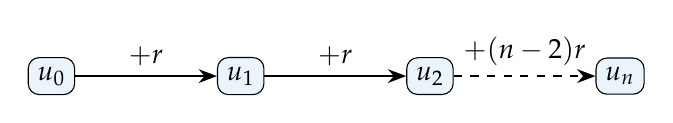
\begin{tikzpicture}[>=Stealth,node distance=18mm]
\node[draw,rounded corners,fill=Sky] (u0) {$u_0$};
\node[draw,rounded corners,fill=Sky,right=of u0] (u1) {$u_1$};
\node[draw,rounded corners,fill=Sky,right=of u1] (u2) {$u_2$};
\node[draw,rounded corners,fill=Sky,right=of u2] (un) {$u_n$};
\draw[->,thick] (u0)--node[above] {$+r$}(u1);
\draw[->,thick] (u1)--node[above] {$+r$}(u2);
\draw[->,thick,dashed] (u2)--node[above] {$+(n-2)r$}(un);
\end{tikzpicture}
\end{center}

Trois nombres $x,y,z$, écrits dans cet ordre, sont trois termes consécutifs d'une suite arithmétique si $y-x=z-y$, c'est-à-dire si $y=\dfrac{x+z}{2}$. Cette dernière quantité est la moyenne arithmétique de $x$ et $z$.

\begin{methode}
Pour modéliser une situation additive : 1) définir $u_n$ et préciser l'unité ; 2) identifier le premier terme ; 3) traduire l'augmentation ou la diminution constante par la raison $r$ ; 4) écrire le terme général ; 5) répondre par une phrase contextualisée.
\end{methode}

\begin{exemple}
Un commerce vend $480$ unités le premier mois puis $25$ unités de plus chaque mois. Avec $u_1=480$ et $r=25$, on obtient $u_n=480+25(n-1)$. Ainsi $u_{12}=755$ : le commerce prévoit $755$ unités vendues au douzième mois.
\end{exemple}

\subsection{Somme de termes arithmétiques}
Pour $n+1$ termes de $u_0$ à $u_n$,
\[
u_0+u_1+\cdots+u_n=(n+1)\frac{u_0+u_n}{2}.
\]
La formule se mémorise sous la forme : \emph{nombre de termes multiplié par la moyenne du premier et du dernier terme}.

\begin{erreur}
Dans $u_3+u_4+\cdots+u_{12}$, il y a $12-3+1=10$ termes, et non $9$ ni $12$.
\end{erreur}

\subsection{Suite géométrique}
\begin{retenir}
Une suite $(u_n)$ est \textbf{géométrique} lorsqu'il existe un réel $q$ tel que $u_{n+1}=q u_n$. Si le premier terme est $u_0$, alors $u_n=u_0q^n$. Si le premier terme est $u_1$, alors $u_n=u_1q^{n-1}$.
\end{retenir}

\begin{center}
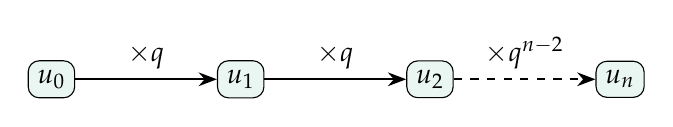
\begin{tikzpicture}[>=Stealth,node distance=18mm]
\node[draw,rounded corners,fill=Mint] (u0) {$u_0$};
\node[draw,rounded corners,fill=Mint,right=of u0] (u1) {$u_1$};
\node[draw,rounded corners,fill=Mint,right=of u1] (u2) {$u_2$};
\node[draw,rounded corners,fill=Mint,right=of u2] (un) {$u_n$};
\draw[->,thick] (u0)--node[above] {$\times q$}(u1);
\draw[->,thick] (u1)--node[above] {$\times q$}(u2);
\draw[->,thick,dashed] (u2)--node[above] {$\times q^{n-2}$}(un);
\end{tikzpicture}
\end{center}

Une hausse de $t\,\%$ correspond à $q=1+\dfrac{t}{100}$ ; une baisse de $t\,\%$ à $q=1-\dfrac{t}{100}$. Trois termes positifs $x,y,z$ sont consécutifs dans une suite géométrique si $y^2=xz$ ; $y=\sqrt{xz}$ est leur moyenne géométrique.

Pour $q\neq1$,
\[
u_0+u_1+\cdots+u_n=u_0\frac{1-q^{n+1}}{1-q}.
\]

\subsection{Algorithmique : calculer une somme}
\begin{lstlisting}[style=python]
def somme_carres(n):
    s = 0
    for k in range(1, n + 1):
        s = s + k**2
    return s
\end{lstlisting}
L'accumulateur \texttt{s} contient la somme partielle ; le compteur \texttt{k} parcourt les entiers de $1$ à $n$.

\sessionheader{1}{15/09/2026}{B : 2 h -- C : 1 h}{Suite arithmétique : reconnaître et modéliser}{Suites numériques}
    \begin{objectifs}\begin{itemize}\item Reconnaître une évolution additive.\item Déterminer la raison.\item Définir une suite dans un contexte.\end{itemize}\end{objectifs}
    \begin{automatismes}\begin{enumerate}\item Écrire le coefficient multiplicateur d'une hausse de $10\,\%$. \rep{$1+\dfrac{10}{100}=1,10$}\item Calculer $u_4$ si $u_0=14$ et $u_{n+1}=u_n+3$. \rep{$u_4=26$}\item Combien de termes de $u_3$ à $u_{15}$ ? \rep{$15-3+1=13$}\item Donner le coefficient d'une baisse de $8\,\%$. \rep{$0{,}92$}\item Donner la raison de $12,12+4,12+2\times4,\ldots$. \rep{$r=4$}\end{enumerate}\end{automatismes}
    \begin{prerequis}Relire la dernière trace écrite et savoir effectuer les calculs élémentaires mobilisés aujourd'hui. Avant l'activité, faire reformuler les mots-clés : reconnaître une évolution additive et déterminer la raison.\end{prerequis}

    \begin{activite}
    Une association compte $320$ adhérents. Elle prévoit d'en gagner $18$ chaque année. On note $u_n$ l'effectif après $n$ années. Calculer $u_0,u_1,u_2$. Quelle opération fait passer d'un terme au suivant ? Écrire une relation entre $u_{n+1}$ et $u_n$, puis prévoir $u_5$.
    \begin{center}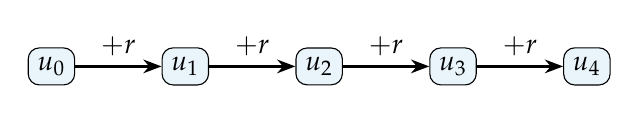
\begin{tikzpicture}[>=Stealth,node distance=17mm]
\foreach \i in {0,...,4}{\node[draw,rounded corners,fill=Sky] (u\i) at (1.7*\i,0) {$u_\i$};}
\foreach \i [evaluate=\i as \j using int(\i+1)] in {0,...,3}{\draw[->,thick] (u\i)--node[above] {$ +r $}(u\j);}
\end{tikzpicture}\end{center}
    \end{activite}
    \enseignant{$u_0=320$, $u_1=338$, $u_2=356$ ; on ajoute $18$. Donc $u_{n+1}=u_n+18$ et $u_5=410$. Faire verbaliser la donnée qui déclenche le choix de méthode.}

    \begin{traceecrite}Une suite est arithmétique lorsque $u_{n+1}-u_n=r$ est constant. Dans une situation, une augmentation absolue constante conduit à une suite arithmétique.\end{traceecrite}

    \begin{exemple}
    Reprendre les données de l'activité et rédiger la solution dans l'ordre : définition des objets, propriété utilisée, calcul exact ou approché, puis phrase de réponse. La réponse modèle figure dans l'édition enseignant.
    \end{exemple}
    \enseignant{$u_0=320$, $u_1=338$, $u_2=356$ ; on ajoute $18$. Donc $u_{n+1}=u_n+18$ et $u_5=410$.}

    \begin{exercice}[-- essentiel]
    \begin{enumerate}\item La suite $(u_n)$ vérifie $u_0=110$ et $u_{n+1}=u_n+3$. Écrire $u_n$ puis calculer $u_{12}$.\item Une quantité vaut $420$ et baisse de $3\,\%$ par période. Écrire $v_n$ et calculer $v_5$.\item Pour chaque suite, préciser si le modèle est arithmétique ou géométrique et justifier par une différence ou un quotient.\end{enumerate}
    \end{exercice}
    \enseignant{$u_n=110+3n$ et $u_{12}=146$, Pour la seconde, $q=0,97$ et $v_n=420\times q^n$ ; le troisième item se justifie par la constance de la différence ou du quotient,}

    \manuelref{Calao, cours p. 18--21 ; exercices p. 24, n° 1 à 3}
\ExoSession{1}

    \begin{dm}Reprendre l'exercice d'entraînement 2 avec les données suivantes : remplacer la donnée initiale par $125$ et le taux ou la raison par $3$. Rédiger en quatre lignes : données, formule, calcul, conclusion.\end{dm}
    \enseignant{La correction dépend de l'exercice repris. Vérifier surtout la cohérence du modèle, le nombre d'itérations, l'arrondi et la phrase de conclusion.}

    \begin{sortie}Sur une demi-feuille : écrire la règle principale de la séance, traiter un exemple très court et indiquer son degré de confiance de 1 à 4. Question(s) essentielle(s) du jour : 1, 2 et 3.\end{sortie}

    \ifprof
    \begin{methode}
    \textbf{Conduite en 1 h :} 7 min d'automatismes ; 10 min de mise en commun et trace ; 28 min d'exercices essentiels ; 5 min de correction ; 3 min de billet de sortie.\\
    \textbf{Conduite en 2 h :} ajouter 20 min de recherche de l'activité, 20 min d'institutionnalisation, un second exercice autonome et 10 min de correction comparée.\\
    \textbf{Différenciation :} fournir aux élèves fragiles une fiche à quatre cases (données, modèle, calcul, conclusion). Demander aux élèves rapides de produire un contre-exemple, une justification ou une seconde méthode.
    \end{methode}
    \fi
\sessionheader{2}{17/09/2026}{B : 1 h -- C : 2 h}{Suite arithmétique : terme général}{Suites numériques}
\begin{objectifs}\begin{itemize}\item Passer de la récurrence au terme général.\item Calculer un terme éloigné.\item Interpréter le rang.\end{itemize}\end{objectifs}
\begin{automatismes}\begin{enumerate}\item Réduire $3x+5-x+2$. \rep{$2x+7$}\item Combien de termes de $u_3$ à $u_{15}$ ? \rep{$15-3+1=13$}\item Donner le coefficient d'une baisse de $8\,\%$. \rep{$0{,}92$}\item Donner la raison de $12,12+5,12+2\times5,\ldots$. \rep{$r=5$}\item Calculer $u_4$ si $u_0=15$ et $u_{n+1}=u_n+3$. \rep{$u_4=27$}\end{enumerate}\end{automatismes}
\begin{prerequis}Relire la dernière trace écrite et savoir effectuer les calculs élémentaires mobilisés aujourd'hui. Avant l'activité, faire reformuler les mots-clés : passer de la récurrence au terme général et calculer un terme éloigné.\end{prerequis}

\begin{activite}
Un magasin possède $1\,250$ cartes de fidélité actives au rang $0$ et en gagne $75$ par mois. Sans calculer tous les termes, déterminer l'effectif au rang $n$, puis au rang $18$. Expliquer le rôle de $18$ dans le calcul.

\end{activite}
\enseignant{$u_n=1\,250+75n$, donc $u_{18}=2\,600$. Le nombre $18$ compte les augmentations depuis le rang $0$. Faire verbaliser la donnée qui déclenche le choix de méthode.}

\begin{traceecrite}Si $(u_n)$ est arithmétique de raison $r$, alors $u_n=u_0+nr$ ou $u_n=u_1+(n-1)r$, selon le rang du premier terme.\end{traceecrite}

\begin{exemple}
Reprendre les données de l'activité et rédiger la solution dans l'ordre : définition des objets, propriété utilisée, calcul exact ou approché, puis phrase de réponse. La réponse modèle figure dans l'édition enseignant.
\end{exemple}
\enseignant{$u_n=1\,250+75n$, donc $u_{18}=2\,600$. Le nombre $18$ compte les augmentations depuis le rang $0$.}

\begin{exercice}[-- essentiel]
\begin{enumerate}\item La suite $(u_n)$ vérifie $u_0=120$ et $u_{n+1}=u_n+4$. Écrire $u_n$ puis calculer $u_{12}$.\item Une quantité vaut $440$ et baisse de $4\,\%$ par période. Écrire $v_n$ et calculer $v_5$.\item Pour chaque suite, préciser si le modèle est arithmétique ou géométrique et justifier par une différence ou un quotient.\end{enumerate}
\end{exercice}
\enseignant{$u_n=120+4n$ et $u_{12}=168$, Pour la seconde, $q=0,96$ et $v_n=440\times q^n$ ; le troisième item se justifie par la constance de la différence ou du quotient,}

\manuelref{Calao, cours p. 18--21 ; exercices p. 24, n° 5 à 8}
\ExoSession{2}

\begin{dm}Reprendre l'exercice d'entraînement 3 avec les données suivantes : remplacer la donnée initiale par $130$ et le taux ou la raison par $4$. Rédiger en quatre lignes : données, formule, calcul, conclusion.\end{dm}
\enseignant{La correction dépend de l'exercice repris. Vérifier surtout la cohérence du modèle, le nombre d'itérations, l'arrondi et la phrase de conclusion.}

\begin{sortie}Sur une demi-feuille : écrire la règle principale de la séance, traiter un exemple très court et indiquer son degré de confiance de 1 à 4. Question(s) essentielle(s) du jour : 1 et 2.\end{sortie}

\ifprof
\begin{methode}
\textbf{Conduite en 1 h :} 7 min d'automatismes ; 10 min de mise en commun et trace ; 28 min d'exercices essentiels ; 5 min de correction ; 3 min de billet de sortie.\\
\textbf{Conduite en 2 h :} ajouter 20 min de recherche de l'activité, 20 min d'institutionnalisation, un second exercice autonome et 10 min de correction comparée.\\
\textbf{Différenciation :} fournir aux élèves fragiles une fiche à quatre cases (données, modèle, calcul, conclusion). Demander aux élèves rapides de produire un contre-exemple, une justification ou une seconde méthode.
\end{methode}
\fi
\sessionheader{3}{22/09/2026}{B : 2 h -- C : 1 h}{Somme des termes d'une suite arithmétique}{Suites numériques}
\begin{objectifs}\begin{itemize}\item Compter les termes d'une somme.\item Appliquer la formule.\item Contrôler l'ordre de grandeur.\end{itemize}\end{objectifs}
\begin{automatismes}\begin{enumerate}\item Calculer $20\,\%$ de $120$. \rep{$24$}\item Donner le coefficient d'une baisse de $8\,\%$. \rep{$0{,}92$}\item Donner la raison de $12,12+6,12+2\times6,\ldots$. \rep{$r=6$}\item Calculer $u_4$ si $u_0=16$ et $u_{n+1}=u_n+3$. \rep{$u_4=28$}\item Combien de termes de $u_3$ à $u_{15}$ ? \rep{$15-3+1=13$}\end{enumerate}\end{automatismes}
\begin{prerequis}Relire la dernière trace écrite et savoir effectuer les calculs élémentaires mobilisés aujourd'hui. Avant l'activité, faire reformuler les mots-clés : compter les termes d'une somme et appliquer la formule.\end{prerequis}

\begin{activite}
Une entreprise verse une prime mensuelle : $45$ euros le premier mois, puis $5$ euros de plus chaque mois. Calculer le total versé pendant les douze premiers mois de trois façons : somme explicite, regroupement premier-dernier, formule.

\end{activite}
\enseignant{$u_{12}=45+11\times5=100$. Le total vaut $12\times\dfrac{45+100}{2}=870$ euros. Faire verbaliser la donnée qui déclenche le choix de méthode.}

\begin{traceecrite}Une somme de termes arithmétiques vaut $\text{nombre de termes}\times\dfrac{\text{premier}+\text{dernier}}2$. De $u_p$ à $u_q$, il y a $q-p+1$ termes.\end{traceecrite}

\begin{exemple}
Reprendre les données de l'activité et rédiger la solution dans l'ordre : définition des objets, propriété utilisée, calcul exact ou approché, puis phrase de réponse. La réponse modèle figure dans l'édition enseignant.
\end{exemple}
\enseignant{$u_{12}=45+11\times5=100$. Le total vaut $12\times\dfrac{45+100}{2}=870$ euros.}

\begin{exercice}[-- essentiel]
\begin{enumerate}\item La suite $(u_n)$ vérifie $u_0=130$ et $u_{n+1}=u_n+5$. Écrire $u_n$ puis calculer $u_{12}$.\item Une quantité vaut $460$ et baisse de $5\,\%$ par période. Écrire $v_n$ et calculer $v_5$.\item Pour chaque suite, préciser si le modèle est arithmétique ou géométrique et justifier par une différence ou un quotient.\end{enumerate}
\end{exercice}
\enseignant{$u_n=130+5n$ et $u_{12}=190$, Pour la seconde, $q=0,95$ et $v_n=460\times q^n$ ; le troisième item se justifie par la constance de la différence ou du quotient,}

\manuelref{Calao, cours p. 20--21 ; exercices p. 24, n° 11 à 13, puis p. 28, n° 43--44}
\ExoSession{3}

\begin{dm}Reprendre l'exercice d'entraînement 2 avec les données suivantes : remplacer la donnée initiale par $135$ et le taux ou la raison par $5$. Rédiger en quatre lignes : données, formule, calcul, conclusion.\end{dm}
\enseignant{La correction dépend de l'exercice repris. Vérifier surtout la cohérence du modèle, le nombre d'itérations, l'arrondi et la phrase de conclusion.}

\begin{sortie}Sur une demi-feuille : écrire la règle principale de la séance, traiter un exemple très court et indiquer son degré de confiance de 1 à 4. Question(s) essentielle(s) du jour : 1, 2 et 3.\end{sortie}

\ifprof
\begin{methode}
\textbf{Conduite en 1 h :} 7 min d'automatismes ; 10 min de mise en commun et trace ; 28 min d'exercices essentiels ; 5 min de correction ; 3 min de billet de sortie.\\
\textbf{Conduite en 2 h :} ajouter 20 min de recherche de l'activité, 20 min d'institutionnalisation, un second exercice autonome et 10 min de correction comparée.\\
\textbf{Différenciation :} fournir aux élèves fragiles une fiche à quatre cases (données, modèle, calcul, conclusion). Demander aux élèves rapides de produire un contre-exemple, une justification ou une seconde méthode.
\end{methode}
\fi
\sessionheader{4}{24/09/2026}{B : 1 h -- C : 2 h}{Suite géométrique : reconnaître et modéliser}{Suites numériques}
    \begin{objectifs}\begin{itemize}\item Reconnaître une évolution multiplicative.\item Passer d'un taux à un coefficient.\item Comparer arithmétique et géométrique.\end{itemize}\end{objectifs}
    \begin{automatismes}\begin{enumerate}\item Écrire le coefficient multiplicateur d'une hausse de $25\,\%$. \rep{$1+\dfrac{25}{100}=1,25$}\item Donner la raison de $12,12+7,12+2\times7,\ldots$. \rep{$r=7$}\item Calculer $u_4$ si $u_0=17$ et $u_{n+1}=u_n+3$. \rep{$u_4=29$}\item Combien de termes de $u_3$ à $u_{15}$ ? \rep{$15-3+1=13$}\item Donner le coefficient d'une baisse de $8\,\%$. \rep{$0{,}92$}\end{enumerate}\end{automatismes}
    \begin{prerequis}Relire la dernière trace écrite et savoir effectuer les calculs élémentaires mobilisés aujourd'hui. Avant l'activité, faire reformuler les mots-clés : reconnaître une évolution multiplicative et passer d'un taux à un coefficient.\end{prerequis}

    \begin{activite}
    Une boutique en ligne augmente son nombre de visiteurs de $6\,\%$ par mois à partir de $8\,000$ visiteurs. Calculer les trois premières valeurs. Comparer les différences puis les quotients. Identifier la nature de la suite.
    \begin{center}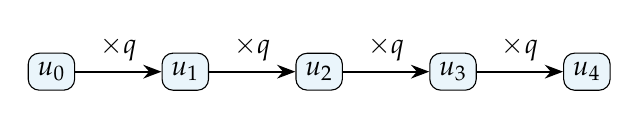
\begin{tikzpicture}[>=Stealth,node distance=17mm]
\foreach \i in {0,...,4}{\node[draw,rounded corners,fill=Sky] (u\i) at (1.7*\i,0) {$u_\i$};}
\foreach \i [evaluate=\i as \j using int(\i+1)] in {0,...,3}{\draw[->,thick] (u\i)--node[above] {$ \times q $}(u\j);}
\end{tikzpicture}\end{center}
    \end{activite}
    \enseignant{Le coefficient est $1{,}06$ : $8\,000$, $8\,480$, $8\,988{,}8$. Les quotients valent $1{,}06$ ; la suite est géométrique. Faire verbaliser la donnée qui déclenche le choix de méthode.}

    \begin{traceecrite}Une suite est géométrique lorsque $\dfrac{u_{n+1}}{u_n}=q$ est constant (termes non nuls). Une évolution relative constante conduit à une suite géométrique.\end{traceecrite}

    \begin{exemple}
    Reprendre les données de l'activité et rédiger la solution dans l'ordre : définition des objets, propriété utilisée, calcul exact ou approché, puis phrase de réponse. La réponse modèle figure dans l'édition enseignant.
    \end{exemple}
    \enseignant{Le coefficient est $1{,}06$ : $8\,000$, $8\,480$, $8\,988{,}8$. Les quotients valent $1{,}06$ ; la suite est géométrique.}

    \begin{exercice}[-- essentiel]
    \begin{enumerate}\item La suite $(u_n)$ vérifie $u_0=140$ et $u_{n+1}=u_n+6$. Écrire $u_n$ puis calculer $u_{12}$.\item Une quantité vaut $480$ et baisse de $6\,\%$ par période. Écrire $v_n$ et calculer $v_5$.\item Pour chaque suite, préciser si le modèle est arithmétique ou géométrique et justifier par une différence ou un quotient.\end{enumerate}
    \end{exercice}
    \enseignant{$u_n=140+6n$ et $u_{12}=212$, Pour la seconde, $q=0,94$ et $v_n=480\times q^n$ ; le troisième item se justifie par la constance de la différence ou du quotient,}

    \manuelref{Calao, cours p. 23--25 ; exercices p. 25, n° 14 à 18}
\ExoSession{4}

    \begin{dm}Reprendre l'exercice d'entraînement 3 avec les données suivantes : remplacer la donnée initiale par $140$ et le taux ou la raison par $6$. Rédiger en quatre lignes : données, formule, calcul, conclusion.\end{dm}
    \enseignant{La correction dépend de l'exercice repris. Vérifier surtout la cohérence du modèle, le nombre d'itérations, l'arrondi et la phrase de conclusion.}

    \begin{sortie}Sur une demi-feuille : écrire la règle principale de la séance, traiter un exemple très court et indiquer son degré de confiance de 1 à 4. Question(s) essentielle(s) du jour : 1 et 2.\end{sortie}

    \ifprof
    \begin{methode}
    \textbf{Conduite en 1 h :} 7 min d'automatismes ; 10 min de mise en commun et trace ; 28 min d'exercices essentiels ; 5 min de correction ; 3 min de billet de sortie.\\
    \textbf{Conduite en 2 h :} ajouter 20 min de recherche de l'activité, 20 min d'institutionnalisation, un second exercice autonome et 10 min de correction comparée.\\
    \textbf{Différenciation :} fournir aux élèves fragiles une fiche à quatre cases (données, modèle, calcul, conclusion). Demander aux élèves rapides de produire un contre-exemple, une justification ou une seconde méthode.
    \end{methode}
    \fi
\sessionheader{5}{29/09/2026}{B : 2 h -- C : 1 h}{Suite géométrique : terme général et somme}{Suites numériques}
\begin{objectifs}\begin{itemize}\item Écrire le terme général.\item Calculer une somme géométrique.\item Interpréter une évolution cumulée.\end{itemize}\end{objectifs}
\begin{automatismes}\begin{enumerate}\item Réduire $3x+8-x+2$. \rep{$2x+10$}\item Calculer $u_4$ si $u_0=18$ et $u_{n+1}=u_n+3$. \rep{$u_4=30$}\item Combien de termes de $u_3$ à $u_{15}$ ? \rep{$15-3+1=13$}\item Donner le coefficient d'une baisse de $8\,\%$. \rep{$0{,}92$}\item Donner la raison de $12,12+8,12+2\times8,\ldots$. \rep{$r=8$}\end{enumerate}\end{automatismes}
\begin{prerequis}Relire la dernière trace écrite et savoir effectuer les calculs élémentaires mobilisés aujourd'hui. Avant l'activité, faire reformuler les mots-clés : écrire le terme général et calculer une somme géométrique.\end{prerequis}

\begin{activite}
Un capital de $250\,000$ Ar est placé à $4\,\%$ par an, intérêts composés. Écrire le capital $C_n$ après $n$ années. Calculer $C_6$, puis la somme $C_0+\cdots+C_6$ et expliquer ce que cette dernière somme représente mathématiquement et pourquoi elle n'est pas le capital final.

\end{activite}
\enseignant{$C_n=250\,000\times1{,}04^n$ et $C_6\approx316\,330$ Ar. La somme est la somme de sept états successifs, pas une accumulation réelle du placement. Faire verbaliser la donnée qui déclenche le choix de méthode.}

\begin{traceecrite}Si $(u_n)$ est géométrique de raison $q$, $u_n=u_0q^n$ ou $u_n=u_1q^{n-1}$. Pour $q\neq1$, $u_0+\cdots+u_n=u_0\dfrac{1-q^{n+1}}{1-q}$.\end{traceecrite}

\begin{exemple}
Reprendre les données de l'activité et rédiger la solution dans l'ordre : définition des objets, propriété utilisée, calcul exact ou approché, puis phrase de réponse. La réponse modèle figure dans l'édition enseignant.
\end{exemple}
\enseignant{$C_n=250\,000\times1{,}04^n$ et $C_6\approx316\,330$ Ar. La somme est la somme de sept états successifs, pas une accumulation réelle du placement.}

\begin{exercice}[-- essentiel]
\begin{enumerate}\item La suite $(u_n)$ vérifie $u_0=150$ et $u_{n+1}=u_n+2$. Écrire $u_n$ puis calculer $u_{12}$.\item Une quantité vaut $500$ et baisse de $2\,\%$ par période. Écrire $v_n$ et calculer $v_5$.\item Pour chaque suite, préciser si le modèle est arithmétique ou géométrique et justifier par une différence ou un quotient.\end{enumerate}
\end{exercice}
\enseignant{$u_n=150+2n$ et $u_{12}=174$, Pour la seconde, $q=0,98$ et $v_n=500\times q^n$ ; le troisième item se justifie par la constance de la différence ou du quotient,}

\manuelref{Calao, cours p. 25--28 ; exercices p. 25, n° 19 à 25, puis p. 28, n° 42--44}
\ExoSession{5}

\begin{dm}Reprendre l'exercice d'entraînement 2 avec les données suivantes : remplacer la donnée initiale par $145$ et le taux ou la raison par $7$. Rédiger en quatre lignes : données, formule, calcul, conclusion.\end{dm}
\enseignant{La correction dépend de l'exercice repris. Vérifier surtout la cohérence du modèle, le nombre d'itérations, l'arrondi et la phrase de conclusion.}

\begin{sortie}Sur une demi-feuille : écrire la règle principale de la séance, traiter un exemple très court et indiquer son degré de confiance de 1 à 4. Question(s) essentielle(s) du jour : 1, 2 et 3.\end{sortie}

\ifprof
\begin{methode}
\textbf{Conduite en 1 h :} 7 min d'automatismes ; 10 min de mise en commun et trace ; 28 min d'exercices essentiels ; 5 min de correction ; 3 min de billet de sortie.\\
\textbf{Conduite en 2 h :} ajouter 20 min de recherche de l'activité, 20 min d'institutionnalisation, un second exercice autonome et 10 min de correction comparée.\\
\textbf{Différenciation :} fournir aux élèves fragiles une fiche à quatre cases (données, modèle, calcul, conclusion). Demander aux élèves rapides de produire un contre-exemple, une justification ou une seconde méthode.
\end{methode}
\fi
\sessionheader{6}{01/10/2026}{B : 1 h -- C : 2 h}{Bilan et évaluation formative}{Suites numériques}
\begin{objectifs}\begin{itemize}\item Choisir le bon modèle.\item Mobiliser les formules.\item Analyser ses erreurs.\end{itemize}\end{objectifs}
\begin{automatismes}\begin{enumerate}\item Calculer $5\,\%$ de $180$. \rep{$9$}\item Combien de termes de $u_3$ à $u_{15}$ ? \rep{$15-3+1=13$}\item Donner le coefficient d'une baisse de $8\,\%$. \rep{$0{,}92$}\item Donner la raison de $12,12+9,12+2\times9,\ldots$. \rep{$r=9$}\item Calculer $u_4$ si $u_0=19$ et $u_{n+1}=u_n+3$. \rep{$u_4=31$}\end{enumerate}\end{automatismes}
\begin{prerequis}Relire la dernière trace écrite et savoir effectuer les calculs élémentaires mobilisés aujourd'hui. Avant l'activité, faire reformuler les mots-clés : choisir le bon modèle et mobiliser les formules.\end{prerequis}

\begin{activite}
Classer huit situations selon trois catégories : arithmétique, géométrique, ni l'une ni l'autre. Pour chaque situation, souligner le mot ou la donnée qui justifie le choix, puis choisir la formule adaptée.

\end{activite}
\enseignant{Une variation absolue constante indique le modèle arithmétique ; un pourcentage ou coefficient constant indique le modèle géométrique ; sinon aucun des deux n'est garanti. Faire verbaliser la donnée qui déclenche le choix de méthode.}

\begin{traceecrite}Avant de calculer, identifier : type de suite, premier rang, raison, terme ou somme demandé. La conclusion précise l'unité et le rang.\end{traceecrite}

\begin{exemple}
Reprendre les données de l'activité et rédiger la solution dans l'ordre : définition des objets, propriété utilisée, calcul exact ou approché, puis phrase de réponse. La réponse modèle figure dans l'édition enseignant.
\end{exemple}
\enseignant{Une variation absolue constante indique le modèle arithmétique ; un pourcentage ou coefficient constant indique le modèle géométrique ; sinon aucun des deux n'est garanti.}

\begin{exercice}[-- essentiel]
\begin{enumerate}\item La suite $(u_n)$ vérifie $u_0=160$ et $u_{n+1}=u_n+3$. Écrire $u_n$ puis calculer $u_{12}$.\item Une quantité vaut $520$ et baisse de $3\,\%$ par période. Écrire $v_n$ et calculer $v_5$.\item Pour chaque suite, préciser si le modèle est arithmétique ou géométrique et justifier par une différence ou un quotient.\end{enumerate}
\end{exercice}
\enseignant{$u_n=160+3n$ et $u_{12}=196$, Pour la seconde, $q=0,97$ et $v_n=520\times q^n$ ; le troisième item se justifie par la constance de la différence ou du quotient,}

\manuelref{Calao, p. 29, n° 49 à 52}
\ExoSession{6}

\begin{dm}Reprendre l'exercice d'entraînement 3 avec les données suivantes : remplacer la donnée initiale par $150$ et le taux ou la raison par $2$. Rédiger en quatre lignes : données, formule, calcul, conclusion.\end{dm}
\enseignant{La correction dépend de l'exercice repris. Vérifier surtout la cohérence du modèle, le nombre d'itérations, l'arrondi et la phrase de conclusion.}

\begin{sortie}Sur une demi-feuille : écrire la règle principale de la séance, traiter un exemple très court et indiquer son degré de confiance de 1 à 4. Question(s) essentielle(s) du jour : 1 et 2.\end{sortie}

\ifprof
\begin{methode}
\textbf{Conduite en 1 h :} 7 min d'automatismes ; 10 min de mise en commun et trace ; 28 min d'exercices essentiels ; 5 min de correction ; 3 min de billet de sortie.\\
\textbf{Conduite en 2 h :} ajouter 20 min de recherche de l'activité, 20 min d'institutionnalisation, un second exercice autonome et 10 min de correction comparée.\\
\textbf{Différenciation :} fournir aux élèves fragiles une fiche à quatre cases (données, modèle, calcul, conclusion). Demander aux élèves rapides de produire un contre-exemple, une justification ou une seconde méthode.
\end{methode}
\fi


\chapter{Fonctions exponentielles}
\competences{modéliser une évolution continue, changer de registre, calculer, interpréter}
\section{Cours de référence}
Pour $a>0$, la fonction $x\mapsto a^x$ prolonge à tous les réels les puissances entières de $a$. Elle vérifie $a^0=1$ et $a^{-x}=\dfrac{1}{a^x}$.

\begin{center}
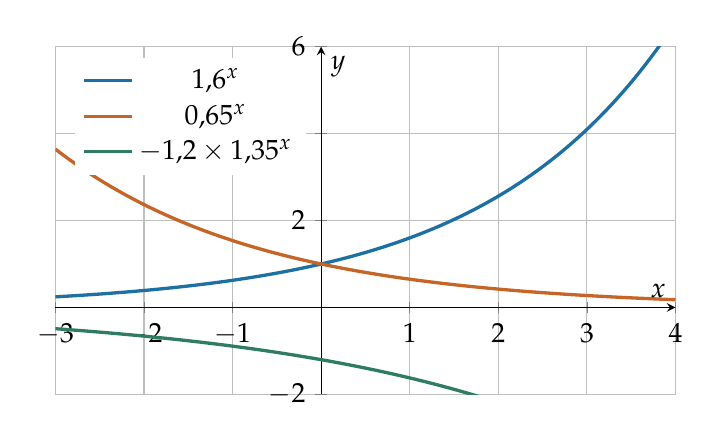
\begin{tikzpicture}
\begin{axis}[width=.78\textwidth,height=6cm,axis lines=middle,xmin=-3,xmax=4,ymin=-2,ymax=6,grid=major,xlabel={$x$},ylabel={$y$},legend style={at={(.03,.97)},anchor=north west,draw=none,fill=white}]
\addplot[Blue,very thick,samples=100,domain=-3:4]{1.6^x};\addlegendentry{$1{,}6^x$}
\addplot[Orange,very thick,samples=100,domain=-3:4]{0.65^x};\addlegendentry{$0{,}65^x$}
\addplot[Green,very thick,samples=100,domain=-3:4]{-1.2*1.35^x};\addlegendentry{$-1{,}2\times1{,}35^x$}
\end{axis}
\end{tikzpicture}
\end{center}

\begin{retenir}
Si $a>1$, $x\mapsto a^x$ est strictement croissante. Si $0<a<1$, elle est strictement décroissante. Pour $f(x)=ka^x$, multiplier par $k<0$ inverse le sens de variation. Dans tous les cas, $a^x>0$.
\end{retenir}

Pour $a>0$ et tous réels $x,y$ :
\[
a^{x+y}=a^xa^y,\qquad a^{x-y}=\frac{a^x}{a^y},\qquad (a^x)^y=a^{xy}.
\]

\begin{erreur}
En général, $a^x+a^y\neq a^{x+y}$. Les propriétés portent sur les produits et les quotients, pas sur les sommes.
\end{erreur}

\subsection{Évolutions et taux moyen}
Une quantité de valeur initiale $V_0$ soumise à une évolution relative constante de coefficient $q$ se modélise par $V(t)=V_0q^t$. Si un coefficient global $Q$ résulte de $n$ évolutions identiques, le coefficient moyen est $q=Q^{\frac1n}$ et le taux moyen est $t=q-1$.

\begin{exemple}
Un chiffre d'affaires passe de $80\,000$ à $95\,000$ euros en quatre ans. Le coefficient global vaut $Q=\dfrac{95\,000}{80\,000}=1{,}1875$. Le coefficient annuel moyen est $q=1{,}1875^{\frac14}\approx1{,}0440$ : le taux annuel moyen est donc environ $4{,}40\,\%$.
\end{exemple}

\subsection{Résoudre et interpréter}
Lorsque les deux membres peuvent être écrits avec la même base, on utilise l'injectivité : pour $a>0$ et $a\neq1$, $a^u=a^v$ équivaut à $u=v$. Sinon, une résolution graphique ou numérique donne une valeur approchée ; le logarithme décimal, étudié ensuite, donnera une formule.

\sessionheader{7}{06/10/2026}{B : 2 h -- C : 1 h}{Définition et sens de variation de $a^x$}{Fonctions exponentielles}
\begin{objectifs}\begin{itemize}\item Donner du sens à $a^x$.\item Relier base et variation.\item Lire des courbes.\end{itemize}\end{objectifs}
\begin{automatismes}\begin{enumerate}\item Écrire le coefficient multiplicateur d'une hausse de $10\,\%$. \rep{$1+\dfrac{10}{100}=1,10$}\item Comparer $1{,}04^3$ et $1{,}04^7$. \rep{$1{,}04^3<1{,}04^7$}\item Calculer $2^4\times2^3$. \rep{$2^7$}\item Écrire $5^{-2}$ sous forme de fraction. \rep{$\dfrac1{25}$}\item La fonction $x\mapsto0{,}7^x$ est-elle croissante ? \rep{Non, elle est décroissante.}\end{enumerate}\end{automatismes}
\begin{prerequis}Relire la dernière trace écrite et savoir effectuer les calculs élémentaires mobilisés aujourd'hui. Avant l'activité, faire reformuler les mots-clés : donner du sens à $a^x$ et relier base et variation.\end{prerequis}

\begin{activite}
À l'aide d'une calculatrice, compléter un tableau de valeurs de $1{,}5^x$ et $0{,}7^x$ pour $x=-2,-1,0,1,2,3$. Tracer les points, conjecturer les variations et identifier le point commun aux deux courbes.
\begin{center}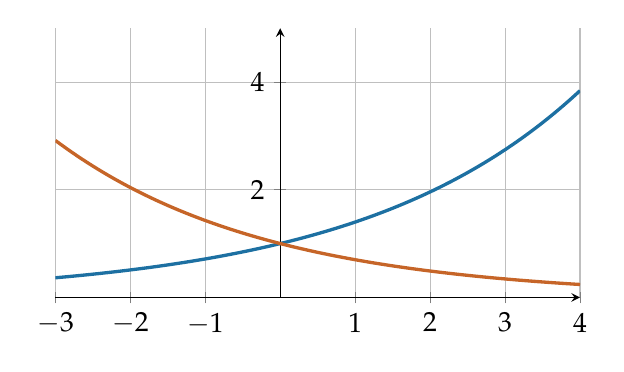
\begin{tikzpicture}\begin{axis}[width=.68\textwidth,height=5cm,axis lines=middle,xmin=-3,xmax=4,ymin=0,ymax=5,grid=major]\addplot[Blue,very thick,samples=100,domain=-3:4]{1.4^x};\addplot[Orange,very thick,samples=100,domain=-3:4]{.7^x};\end{axis}\end{tikzpicture}\end{center}
\end{activite}
\enseignant{$a^0=1$, donc les courbes passent par $(0,1)$. La première croît et la seconde décroît. Faire verbaliser la donnée qui déclenche le choix de méthode.}

\begin{traceecrite}Pour $a>0$, $a^x$ est défini pour tout réel $x$. La fonction est croissante si $a>1$ et décroissante si $0<a<1$.\end{traceecrite}

\begin{exemple}
Reprendre les données de l'activité et rédiger la solution dans l'ordre : définition des objets, propriété utilisée, calcul exact ou approché, puis phrase de réponse. La réponse modèle figure dans l'édition enseignant.
\end{exemple}
\enseignant{$a^0=1$, donc les courbes passent par $(0,1)$. La première croît et la seconde décroît.}

\begin{exercice}[-- essentiel]
\begin{enumerate}\item Simplifier $3^{x+4}\div3^x$ et $(2^x)^3$.\item Étudier le sens de variation de $f(x)=4\times1{,}04^x$ et $g(x)=-4\times0{,}8^x$.\item Une valeur initiale de $1350$ augmente de $4\,\%$ par an. Donner le modèle et calculer la valeur après $6$ ans.\end{enumerate}
\end{exercice}
\enseignant{$3^4$ et $2^{3x}$. $f$ est croissante ; $0{,}8^x$ est décroissante et le coefficient négatif rend $g$ croissante. Le modèle est $V(t)=1350\times\left(1+\dfrac{4}{100}\right)^t$.}

\manuelref{Calao, cours p. 42--47 ; exercices p. 48, n° 1 à 8}
\ExoSession{7}

\begin{dm}Reprendre l'exercice d'entraînement 2 avec les données suivantes : remplacer la donnée initiale par $155$ et le taux ou la raison par $3$. Rédiger en quatre lignes : données, formule, calcul, conclusion.\end{dm}
\enseignant{La correction dépend de l'exercice repris. Vérifier surtout la cohérence du modèle, le nombre d'itérations, l'arrondi et la phrase de conclusion.}

\begin{sortie}Sur une demi-feuille : écrire la règle principale de la séance, traiter un exemple très court et indiquer son degré de confiance de 1 à 4. Question(s) essentielle(s) du jour : 1, 2 et 3.\end{sortie}

\ifprof
\begin{methode}
\textbf{Conduite en 1 h :} 7 min d'automatismes ; 10 min de mise en commun et trace ; 28 min d'exercices essentiels ; 5 min de correction ; 3 min de billet de sortie.\\
\textbf{Conduite en 2 h :} ajouter 20 min de recherche de l'activité, 20 min d'institutionnalisation, un second exercice autonome et 10 min de correction comparée.\\
\textbf{Différenciation :} fournir aux élèves fragiles une fiche à quatre cases (données, modèle, calcul, conclusion). Demander aux élèves rapides de produire un contre-exemple, une justification ou une seconde méthode.
\end{methode}
\fi
\sessionheader{8}{08/10/2026}{B : 1 h -- C : 2 h}{Puissances et propriétés algébriques}{Fonctions exponentielles}
\begin{objectifs}\begin{itemize}\item Transformer des puissances.\item Utiliser les exposants négatifs.\item Repérer une règle inapplicable.\end{itemize}\end{objectifs}
\begin{automatismes}\begin{enumerate}\item Réduire $3x+4-x+2$. \rep{$2x+6$}\item Calculer $2^1\times2^3$. \rep{$2^4$}\item Écrire $5^{-2}$ sous forme de fraction. \rep{$\dfrac1{25}$}\item La fonction $x\mapsto0{,}7^x$ est-elle croissante ? \rep{Non, elle est décroissante.}\item Comparer $1{,}04^3$ et $1{,}04^7$. \rep{$1{,}04^3<1{,}04^7$}\end{enumerate}\end{automatismes}
\begin{prerequis}Relire la dernière trace écrite et savoir effectuer les calculs élémentaires mobilisés aujourd'hui. Avant l'activité, faire reformuler les mots-clés : transformer des puissances et utiliser les exposants négatifs.\end{prerequis}

\begin{activite}
Simplifier $2^3\times2^{-5}$, $5^{x+2}\div5^x$ et $(3^x)^2$. Inventer ensuite un contre-exemple numérique à $a^x+a^y=a^{x+y}$.

\end{activite}
\enseignant{On obtient $2^{-2}=\dfrac14$, $5^2=25$ et $3^{2x}$. Avec $a=2,x=y=1$, $2+2\neq4$ ? Ici égalité accidentelle ; choisir $a=3$ : $3+3\neq9$. Faire verbaliser la donnée qui déclenche le choix de méthode.}

\begin{traceecrite}$a^{x+y}=a^xa^y$, $a^{x-y}=\dfrac{a^x}{a^y}$ et $(a^x)^y=a^{xy}$. Ces règles exigent une même base positive.\end{traceecrite}

\begin{exemple}
Reprendre les données de l'activité et rédiger la solution dans l'ordre : définition des objets, propriété utilisée, calcul exact ou approché, puis phrase de réponse. La réponse modèle figure dans l'édition enseignant.
\end{exemple}
\enseignant{On obtient $2^{-2}=\dfrac14$, $5^2=25$ et $3^{2x}$. Avec $a=2,x=y=1$, $2+2\neq4$ ? Ici égalité accidentelle ; choisir $a=3$ : $3+3\neq9$.}

\begin{exercice}[-- essentiel]
\begin{enumerate}\item Simplifier $3^{x+5}\div3^x$ et $(2^x)^3$.\item Étudier le sens de variation de $f(x)=5\times1{,}05^x$ et $g(x)=-5\times0{,}8^x$.\item Une valeur initiale de $1400$ augmente de $5\,\%$ par an. Donner le modèle et calculer la valeur après $6$ ans.\end{enumerate}
\end{exercice}
\enseignant{$3^5$ et $2^{3x}$. $f$ est croissante ; $0{,}8^x$ est décroissante et le coefficient négatif rend $g$ croissante. Le modèle est $V(t)=1400\times\left(1+\dfrac{5}{100}\right)^t$.}

\manuelref{Calao, cours p. 43--45 ; exercices p. 49, n° 9 à 13}
\ExoSession{8}

\begin{dm}Reprendre l'exercice d'entraînement 3 avec les données suivantes : remplacer la donnée initiale par $160$ et le taux ou la raison par $4$. Rédiger en quatre lignes : données, formule, calcul, conclusion.\end{dm}
\enseignant{La correction dépend de l'exercice repris. Vérifier surtout la cohérence du modèle, le nombre d'itérations, l'arrondi et la phrase de conclusion.}

\begin{sortie}Sur une demi-feuille : écrire la règle principale de la séance, traiter un exemple très court et indiquer son degré de confiance de 1 à 4. Question(s) essentielle(s) du jour : 1 et 2.\end{sortie}

\ifprof
\begin{methode}
\textbf{Conduite en 1 h :} 7 min d'automatismes ; 10 min de mise en commun et trace ; 28 min d'exercices essentiels ; 5 min de correction ; 3 min de billet de sortie.\\
\textbf{Conduite en 2 h :} ajouter 20 min de recherche de l'activité, 20 min d'institutionnalisation, un second exercice autonome et 10 min de correction comparée.\\
\textbf{Différenciation :} fournir aux élèves fragiles une fiche à quatre cases (données, modèle, calcul, conclusion). Demander aux élèves rapides de produire un contre-exemple, une justification ou une seconde méthode.
\end{methode}
\fi
\sessionheader{9}{13/10/2026}{B : 2 h -- C : 1 h}{Fonctions $x\mapsto k a^x$ : variations et graphique}{Fonctions exponentielles}
\begin{objectifs}\begin{itemize}\item Étudier $ka^x$.\item Combiner signe et variation.\item Relier formule et graphique.\end{itemize}\end{objectifs}
\begin{automatismes}\begin{enumerate}\item Calculer $20\,\%$ de $100$. \rep{$20$}\item Écrire $5^{-2}$ sous forme de fraction. \rep{$\dfrac1{25}$}\item La fonction $x\mapsto0{,}7^x$ est-elle croissante ? \rep{Non, elle est décroissante.}\item Comparer $1{,}04^3$ et $1{,}04^7$. \rep{$1{,}04^3<1{,}04^7$}\item Calculer $2^2\times2^3$. \rep{$2^5$}\end{enumerate}\end{automatismes}
\begin{prerequis}Relire la dernière trace écrite et savoir effectuer les calculs élémentaires mobilisés aujourd'hui. Avant l'activité, faire reformuler les mots-clés : étudier $ka^x$ et combiner signe et variation.\end{prerequis}

\begin{activite}
Associer les quatre fonctions $2^x$, $0{,}6^x$, $-2^x$ et $-0{,}6^x$ à quatre courbes. Justifier chaque choix par le signe, le point d'ordonnée à l'origine et le sens de variation.
\begin{center}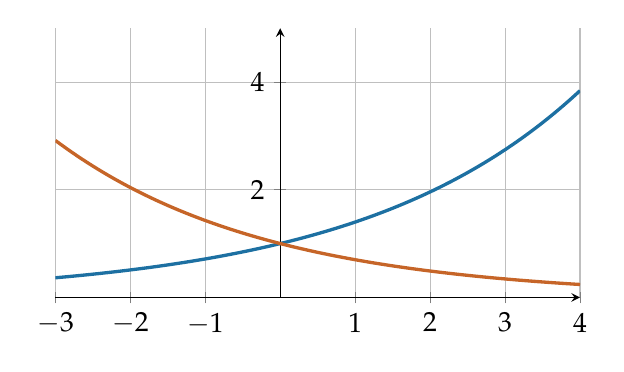
\begin{tikzpicture}\begin{axis}[width=.68\textwidth,height=5cm,axis lines=middle,xmin=-3,xmax=4,ymin=0,ymax=5,grid=major]\addplot[Blue,very thick,samples=100,domain=-3:4]{1.4^x};\addplot[Orange,very thick,samples=100,domain=-3:4]{.7^x};\end{axis}\end{tikzpicture}\end{center}
\end{activite}
\enseignant{Toutes ont une valeur absolue égale à $1$ en $0$. Le signe distingue les deux paires ; la base et le signe du coefficient déterminent la variation. Faire verbaliser la donnée qui déclenche le choix de méthode.}

\begin{traceecrite}Pour $f(x)=ka^x$, le signe est celui de $k$. Si $k<0$, la multiplication par $k$ inverse le sens de variation de $a^x$.\end{traceecrite}

\begin{exemple}
Reprendre les données de l'activité et rédiger la solution dans l'ordre : définition des objets, propriété utilisée, calcul exact ou approché, puis phrase de réponse. La réponse modèle figure dans l'édition enseignant.
\end{exemple}
\enseignant{Toutes ont une valeur absolue égale à $1$ en $0$. Le signe distingue les deux paires ; la base et le signe du coefficient déterminent la variation.}

\begin{exercice}[-- essentiel]
\begin{enumerate}\item Simplifier $3^{x+6}\div3^x$ et $(2^x)^3$.\item Étudier le sens de variation de $f(x)=6\times1{,}06^x$ et $g(x)=-6\times0{,}8^x$.\item Une valeur initiale de $1450$ augmente de $6\,\%$ par an. Donner le modèle et calculer la valeur après $6$ ans.\end{enumerate}
\end{exercice}
\enseignant{$3^6$ et $2^{3x}$. $f$ est croissante ; $0{,}8^x$ est décroissante et le coefficient négatif rend $g$ croissante. Le modèle est $V(t)=1450\times\left(1+\dfrac{6}{100}\right)^t$.}

\manuelref{Calao, cours p. 44--47 ; exercices p. 48, n° 5 à 8, puis p. 52, n° 31 à 36}
\ExoSession{9}

\begin{dm}Reprendre l'exercice d'entraînement 2 avec les données suivantes : remplacer la donnée initiale par $165$ et le taux ou la raison par $5$. Rédiger en quatre lignes : données, formule, calcul, conclusion.\end{dm}
\enseignant{La correction dépend de l'exercice repris. Vérifier surtout la cohérence du modèle, le nombre d'itérations, l'arrondi et la phrase de conclusion.}

\begin{sortie}Sur une demi-feuille : écrire la règle principale de la séance, traiter un exemple très court et indiquer son degré de confiance de 1 à 4. Question(s) essentielle(s) du jour : 1, 2 et 3.\end{sortie}

\ifprof
\begin{methode}
\textbf{Conduite en 1 h :} 7 min d'automatismes ; 10 min de mise en commun et trace ; 28 min d'exercices essentiels ; 5 min de correction ; 3 min de billet de sortie.\\
\textbf{Conduite en 2 h :} ajouter 20 min de recherche de l'activité, 20 min d'institutionnalisation, un second exercice autonome et 10 min de correction comparée.\\
\textbf{Différenciation :} fournir aux élèves fragiles une fiche à quatre cases (données, modèle, calcul, conclusion). Demander aux élèves rapides de produire un contre-exemple, une justification ou une seconde méthode.
\end{methode}
\fi
\sessionheader{10}{15/10/2026}{B : 1 h -- C : 2 h}{Taux d'évolution moyen}{Fonctions exponentielles}
\begin{objectifs}\begin{itemize}\item Calculer un taux moyen.\item Distinguer taux global et moyen.\item Interpréter un exposant $\frac1n$.\end{itemize}\end{objectifs}
\begin{automatismes}\begin{enumerate}\item Écrire le coefficient multiplicateur d'une hausse de $25\,\%$. \rep{$1+\dfrac{25}{100}=1,25$}\item La fonction $x\mapsto0{,}7^x$ est-elle croissante ? \rep{Non, elle est décroissante.}\item Comparer $1{,}04^3$ et $1{,}04^7$. \rep{$1{,}04^3<1{,}04^7$}\item Calculer $2^3\times2^3$. \rep{$2^6$}\item Écrire $5^{-2}$ sous forme de fraction. \rep{$\dfrac1{25}$}\end{enumerate}\end{automatismes}
\begin{prerequis}Relire la dernière trace écrite et savoir effectuer les calculs élémentaires mobilisés aujourd'hui. Avant l'activité, faire reformuler les mots-clés : calculer un taux moyen et distinguer taux global et moyen.\end{prerequis}

\begin{activite}
Le prix d'un service passe de $18$ à $23{,}50$ euros en cinq ans. Calculer le coefficient global, puis le coefficient annuel moyen et le taux annuel moyen. Vérifier en recomposant cinq fois l'évolution.

\end{activite}
\enseignant{$Q=\dfrac{23{,}5}{18}\approx1{,}3056$, $q=Q^{\frac15}\approx1{,}0548$, soit environ $5{,}48\,\%$ par an. Faire verbaliser la donnée qui déclenche le choix de méthode.}

\begin{traceecrite}Si $Q$ est le coefficient global de $n$ évolutions identiques, le coefficient moyen est $q=Q^{\frac1n}$ et le taux moyen est $q-1$.\end{traceecrite}

\begin{exemple}
Reprendre les données de l'activité et rédiger la solution dans l'ordre : définition des objets, propriété utilisée, calcul exact ou approché, puis phrase de réponse. La réponse modèle figure dans l'édition enseignant.
\end{exemple}
\enseignant{$Q=\dfrac{23{,}5}{18}\approx1{,}3056$, $q=Q^{\frac15}\approx1{,}0548$, soit environ $5{,}48\,\%$ par an.}

\begin{exercice}[-- essentiel]
\begin{enumerate}\item Simplifier $3^{x+2}\div3^x$ et $(2^x)^3$.\item Étudier le sens de variation de $f(x)=2\times1{,}02^x$ et $g(x)=-2\times0{,}8^x$.\item Une valeur initiale de $1500$ augmente de $2\,\%$ par an. Donner le modèle et calculer la valeur après $6$ ans.\end{enumerate}
\end{exercice}
\enseignant{$3^2$ et $2^{3x}$. $f$ est croissante ; $0{,}8^x$ est décroissante et le coefficient négatif rend $g$ croissante. Le modèle est $V(t)=1500\times\left(1+\dfrac{2}{100}\right)^t$.}

\manuelref{Calao, cours p. 47--49 ; exercices p. 49, n° 14 à 19, puis p. 54, n° 47 à 50}
\ExoSession{10}

\begin{dm}Reprendre l'exercice d'entraînement 3 avec les données suivantes : remplacer la donnée initiale par $170$ et le taux ou la raison par $6$. Rédiger en quatre lignes : données, formule, calcul, conclusion.\end{dm}
\enseignant{La correction dépend de l'exercice repris. Vérifier surtout la cohérence du modèle, le nombre d'itérations, l'arrondi et la phrase de conclusion.}

\begin{sortie}Sur une demi-feuille : écrire la règle principale de la séance, traiter un exemple très court et indiquer son degré de confiance de 1 à 4. Question(s) essentielle(s) du jour : 1 et 2.\end{sortie}

\ifprof
\begin{methode}
\textbf{Conduite en 1 h :} 7 min d'automatismes ; 10 min de mise en commun et trace ; 28 min d'exercices essentiels ; 5 min de correction ; 3 min de billet de sortie.\\
\textbf{Conduite en 2 h :} ajouter 20 min de recherche de l'activité, 20 min d'institutionnalisation, un second exercice autonome et 10 min de correction comparée.\\
\textbf{Différenciation :} fournir aux élèves fragiles une fiche à quatre cases (données, modèle, calcul, conclusion). Demander aux élèves rapides de produire un contre-exemple, une justification ou une seconde méthode.
\end{methode}
\fi
\sessionheader{11}{03/11/2026}{B : 2 h -- C : 1 h}{Lecture de représentations graphiques}{Fonctions exponentielles}
\begin{objectifs}\begin{itemize}\item Lire images et antécédents.\item Comparer deux modèles.\item Estimer graphiquement.\end{itemize}\end{objectifs}
\begin{automatismes}\begin{enumerate}\item Réduire $3x+7-x+2$. \rep{$2x+9$}\item Comparer $1{,}04^3$ et $1{,}04^7$. \rep{$1{,}04^3<1{,}04^7$}\item Calculer $2^4\times2^3$. \rep{$2^7$}\item Écrire $5^{-2}$ sous forme de fraction. \rep{$\dfrac1{25}$}\item La fonction $x\mapsto0{,}7^x$ est-elle croissante ? \rep{Non, elle est décroissante.}\end{enumerate}\end{automatismes}
\begin{prerequis}Relire la dernière trace écrite et savoir effectuer les calculs élémentaires mobilisés aujourd'hui. Avant l'activité, faire reformuler les mots-clés : lire images et antécédents et comparer deux modèles.\end{prerequis}

\begin{activite}
Deux offres commerciales sont modélisées par $f(x)=120\times1{,}08^x$ et $g(x)=180\times0{,}96^x$. Tracer les courbes sur $[0,12]$, lire leur point d'intersection et interpréter les zones où chaque valeur est la plus grande.
\begin{center}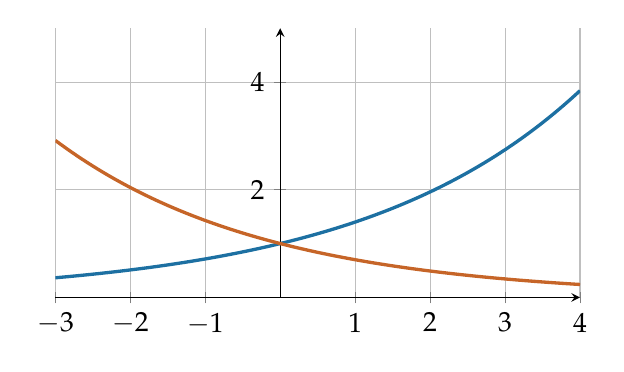
\begin{tikzpicture}\begin{axis}[width=.68\textwidth,height=5cm,axis lines=middle,xmin=-3,xmax=4,ymin=0,ymax=5,grid=major]\addplot[Blue,very thick,samples=100,domain=-3:4]{1.4^x};\addplot[Orange,very thick,samples=100,domain=-3:4]{.7^x};\end{axis}\end{tikzpicture}\end{center}
\end{activite}
\enseignant{La lecture graphique situe l'intersection vers $x\approx3{,}5$. Avant ce rang $g$ domine ; après, $f$ domine. Une valeur approchée est attendue. Faire verbaliser la donnée qui déclenche le choix de méthode.}

\begin{traceecrite}Lire $f(x)$ consiste à partir de $x$ vers la courbe puis vers l'axe des ordonnées. Chercher un antécédent de $y$ consiste à partir de $y$ vers la courbe puis vers l'axe des abscisses.\end{traceecrite}

\begin{exemple}
Reprendre les données de l'activité et rédiger la solution dans l'ordre : définition des objets, propriété utilisée, calcul exact ou approché, puis phrase de réponse. La réponse modèle figure dans l'édition enseignant.
\end{exemple}
\enseignant{La lecture graphique situe l'intersection vers $x\approx3{,}5$. Avant ce rang $g$ domine ; après, $f$ domine. Une valeur approchée est attendue.}

\begin{exercice}[-- essentiel]
\begin{enumerate}\item Simplifier $3^{x+3}\div3^x$ et $(2^x)^3$.\item Étudier le sens de variation de $f(x)=3\times1{,}03^x$ et $g(x)=-3\times0{,}8^x$.\item Une valeur initiale de $1550$ augmente de $3\,\%$ par an. Donner le modèle et calculer la valeur après $6$ ans.\end{enumerate}
\end{exercice}
\enseignant{$3^3$ et $2^{3x}$. $f$ est croissante ; $0{,}8^x$ est décroissante et le coefficient négatif rend $g$ croissante. Le modèle est $V(t)=1550\times\left(1+\dfrac{3}{100}\right)^t$.}

\manuelref{Calao, p. 52, n° 31 à 36}
\ExoSession{11}

\begin{dm}Reprendre l'exercice d'entraînement 2 avec les données suivantes : remplacer la donnée initiale par $175$ et le taux ou la raison par $7$. Rédiger en quatre lignes : données, formule, calcul, conclusion.\end{dm}
\enseignant{La correction dépend de l'exercice repris. Vérifier surtout la cohérence du modèle, le nombre d'itérations, l'arrondi et la phrase de conclusion.}

\begin{sortie}Sur une demi-feuille : écrire la règle principale de la séance, traiter un exemple très court et indiquer son degré de confiance de 1 à 4. Question(s) essentielle(s) du jour : 1, 2 et 3.\end{sortie}

\ifprof
\begin{methode}
\textbf{Conduite en 1 h :} 7 min d'automatismes ; 10 min de mise en commun et trace ; 28 min d'exercices essentiels ; 5 min de correction ; 3 min de billet de sortie.\\
\textbf{Conduite en 2 h :} ajouter 20 min de recherche de l'activité, 20 min d'institutionnalisation, un second exercice autonome et 10 min de correction comparée.\\
\textbf{Différenciation :} fournir aux élèves fragiles une fiche à quatre cases (données, modèle, calcul, conclusion). Demander aux élèves rapides de produire un contre-exemple, une justification ou une seconde méthode.
\end{methode}
\fi
\sessionheader{12}{05/11/2026}{B : 1 h -- C : 2 h}{Équations exponentielles simples}{Fonctions exponentielles}
\begin{objectifs}\begin{itemize}\item Résoudre avec une même base.\item Approcher une solution.\item Vérifier la vraisemblance.\end{itemize}\end{objectifs}
\begin{automatismes}\begin{enumerate}\item Calculer $5\,\%$ de $160$. \rep{$8$}\item Calculer $2^1\times2^3$. \rep{$2^4$}\item Écrire $5^{-2}$ sous forme de fraction. \rep{$\dfrac1{25}$}\item La fonction $x\mapsto0{,}7^x$ est-elle croissante ? \rep{Non, elle est décroissante.}\item Comparer $1{,}04^3$ et $1{,}04^7$. \rep{$1{,}04^3<1{,}04^7$}\end{enumerate}\end{automatismes}
\begin{prerequis}Relire la dernière trace écrite et savoir effectuer les calculs élémentaires mobilisés aujourd'hui. Avant l'activité, faire reformuler les mots-clés : résoudre avec une même base et approcher une solution.\end{prerequis}

\begin{activite}
Résoudre $4^x=64$, $9^x=\dfrac13$ et $1{,}12^x=2$ : d'abord par même base lorsque c'est possible, puis numériquement pour la dernière. Encadrer la dernière solution entre deux entiers.

\end{activite}
\enseignant{$x=3$ ; $9^x=3^{-1}$ donc $2x=-1$ et $x=-\dfrac12$ ; enfin $x\approx6{,}12$, entre $6$ et $7$. Faire verbaliser la donnée qui déclenche le choix de méthode.}

\begin{traceecrite}Pour résoudre $a^x=b$ : utiliser une même base quand c'est possible ; sinon encadrer ou utiliser un outil numérique. Vérifier que $b>0$.\end{traceecrite}

\begin{exemple}
Reprendre les données de l'activité et rédiger la solution dans l'ordre : définition des objets, propriété utilisée, calcul exact ou approché, puis phrase de réponse. La réponse modèle figure dans l'édition enseignant.
\end{exemple}
\enseignant{$x=3$ ; $9^x=3^{-1}$ donc $2x=-1$ et $x=-\dfrac12$ ; enfin $x\approx6{,}12$, entre $6$ et $7$.}

\begin{exercice}[-- essentiel]
\begin{enumerate}\item Simplifier $3^{x+4}\div3^x$ et $(2^x)^3$.\item Étudier le sens de variation de $f(x)=4\times1{,}04^x$ et $g(x)=-4\times0{,}8^x$.\item Une valeur initiale de $1600$ augmente de $4\,\%$ par an. Donner le modèle et calculer la valeur après $6$ ans.\end{enumerate}
\end{exercice}
\enseignant{$3^4$ et $2^{3x}$. $f$ est croissante ; $0{,}8^x$ est décroissante et le coefficient négatif rend $g$ croissante. Le modèle est $V(t)=1600\times\left(1+\dfrac{4}{100}\right)^t$.}

\manuelref{Calao, p. 52, n° 37--38, puis p. 54, n° 45--46}
\ExoSession{12}

\begin{dm}Reprendre l'exercice d'entraînement 3 avec les données suivantes : remplacer la donnée initiale par $180$ et le taux ou la raison par $2$. Rédiger en quatre lignes : données, formule, calcul, conclusion.\end{dm}
\enseignant{La correction dépend de l'exercice repris. Vérifier surtout la cohérence du modèle, le nombre d'itérations, l'arrondi et la phrase de conclusion.}

\begin{sortie}Sur une demi-feuille : écrire la règle principale de la séance, traiter un exemple très court et indiquer son degré de confiance de 1 à 4. Question(s) essentielle(s) du jour : 1 et 2.\end{sortie}

\ifprof
\begin{methode}
\textbf{Conduite en 1 h :} 7 min d'automatismes ; 10 min de mise en commun et trace ; 28 min d'exercices essentiels ; 5 min de correction ; 3 min de billet de sortie.\\
\textbf{Conduite en 2 h :} ajouter 20 min de recherche de l'activité, 20 min d'institutionnalisation, un second exercice autonome et 10 min de correction comparée.\\
\textbf{Différenciation :} fournir aux élèves fragiles une fiche à quatre cases (données, modèle, calcul, conclusion). Demander aux élèves rapides de produire un contre-exemple, une justification ou une seconde méthode.
\end{methode}
\fi
\sessionheader{13}{10/11/2026}{B : 2 h -- C : 1 h}{Modélisation par une fonction exponentielle}{Fonctions exponentielles}
\begin{objectifs}\begin{itemize}\item Construire un modèle exponentiel.\item Identifier les paramètres.\item Prévoir et interpréter.\end{itemize}\end{objectifs}
\begin{automatismes}\begin{enumerate}\item Écrire le coefficient multiplicateur d'une hausse de $10\,\%$. \rep{$1+\dfrac{10}{100}=1,10$}\item Écrire $5^{-2}$ sous forme de fraction. \rep{$\dfrac1{25}$}\item La fonction $x\mapsto0{,}7^x$ est-elle croissante ? \rep{Non, elle est décroissante.}\item Comparer $1{,}04^3$ et $1{,}04^7$. \rep{$1{,}04^3<1{,}04^7$}\item Calculer $2^2\times2^3$. \rep{$2^5$}\end{enumerate}\end{automatismes}
\begin{prerequis}Relire la dernière trace écrite et savoir effectuer les calculs élémentaires mobilisés aujourd'hui. Avant l'activité, faire reformuler les mots-clés : construire un modèle exponentiel et identifier les paramètres.\end{prerequis}

\begin{activite}
Une application compte $12\,000$ utilisateurs au lancement et sa fréquentation augmente de $9\,\%$ par mois. Construire $f(t)$, calculer $f(6)$, puis déterminer numériquement quand elle dépassera $25\,000$ utilisateurs.
\begin{center}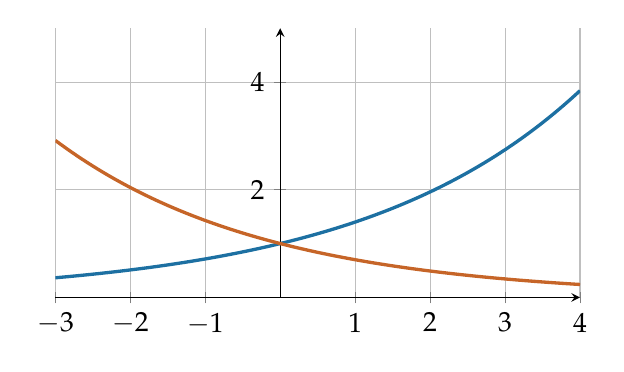
\begin{tikzpicture}\begin{axis}[width=.68\textwidth,height=5cm,axis lines=middle,xmin=-3,xmax=4,ymin=0,ymax=5,grid=major]\addplot[Blue,very thick,samples=100,domain=-3:4]{1.4^x};\addplot[Orange,very thick,samples=100,domain=-3:4]{.7^x};\end{axis}\end{tikzpicture}\end{center}
\end{activite}
\enseignant{$f(t)=12\,000\times1{,}09^t$, $f(6)\approx20\,126$. Le seuil est dépassé à partir du neuvième mois. Faire verbaliser la donnée qui déclenche le choix de méthode.}

\begin{traceecrite}Une évolution relative constante de coefficient $q$ se modélise par $f(t)=V_0q^t$. $V_0$ est la valeur initiale et $q$ le coefficient par unité de temps.\end{traceecrite}

\begin{exemple}
Reprendre les données de l'activité et rédiger la solution dans l'ordre : définition des objets, propriété utilisée, calcul exact ou approché, puis phrase de réponse. La réponse modèle figure dans l'édition enseignant.
\end{exemple}
\enseignant{$f(t)=12\,000\times1{,}09^t$, $f(6)\approx20\,126$. Le seuil est dépassé à partir du neuvième mois.}

\begin{exercice}[-- essentiel]
\begin{enumerate}\item Simplifier $3^{x+5}\div3^x$ et $(2^x)^3$.\item Étudier le sens de variation de $f(x)=5\times1{,}05^x$ et $g(x)=-5\times0{,}8^x$.\item Une valeur initiale de $1650$ augmente de $5\,\%$ par an. Donner le modèle et calculer la valeur après $6$ ans.\end{enumerate}
\end{exercice}
\enseignant{$3^5$ et $2^{3x}$. $f$ est croissante ; $0{,}8^x$ est décroissante et le coefficient négatif rend $g$ croissante. Le modèle est $V(t)=1650\times\left(1+\dfrac{5}{100}\right)^t$.}

\manuelref{Calao, p. 50, n° 20 à 25, puis p. 53, n° 41}
\ExoSession{13}

\begin{dm}Reprendre l'exercice d'entraînement 2 avec les données suivantes : remplacer la donnée initiale par $185$ et le taux ou la raison par $3$. Rédiger en quatre lignes : données, formule, calcul, conclusion.\end{dm}
\enseignant{La correction dépend de l'exercice repris. Vérifier surtout la cohérence du modèle, le nombre d'itérations, l'arrondi et la phrase de conclusion.}

\begin{sortie}Sur une demi-feuille : écrire la règle principale de la séance, traiter un exemple très court et indiquer son degré de confiance de 1 à 4. Question(s) essentielle(s) du jour : 1, 2 et 3.\end{sortie}

\ifprof
\begin{methode}
\textbf{Conduite en 1 h :} 7 min d'automatismes ; 10 min de mise en commun et trace ; 28 min d'exercices essentiels ; 5 min de correction ; 3 min de billet de sortie.\\
\textbf{Conduite en 2 h :} ajouter 20 min de recherche de l'activité, 20 min d'institutionnalisation, un second exercice autonome et 10 min de correction comparée.\\
\textbf{Différenciation :} fournir aux élèves fragiles une fiche à quatre cases (données, modèle, calcul, conclusion). Demander aux élèves rapides de produire un contre-exemple, une justification ou une seconde méthode.
\end{methode}
\fi
\sessionheader{14}{12/11/2026}{B : 1 h -- C : 2 h}{Bilan et évaluation du chapitre}{Fonctions exponentielles}
\begin{objectifs}\begin{itemize}\item Mobiliser les acquis du chapitre.\item Rédiger une modélisation.\item Corriger une erreur.\end{itemize}\end{objectifs}
\begin{automatismes}\begin{enumerate}\item Réduire $3x+3-x+2$. \rep{$2x+5$}\item La fonction $x\mapsto0{,}7^x$ est-elle croissante ? \rep{Non, elle est décroissante.}\item Comparer $1{,}04^3$ et $1{,}04^7$. \rep{$1{,}04^3<1{,}04^7$}\item Calculer $2^4\times2^3$. \rep{$2^7$}\item Écrire $5^{-2}$ sous forme de fraction. \rep{$\dfrac1{25}$}\end{enumerate}\end{automatismes}
\begin{prerequis}Relire la dernière trace écrite et savoir effectuer les calculs élémentaires mobilisés aujourd'hui. Avant l'activité, faire reformuler les mots-clés : mobiliser les acquis du chapitre et rédiger une modélisation.\end{prerequis}

\begin{activite}
À partir de quatre productions d'élèves, repérer et corriger : confusion taux/coefficient, propriété de puissances fausse, erreur de sens de variation et conclusion sans unité.

\end{activite}
\enseignant{La correction doit nommer l'erreur, écrire la règle correcte, reprendre le calcul et conclure dans le contexte. Faire verbaliser la donnée qui déclenche le choix de méthode.}

\begin{traceecrite}Pour valider un modèle exponentiel : identifier $V_0$ et $q$, calculer avec les unités, vérifier l'ordre de grandeur et interpréter le résultat.\end{traceecrite}

\begin{exemple}
Reprendre les données de l'activité et rédiger la solution dans l'ordre : définition des objets, propriété utilisée, calcul exact ou approché, puis phrase de réponse. La réponse modèle figure dans l'édition enseignant.
\end{exemple}
\enseignant{La correction doit nommer l'erreur, écrire la règle correcte, reprendre le calcul et conclure dans le contexte.}

\begin{exercice}[-- essentiel]
\begin{enumerate}\item Simplifier $3^{x+6}\div3^x$ et $(2^x)^3$.\item Étudier le sens de variation de $f(x)=6\times1{,}06^x$ et $g(x)=-6\times0{,}8^x$.\item Une valeur initiale de $1700$ augmente de $6\,\%$ par an. Donner le modèle et calculer la valeur après $6$ ans.\end{enumerate}
\end{exercice}
\enseignant{$3^6$ et $2^{3x}$. $f$ est croissante ; $0{,}8^x$ est décroissante et le coefficient négatif rend $g$ croissante. Le modèle est $V(t)=1700\times\left(1+\dfrac{6}{100}\right)^t$.}

\manuelref{Calao, p. 54, n° 47 à 58}
\ExoSession{14}

\begin{dm}Reprendre l'exercice d'entraînement 3 avec les données suivantes : remplacer la donnée initiale par $190$ et le taux ou la raison par $4$. Rédiger en quatre lignes : données, formule, calcul, conclusion.\end{dm}
\enseignant{La correction dépend de l'exercice repris. Vérifier surtout la cohérence du modèle, le nombre d'itérations, l'arrondi et la phrase de conclusion.}

\begin{sortie}Sur une demi-feuille : écrire la règle principale de la séance, traiter un exemple très court et indiquer son degré de confiance de 1 à 4. Question(s) essentielle(s) du jour : 1 et 2.\end{sortie}

\ifprof
\begin{methode}
\textbf{Conduite en 1 h :} 7 min d'automatismes ; 10 min de mise en commun et trace ; 28 min d'exercices essentiels ; 5 min de correction ; 3 min de billet de sortie.\\
\textbf{Conduite en 2 h :} ajouter 20 min de recherche de l'activité, 20 min d'institutionnalisation, un second exercice autonome et 10 min de correction comparée.\\
\textbf{Différenciation :} fournir aux élèves fragiles une fiche à quatre cases (données, modèle, calcul, conclusion). Demander aux élèves rapides de produire un contre-exemple, une justification ou une seconde méthode.
\end{methode}
\fi


\chapter{Fonction logarithme décimal}
\competences{passer d'une écriture exponentielle à une écriture logarithmique, résoudre, modéliser}
\section{Cours de référence}
\begin{retenir}
Pour tout $b>0$, $\log(b)$ est l'unique réel $x$ tel que $10^x=b$. Ainsi $\log(10^x)=x$ et, pour $b>0$, $10^{\log(b)}=b$. La fonction $\log$ est définie sur $]0,+\infty[$ et elle est strictement croissante.
\end{retenir}

\begin{center}
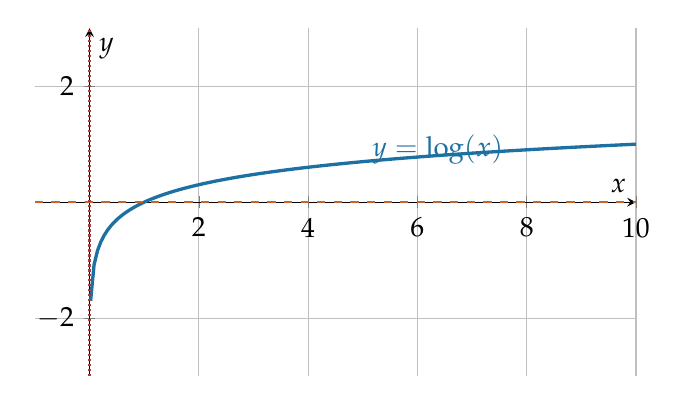
\begin{tikzpicture}
\begin{axis}[width=.76\textwidth,height=6cm,axis lines=middle,xmin=-1,xmax=10,ymin=-3,ymax=3,grid=major,xlabel={$x$},ylabel={$y$}]
\addplot[Blue,very thick,samples=160,domain=.02:10]{ln(x)/ln(10)};
\addplot[Orange,dashed,thick,domain=-1:10]{0};
\addplot[Red,densely dotted,thick] coordinates {(0,-3)(0,3)};
\node[anchor=west,Blue] at (axis cs:5,.9) {$y=\log(x)$};
\end{axis}
\end{tikzpicture}
\end{center}

Pour $a>0$, $b>0$ et tout entier naturel $n$ :
\[
\log(ab)=\log(a)+\log(b),\qquad
\log\!\left(\frac{a}{b}\right)=\log(a)-\log(b),\qquad
\log(a^n)=n\log(a).
\]

\begin{erreur}
$\log(a+b)$ ne se simplifie pas. Avant tout calcul logarithmique, vérifier que chaque argument est strictement positif.
\end{erreur}

\begin{methode}
Pour résoudre $a^x=b$, avec $a>0$, $a\neq1$ et $b>0$, on prend le logarithme : $x\log(a)=\log(b)$, donc $x=\dfrac{\log(b)}{\log(a)}$.
\end{methode}

\begin{exemple}
Résoudre $1{,}08^x=2$ revient à écrire $x=\dfrac{\log(2)}{\log(1{,}08)}\approx9{,}01$. Une valeur multipliée chaque année par $1{,}08$ double donc après un peu plus de neuf ans.
\end{exemple}

Comme $\log$ est croissante, pour $a,b>0$, $a<b$ équivaut à $\log(a)<\log(b)$. Pour $a>1$, $a^x<b$ équivaut à $x<\dfrac{\log b}{\log a}$ ; lorsque $0<a<1$, le sens de l'inégalité s'inverse.

\sessionheader{15}{17/11/2026}{B : 2 h -- C : 1 h}{Définition du logarithme décimal}{Fonction logarithme décimal}
\begin{objectifs}\begin{itemize}\item Relier puissance de 10 et logarithme.\item Calculer des valeurs usuelles.\item Utiliser la calculatrice.\end{itemize}\end{objectifs}
\begin{automatismes}\begin{enumerate}\item Calculer $20\,\%$ de $80$. \rep{$16$}\item Donner le domaine de $\log$. \rep{$]0,+\infty[$}\item Calculer $\log(10^4)$. \rep{$4$}\item Résoudre $10^x=0{,}01$. \rep{$x=-2$}\item Développer $\log(3b)$, $b>0$. \rep{$\log3+\log b$}\end{enumerate}\end{automatismes}
\begin{prerequis}Relire la dernière trace écrite et savoir effectuer les calculs élémentaires mobilisés aujourd'hui. Avant l'activité, faire reformuler les mots-clés : relier puissance de 10 et logarithme et calculer des valeurs usuelles.\end{prerequis}

\begin{activite}
Compléter les couples $10^x=b$ et $x=\log(b)$ pour $b=0{,}001;0{,}1;1;10;1\,000$. Puis utiliser la calculatrice pour $b=7$.

\end{activite}
\enseignant{Les logarithmes sont $-3,-1,0,1,3$ ; $\log(7)\approx0{,}8451$. Faire verbaliser la donnée qui déclenche le choix de méthode.}

\begin{traceecrite}Pour $b>0$, $\log(b)$ est l'unique solution de $10^x=b$. En particulier $\log(1)=0$, $\log(10)=1$ et $\log(100)=2$.\end{traceecrite}

\begin{exemple}
Reprendre les données de l'activité et rédiger la solution dans l'ordre : définition des objets, propriété utilisée, calcul exact ou approché, puis phrase de réponse. La réponse modèle figure dans l'édition enseignant.
\end{exemple}
\enseignant{Les logarithmes sont $-3,-1,0,1,3$ ; $\log(7)\approx0{,}8451$.}

\begin{exercice}[-- essentiel]
\begin{enumerate}\item Calculer $\log(10^2)$ et $\log(10^{-2})$.\item Développer $\log\!\left(\dfrac{100a^2}{b}\right)$ pour $a,b>0$.\item Résoudre $2^x=22$ et donner une valeur approchée au centième.\end{enumerate}
\end{exercice}
\enseignant{$2$ et $-2$. L'expression vaut $2+2\log(a)-\log(b)$. Enfin $x=\dfrac{\log(22)}{\log(2)}$.}

\manuelref{Calao, cours p. 64--69 ; exercices p. 70, n° 1 à 5}
\CalaoSession{15}

\begin{dm}Reprendre l'exercice d'entraînement 2 avec les données suivantes : remplacer la donnée initiale par $195$ et le taux ou la raison par $5$. Rédiger en quatre lignes : données, formule, calcul, conclusion.\end{dm}
\enseignant{La correction dépend de l'exercice repris. Vérifier surtout la cohérence du modèle, le nombre d'itérations, l'arrondi et la phrase de conclusion.}

\begin{sortie}Sur une demi-feuille : écrire la règle principale de la séance, traiter un exemple très court et indiquer son degré de confiance de 1 à 4. Question(s) essentielle(s) du jour : 1, 2 et 3.\end{sortie}

\ifprof
\begin{methode}
\textbf{Conduite en 1 h :} 7 min d'automatismes ; 10 min de mise en commun et trace ; 28 min d'exercices essentiels ; 5 min de correction ; 3 min de billet de sortie.\\
\textbf{Conduite en 2 h :} ajouter 20 min de recherche de l'activité, 20 min d'institutionnalisation, un second exercice autonome et 10 min de correction comparée.\\
\textbf{Différenciation :} fournir aux élèves fragiles une fiche à quatre cases (données, modèle, calcul, conclusion). Demander aux élèves rapides de produire un contre-exemple, une justification ou une seconde méthode.
\end{methode}
\fi
\sessionheader{16}{19/11/2026}{B : 1 h -- C : 2 h}{Sens de variation et représentation}{Fonction logarithme décimal}
\begin{objectifs}\begin{itemize}\item Connaître le domaine.\item Utiliser la croissance.\item Lire la courbe.\end{itemize}\end{objectifs}
\begin{automatismes}\begin{enumerate}\item Écrire le coefficient multiplicateur d'une hausse de $25\,\%$. \rep{$1+\dfrac{25}{100}=1,25$}\item Calculer $\log(10^0)$. \rep{$0$}\item Résoudre $10^x=0{,}01$. \rep{$x=-2$}\item Développer $\log(3b)$, $b>0$. \rep{$\log3+\log b$}\item Donner le domaine de $\log$. \rep{$]0,+\infty[$}\end{enumerate}\end{automatismes}
\begin{prerequis}Relire la dernière trace écrite et savoir effectuer les calculs élémentaires mobilisés aujourd'hui. Avant l'activité, faire reformuler les mots-clés : connaître le domaine et utiliser la croissance.\end{prerequis}

\begin{activite}
Tracer $y=10^x$ et la droite $y=x$, puis obtenir la courbe du logarithme par symétrie. En déduire son domaine, son sens de variation et l'asymptote.
\begin{center}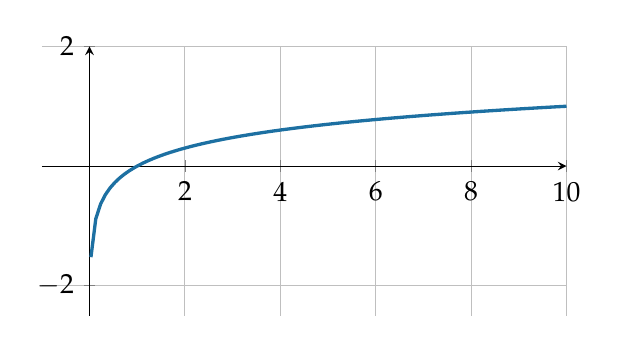
\begin{tikzpicture}\begin{axis}[width=.68\textwidth,height=5cm,axis lines=middle,xmin=-1,xmax=10,ymin=-2.5,ymax=2,grid=major]\addplot[Blue,very thick,samples=100,domain=.03:10]{ln(x)/ln(10)};\end{axis}\end{tikzpicture}\end{center}
\end{activite}
\enseignant{Le logarithme est la fonction réciproque de $10^x$ : domaine $]0,+\infty[$, croissance stricte, asymptote $x=0$. Faire verbaliser la donnée qui déclenche le choix de méthode.}

\begin{traceecrite}La fonction $\log$ est définie sur $]0,+\infty[$, strictement croissante, et sa courbe admet $x=0$ comme asymptote verticale.\end{traceecrite}

\begin{exemple}
Reprendre les données de l'activité et rédiger la solution dans l'ordre : définition des objets, propriété utilisée, calcul exact ou approché, puis phrase de réponse. La réponse modèle figure dans l'édition enseignant.
\end{exemple}
\enseignant{Le logarithme est la fonction réciproque de $10^x$ : domaine $]0,+\infty[$, croissance stricte, asymptote $x=0$.}

\begin{exercice}[-- essentiel]
\begin{enumerate}\item Calculer $\log(10^3)$ et $\log(10^{-3})$.\item Développer $\log\!\left(\dfrac{100a^2}{b}\right)$ pour $a,b>0$.\item Résoudre $3^x=23$ et donner une valeur approchée au centième.\end{enumerate}
\end{exercice}
\enseignant{$3$ et $-3$. L'expression vaut $2+2\log(a)-\log(b)$. Enfin $x=\dfrac{\log(23)}{\log(3)}$.}

\manuelref{Calao, cours p. 64--69 ; exercices p. 70, n° 6 à 10}
\CalaoSession{16}

\begin{dm}Reprendre l'exercice d'entraînement 3 avec les données suivantes : remplacer la donnée initiale par $200$ et le taux ou la raison par $6$. Rédiger en quatre lignes : données, formule, calcul, conclusion.\end{dm}
\enseignant{La correction dépend de l'exercice repris. Vérifier surtout la cohérence du modèle, le nombre d'itérations, l'arrondi et la phrase de conclusion.}

\begin{sortie}Sur une demi-feuille : écrire la règle principale de la séance, traiter un exemple très court et indiquer son degré de confiance de 1 à 4. Question(s) essentielle(s) du jour : 1 et 2.\end{sortie}

\ifprof
\begin{methode}
\textbf{Conduite en 1 h :} 7 min d'automatismes ; 10 min de mise en commun et trace ; 28 min d'exercices essentiels ; 5 min de correction ; 3 min de billet de sortie.\\
\textbf{Conduite en 2 h :} ajouter 20 min de recherche de l'activité, 20 min d'institutionnalisation, un second exercice autonome et 10 min de correction comparée.\\
\textbf{Différenciation :} fournir aux élèves fragiles une fiche à quatre cases (données, modèle, calcul, conclusion). Demander aux élèves rapides de produire un contre-exemple, une justification ou une seconde méthode.
\end{methode}
\fi
\sessionheader{17}{24/11/2026}{B : 2 h -- C : 1 h}{Propriétés algébriques}{Fonction logarithme décimal}
\begin{objectifs}\begin{itemize}\item Développer ou condenser des logarithmes.\item Vérifier les conditions.\item Éviter les fausses propriétés.\end{itemize}\end{objectifs}
\begin{automatismes}\begin{enumerate}\item Réduire $3x+6-x+2$. \rep{$2x+8$}\item Résoudre $10^x=0{,}01$. \rep{$x=-2$}\item Développer $\log(3b)$, $b>0$. \rep{$\log3+\log b$}\item Donner le domaine de $\log$. \rep{$]0,+\infty[$}\item Calculer $\log(10^1)$. \rep{$1$}\end{enumerate}\end{automatismes}
\begin{prerequis}Relire la dernière trace écrite et savoir effectuer les calculs élémentaires mobilisés aujourd'hui. Avant l'activité, faire reformuler les mots-clés : développer ou condenser des logarithmes et vérifier les conditions.\end{prerequis}

\begin{activite}
À partir de $10^2\times10^3=10^5$, conjecturer $\log(ab)=\log a+\log b$. Tester numériquement avec $a=2,b=5$, puis expliquer pourquoi $a,b$ doivent être positifs.

\end{activite}
\enseignant{$\log(2)+\log(5)=\log(10)=1$. Le logarithme n'est défini que pour un argument strictement positif. Faire verbaliser la donnée qui déclenche le choix de méthode.}

\begin{traceecrite}Pour $a,b>0$, $\log(ab)=\log a+\log b$ et $\log\!\left(\dfrac ab\right)=\log a-\log b$. De plus $\log(a^n)=n\log a$.\end{traceecrite}

\begin{exemple}
Reprendre les données de l'activité et rédiger la solution dans l'ordre : définition des objets, propriété utilisée, calcul exact ou approché, puis phrase de réponse. La réponse modèle figure dans l'édition enseignant.
\end{exemple}
\enseignant{$\log(2)+\log(5)=\log(10)=1$. Le logarithme n'est défini que pour un argument strictement positif.}

\begin{exercice}[-- essentiel]
\begin{enumerate}\item Calculer $\log(10^4)$ et $\log(10^{-4})$.\item Développer $\log\!\left(\dfrac{100a^2}{b}\right)$ pour $a,b>0$.\item Résoudre $4^x=24$ et donner une valeur approchée au centième.\end{enumerate}
\end{exercice}
\enseignant{$4$ et $-4$. L'expression vaut $2+2\log(a)-\log(b)$. Enfin $x=\dfrac{\log(24)}{\log(4)}$.}

\manuelref{Calao, cours p. 66--69 ; exercices p. 72, n° 20 à 23}
\CalaoSession{17}

\begin{dm}Reprendre l'exercice d'entraînement 2 avec les données suivantes : remplacer la donnée initiale par $205$ et le taux ou la raison par $7$. Rédiger en quatre lignes : données, formule, calcul, conclusion.\end{dm}
\enseignant{La correction dépend de l'exercice repris. Vérifier surtout la cohérence du modèle, le nombre d'itérations, l'arrondi et la phrase de conclusion.}

\begin{sortie}Sur une demi-feuille : écrire la règle principale de la séance, traiter un exemple très court et indiquer son degré de confiance de 1 à 4. Question(s) essentielle(s) du jour : 1, 2 et 3.\end{sortie}

\ifprof
\begin{methode}
\textbf{Conduite en 1 h :} 7 min d'automatismes ; 10 min de mise en commun et trace ; 28 min d'exercices essentiels ; 5 min de correction ; 3 min de billet de sortie.\\
\textbf{Conduite en 2 h :} ajouter 20 min de recherche de l'activité, 20 min d'institutionnalisation, un second exercice autonome et 10 min de correction comparée.\\
\textbf{Différenciation :} fournir aux élèves fragiles une fiche à quatre cases (données, modèle, calcul, conclusion). Demander aux élèves rapides de produire un contre-exemple, une justification ou une seconde méthode.
\end{methode}
\fi
\sessionheader{18}{26/11/2026}{B : 1 h -- C : 2 h}{Résoudre $10^x=b$}{Fonction logarithme décimal}
\begin{objectifs}\begin{itemize}\item Résoudre $10^x=b$.\item Encadrer une solution.\item Interpréter un ordre de grandeur.\end{itemize}\end{objectifs}
\begin{automatismes}\begin{enumerate}\item Calculer $5\,\%$ de $140$. \rep{$7$}\item Développer $\log(3b)$, $b>0$. \rep{$\log3+\log b$}\item Donner le domaine de $\log$. \rep{$]0,+\infty[$}\item Calculer $\log(10^2)$. \rep{$2$}\item Résoudre $10^x=0{,}01$. \rep{$x=-2$}\end{enumerate}\end{automatismes}
\begin{prerequis}Relire la dernière trace écrite et savoir effectuer les calculs élémentaires mobilisés aujourd'hui. Avant l'activité, faire reformuler les mots-clés : résoudre $10^x=b$ et encadrer une solution.\end{prerequis}

\begin{activite}
Un appareil mesure des intensités $b=0{,}04;3{,}2;850$. Pour chaque valeur, résoudre $10^x=b$, donner $x$ au centième et vérifier en calculant $10^x$.

\end{activite}
\enseignant{$x=\log(b)$ : environ $-1{,}40$, $0{,}51$ et $2{,}93$. Faire verbaliser la donnée qui déclenche le choix de méthode.}

\begin{traceecrite}L'équation $10^x=b$ n'a de solution que si $b>0$ ; cette solution est $x=\log(b)$.\end{traceecrite}

\begin{exemple}
Reprendre les données de l'activité et rédiger la solution dans l'ordre : définition des objets, propriété utilisée, calcul exact ou approché, puis phrase de réponse. La réponse modèle figure dans l'édition enseignant.
\end{exemple}
\enseignant{$x=\log(b)$ : environ $-1{,}40$, $0{,}51$ et $2{,}93$.}

\begin{exercice}[-- essentiel]
\begin{enumerate}\item Calculer $\log(10^5)$ et $\log(10^{-5})$.\item Développer $\log\!\left(\dfrac{100a^2}{b}\right)$ pour $a,b>0$.\item Résoudre $5^x=25$ et donner une valeur approchée au centième.\end{enumerate}
\end{exercice}
\enseignant{$5$ et $-5$. L'expression vaut $2+2\log(a)-\log(b)$. Enfin $x=\dfrac{\log(25)}{\log(5)}$.}

\manuelref{Calao, p. 73, n° 30 à 32}
\CalaoSession{18}

\begin{dm}Reprendre l'exercice d'entraînement 3 avec les données suivantes : remplacer la donnée initiale par $210$ et le taux ou la raison par $2$. Rédiger en quatre lignes : données, formule, calcul, conclusion.\end{dm}
\enseignant{La correction dépend de l'exercice repris. Vérifier surtout la cohérence du modèle, le nombre d'itérations, l'arrondi et la phrase de conclusion.}

\begin{sortie}Sur une demi-feuille : écrire la règle principale de la séance, traiter un exemple très court et indiquer son degré de confiance de 1 à 4. Question(s) essentielle(s) du jour : 1 et 2.\end{sortie}

\ifprof
\begin{methode}
\textbf{Conduite en 1 h :} 7 min d'automatismes ; 10 min de mise en commun et trace ; 28 min d'exercices essentiels ; 5 min de correction ; 3 min de billet de sortie.\\
\textbf{Conduite en 2 h :} ajouter 20 min de recherche de l'activité, 20 min d'institutionnalisation, un second exercice autonome et 10 min de correction comparée.\\
\textbf{Différenciation :} fournir aux élèves fragiles une fiche à quatre cases (données, modèle, calcul, conclusion). Demander aux élèves rapides de produire un contre-exemple, une justification ou une seconde méthode.
\end{methode}
\fi
\sessionheader{19}{01/12/2026}{B : 2 h -- C : 1 h}{Résoudre $a^x=b$}{Fonction logarithme décimal}
\begin{objectifs}\begin{itemize}\item Résoudre $a^x=b$.\item Utiliser un quotient de logarithmes.\item Arrondir avec sens.\end{itemize}\end{objectifs}
\begin{automatismes}\begin{enumerate}\item Écrire le coefficient multiplicateur d'une hausse de $10\,\%$. \rep{$1+\dfrac{10}{100}=1,10$}\item Donner le domaine de $\log$. \rep{$]0,+\infty[$}\item Calculer $\log(10^3)$. \rep{$3$}\item Résoudre $10^x=0{,}01$. \rep{$x=-2$}\item Développer $\log(3b)$, $b>0$. \rep{$\log3+\log b$}\end{enumerate}\end{automatismes}
\begin{prerequis}Relire la dernière trace écrite et savoir effectuer les calculs élémentaires mobilisés aujourd'hui. Avant l'activité, faire reformuler les mots-clés : résoudre $a^x=b$ et utiliser un quotient de logarithmes.\end{prerequis}

\begin{activite}
Le nombre d'abonnés est multiplié par $1{,}15$ chaque mois. Déterminer au bout de combien de mois il aura triplé. Poser l'équation, la résoudre avec les logarithmes et interpréter l'arrondi.

\end{activite}
\enseignant{$1{,}15^n\geq3$ ; $\dfrac{\log3}{\log1{,}15}\approx7{,}86$. Il faut donc huit mois entiers. Faire verbaliser la donnée qui déclenche le choix de méthode.}

\begin{traceecrite}Pour $a>0$, $a\neq1$ et $b>0$, $a^x=b$ équivaut à $x=\dfrac{\log(b)}{\log(a)}$.\end{traceecrite}

\begin{exemple}
Reprendre les données de l'activité et rédiger la solution dans l'ordre : définition des objets, propriété utilisée, calcul exact ou approché, puis phrase de réponse. La réponse modèle figure dans l'édition enseignant.
\end{exemple}
\enseignant{$1{,}15^n\geq3$ ; $\dfrac{\log3}{\log1{,}15}\approx7{,}86$. Il faut donc huit mois entiers.}

\begin{exercice}[-- essentiel]
\begin{enumerate}\item Calculer $\log(10^6)$ et $\log(10^{-6})$.\item Développer $\log\!\left(\dfrac{100a^2}{b}\right)$ pour $a,b>0$.\item Résoudre $6^x=26$ et donner une valeur approchée au centième.\end{enumerate}
\end{exercice}
\enseignant{$6$ et $-6$. L'expression vaut $2+2\log(a)-\log(b)$. Enfin $x=\dfrac{\log(26)}{\log(6)}$.}

\manuelref{Calao, p. 74, n° 33 à 39}
\CalaoSession{19}

\begin{dm}Reprendre l'exercice d'entraînement 2 avec les données suivantes : remplacer la donnée initiale par $215$ et le taux ou la raison par $3$. Rédiger en quatre lignes : données, formule, calcul, conclusion.\end{dm}
\enseignant{La correction dépend de l'exercice repris. Vérifier surtout la cohérence du modèle, le nombre d'itérations, l'arrondi et la phrase de conclusion.}

\begin{sortie}Sur une demi-feuille : écrire la règle principale de la séance, traiter un exemple très court et indiquer son degré de confiance de 1 à 4. Question(s) essentielle(s) du jour : 1, 2 et 3.\end{sortie}

\ifprof
\begin{methode}
\textbf{Conduite en 1 h :} 7 min d'automatismes ; 10 min de mise en commun et trace ; 28 min d'exercices essentiels ; 5 min de correction ; 3 min de billet de sortie.\\
\textbf{Conduite en 2 h :} ajouter 20 min de recherche de l'activité, 20 min d'institutionnalisation, un second exercice autonome et 10 min de correction comparée.\\
\textbf{Différenciation :} fournir aux élèves fragiles une fiche à quatre cases (données, modèle, calcul, conclusion). Demander aux élèves rapides de produire un contre-exemple, une justification ou une seconde méthode.
\end{methode}
\fi
\sessionheader{20}{03/12/2026}{B : 1 h -- C : 2 h}{Équations $x^a=b$ et inégalités simples}{Fonction logarithme décimal}
\begin{objectifs}\begin{itemize}\item Résoudre une puissance inconnue.\item Traiter une inégalité.\item Tenir compte du domaine.\end{itemize}\end{objectifs}
\begin{automatismes}\begin{enumerate}\item Réduire $3x+9-x+2$. \rep{$2x+11$}\item Calculer $\log(10^4)$. \rep{$4$}\item Résoudre $10^x=0{,}01$. \rep{$x=-2$}\item Développer $\log(3b)$, $b>0$. \rep{$\log3+\log b$}\item Donner le domaine de $\log$. \rep{$]0,+\infty[$}\end{enumerate}\end{automatismes}
\begin{prerequis}Relire la dernière trace écrite et savoir effectuer les calculs élémentaires mobilisés aujourd'hui. Avant l'activité, faire reformuler les mots-clés : résoudre une puissance inconnue et traiter une inégalité.\end{prerequis}

\begin{activite}
Résoudre sur $[0,+\infty[$ : $x^3=40$, puis $x^4=16$. Résoudre ensuite $1{,}08^x<1{,}5$ et expliquer le rôle de la croissance.

\end{activite}
\enseignant{$x=\sqrt[3]{40}\approx3{,}42$ ; $x=2$ sur l'intervalle demandé ; $x<\dfrac{\log1{,}5}{\log1{,}08}\approx5{,}27$. Faire verbaliser la donnée qui déclenche le choix de méthode.}

\begin{traceecrite}Pour résoudre $x^n=b$, tenir compte du domaine et de la parité de $n$. Pour une inégalité exponentielle, le sens dépend de la croissance ou décroissance de la fonction.\end{traceecrite}

\begin{exemple}
Reprendre les données de l'activité et rédiger la solution dans l'ordre : définition des objets, propriété utilisée, calcul exact ou approché, puis phrase de réponse. La réponse modèle figure dans l'édition enseignant.
\end{exemple}
\enseignant{$x=\sqrt[3]{40}\approx3{,}42$ ; $x=2$ sur l'intervalle demandé ; $x<\dfrac{\log1{,}5}{\log1{,}08}\approx5{,}27$.}

\begin{exercice}[-- essentiel]
\begin{enumerate}\item Calculer $\log(10^2)$ et $\log(10^{-2})$.\item Développer $\log\!\left(\dfrac{100a^2}{b}\right)$ pour $a,b>0$.\item Résoudre $2^x=22$ et donner une valeur approchée au centième.\end{enumerate}
\end{exercice}
\enseignant{$2$ et $-2$. L'expression vaut $2+2\log(a)-\log(b)$. Enfin $x=\dfrac{\log(22)}{\log(2)}$.}

\manuelref{Calao, p. 75, n° 40 à 42}
\CalaoSession{20}

\begin{dm}Reprendre l'exercice d'entraînement 3 avec les données suivantes : remplacer la donnée initiale par $220$ et le taux ou la raison par $4$. Rédiger en quatre lignes : données, formule, calcul, conclusion.\end{dm}
\enseignant{La correction dépend de l'exercice repris. Vérifier surtout la cohérence du modèle, le nombre d'itérations, l'arrondi et la phrase de conclusion.}

\begin{sortie}Sur une demi-feuille : écrire la règle principale de la séance, traiter un exemple très court et indiquer son degré de confiance de 1 à 4. Question(s) essentielle(s) du jour : 1 et 2.\end{sortie}

\ifprof
\begin{methode}
\textbf{Conduite en 1 h :} 7 min d'automatismes ; 10 min de mise en commun et trace ; 28 min d'exercices essentiels ; 5 min de correction ; 3 min de billet de sortie.\\
\textbf{Conduite en 2 h :} ajouter 20 min de recherche de l'activité, 20 min d'institutionnalisation, un second exercice autonome et 10 min de correction comparée.\\
\textbf{Différenciation :} fournir aux élèves fragiles une fiche à quatre cases (données, modèle, calcul, conclusion). Demander aux élèves rapides de produire un contre-exemple, une justification ou une seconde méthode.
\end{methode}
\fi
\sessionheader{21}{08/12/2026}{B : 2 h -- C : 1 h}{Problèmes contextualisés}{Fonction logarithme décimal}
\begin{objectifs}\begin{itemize}\item Modéliser une situation.\item Choisir une équation.\item Conclure dans le contexte.\end{itemize}\end{objectifs}
\begin{automatismes}\begin{enumerate}\item Calculer $20\,\%$ de $60$. \rep{$12$}\item Résoudre $10^x=0{,}01$. \rep{$x=-2$}\item Développer $\log(3b)$, $b>0$. \rep{$\log3+\log b$}\item Donner le domaine de $\log$. \rep{$]0,+\infty[$}\item Calculer $\log(10^3)$. \rep{$3$}\end{enumerate}\end{automatismes}
\begin{prerequis}Relire la dernière trace écrite et savoir effectuer les calculs élémentaires mobilisés aujourd'hui. Avant l'activité, faire reformuler les mots-clés : modéliser une situation et choisir une équation.\end{prerequis}

\begin{activite}
Le niveau sonore est $L=10\log\!\left(\dfrac I{I_0}\right)$. Calculer $L$ lorsque $I=10^6I_0$. Puis déterminer le rapport $\dfrac I{I_0}$ pour $L=85$ dB.

\end{activite}
\enseignant{$L=60$ dB. Pour $85$ dB, $\log\!\left(\dfrac I{I_0}\right)=8{,}5$, donc $\dfrac I{I_0}=10^{8{,}5}\approx3{,}16\times10^8$. Faire verbaliser la donnée qui déclenche le choix de méthode.}

\begin{traceecrite}Dans un problème, définir la variable, poser l'équation, résoudre, contrôler le domaine et conclure avec l'unité. Une solution numérique sans interprétation est incomplète.\end{traceecrite}

\begin{exemple}
Reprendre les données de l'activité et rédiger la solution dans l'ordre : définition des objets, propriété utilisée, calcul exact ou approché, puis phrase de réponse. La réponse modèle figure dans l'édition enseignant.
\end{exemple}
\enseignant{$L=60$ dB. Pour $85$ dB, $\log\!\left(\dfrac I{I_0}\right)=8{,}5$, donc $\dfrac I{I_0}=10^{8{,}5}\approx3{,}16\times10^8$.}

\begin{exercice}[-- essentiel]
\begin{enumerate}\item Calculer $\log(10^3)$ et $\log(10^{-3})$.\item Développer $\log\!\left(\dfrac{100a^2}{b}\right)$ pour $a,b>0$.\item Résoudre $3^x=23$ et donner une valeur approchée au centième.\end{enumerate}
\end{exercice}
\enseignant{$3$ et $-3$. L'expression vaut $2+2\log(a)-\log(b)$. Enfin $x=\dfrac{\log(23)}{\log(3)}$.}

\manuelref{Calao, p. 74, n° 38--39, puis p. 75, n° 40 à 42}
\CalaoSession{21}

\begin{dm}Reprendre l'exercice d'entraînement 2 avec les données suivantes : remplacer la donnée initiale par $225$ et le taux ou la raison par $5$. Rédiger en quatre lignes : données, formule, calcul, conclusion.\end{dm}
\enseignant{La correction dépend de l'exercice repris. Vérifier surtout la cohérence du modèle, le nombre d'itérations, l'arrondi et la phrase de conclusion.}

\begin{sortie}Sur une demi-feuille : écrire la règle principale de la séance, traiter un exemple très court et indiquer son degré de confiance de 1 à 4. Question(s) essentielle(s) du jour : 1, 2 et 3.\end{sortie}

\ifprof
\begin{methode}
\textbf{Conduite en 1 h :} 7 min d'automatismes ; 10 min de mise en commun et trace ; 28 min d'exercices essentiels ; 5 min de correction ; 3 min de billet de sortie.\\
\textbf{Conduite en 2 h :} ajouter 20 min de recherche de l'activité, 20 min d'institutionnalisation, un second exercice autonome et 10 min de correction comparée.\\
\textbf{Différenciation :} fournir aux élèves fragiles une fiche à quatre cases (données, modèle, calcul, conclusion). Demander aux élèves rapides de produire un contre-exemple, une justification ou une seconde méthode.
\end{methode}
\fi
\sessionheader{22}{10/12/2026}{B : 1 h -- C : 2 h}{Bilan et évaluation}{Fonction logarithme décimal}
\begin{objectifs}\begin{itemize}\item Synthétiser les méthodes.\item Identifier les conditions.\item Remédier aux erreurs.\end{itemize}\end{objectifs}
\begin{automatismes}\begin{enumerate}\item Écrire le coefficient multiplicateur d'une hausse de $25\,\%$. \rep{$1+\dfrac{25}{100}=1,25$}\item Développer $\log(3b)$, $b>0$. \rep{$\log3+\log b$}\item Donner le domaine de $\log$. \rep{$]0,+\infty[$}\item Calculer $\log(10^4)$. \rep{$4$}\item Résoudre $10^x=0{,}01$. \rep{$x=-2$}\end{enumerate}\end{automatismes}
\begin{prerequis}Relire la dernière trace écrite et savoir effectuer les calculs élémentaires mobilisés aujourd'hui. Avant l'activité, faire reformuler les mots-clés : synthétiser les méthodes et identifier les conditions.\end{prerequis}

\begin{activite}
Réaliser une carte de méthodes : domaine ; propriétés ; équations $10^x=b$ ; équations $a^x=b$ ; inégalités. Associer à chaque branche une condition et un exemple.

\end{activite}
\enseignant{La carte doit notamment faire apparaître la positivité des arguments et la distinction entre base supérieure à $1$ ou comprise entre $0$ et $1$. Faire verbaliser la donnée qui déclenche le choix de méthode.}

\begin{traceecrite}Avant un calcul de logarithme : vérifier la positivité. Avant une comparaison : identifier le sens de variation. Avant une conclusion : contrôler la vraisemblance.\end{traceecrite}

\begin{exemple}
Reprendre les données de l'activité et rédiger la solution dans l'ordre : définition des objets, propriété utilisée, calcul exact ou approché, puis phrase de réponse. La réponse modèle figure dans l'édition enseignant.
\end{exemple}
\enseignant{La carte doit notamment faire apparaître la positivité des arguments et la distinction entre base supérieure à $1$ ou comprise entre $0$ et $1$.}

\begin{exercice}[-- essentiel]
\begin{enumerate}\item Calculer $\log(10^4)$ et $\log(10^{-4})$.\item Développer $\log\!\left(\dfrac{100a^2}{b}\right)$ pour $a,b>0$.\item Résoudre $4^x=24$ et donner une valeur approchée au centième.\end{enumerate}
\end{exercice}
\enseignant{$4$ et $-4$. L'expression vaut $2+2\log(a)-\log(b)$. Enfin $x=\dfrac{\log(24)}{\log(4)}$.}

\manuelref{Calao, p. 76 à 79}
\CalaoSession{22}

\begin{dm}Reprendre l'exercice d'entraînement 3 avec les données suivantes : remplacer la donnée initiale par $230$ et le taux ou la raison par $6$. Rédiger en quatre lignes : données, formule, calcul, conclusion.\end{dm}
\enseignant{La correction dépend de l'exercice repris. Vérifier surtout la cohérence du modèle, le nombre d'itérations, l'arrondi et la phrase de conclusion.}

\begin{sortie}Sur une demi-feuille : écrire la règle principale de la séance, traiter un exemple très court et indiquer son degré de confiance de 1 à 4. Question(s) essentielle(s) du jour : 1 et 2.\end{sortie}

\ifprof
\begin{methode}
\textbf{Conduite en 1 h :} 7 min d'automatismes ; 10 min de mise en commun et trace ; 28 min d'exercices essentiels ; 5 min de correction ; 3 min de billet de sortie.\\
\textbf{Conduite en 2 h :} ajouter 20 min de recherche de l'activité, 20 min d'institutionnalisation, un second exercice autonome et 10 min de correction comparée.\\
\textbf{Différenciation :} fournir aux élèves fragiles une fiche à quatre cases (données, modèle, calcul, conclusion). Demander aux élèves rapides de produire un contre-exemple, une justification ou une seconde méthode.
\end{methode}
\fi


\chapter{Fonction inverse}
\competences{déterminer un domaine, dériver, étudier un signe, dresser un tableau de variations, représenter}
\section{Cours de référence}
La fonction inverse est définie par $f(x)=\dfrac1x$ sur $\R\setminus\{0\}$.

\begin{center}
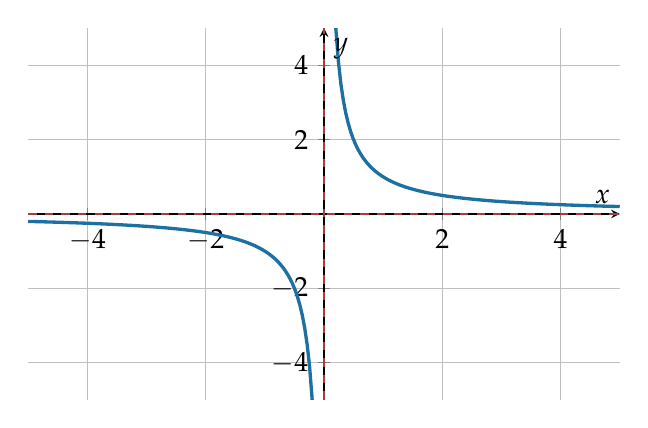
\begin{tikzpicture}
\begin{axis}[width=.75\textwidth,height=6.3cm,axis lines=middle,xmin=-5,xmax=5,ymin=-5,ymax=5,grid=major,xlabel={$x$},ylabel={$y$},unbounded coords=jump]
\addplot[Blue,very thick,samples=120,domain=-5:-.12]{1/x};
\addplot[Blue,very thick,samples=120,domain=.12:5]{1/x};
\addplot[Red,dashed,thick] coordinates {(0,-5)(0,5)};
\addplot[Red,dashed,thick] coordinates {(-5,0)(5,0)};
\end{axis}
\end{tikzpicture}
\end{center}

\begin{retenir}
$f'(x)=-\dfrac1{x^2}<0$ pour tout $x\neq0$. La fonction inverse est strictement décroissante sur chacun des intervalles $]-\infty,0[$ et $]0,+\infty[$. Les droites $x=0$ et $y=0$ sont des asymptotes.
\end{retenir}

\begin{erreur}
On ne peut pas écrire que la fonction inverse est décroissante « sur $\R\setminus\{0\}$ » sans préciser les deux intervalles. Par exemple $-1<1$ mais $f(-1)=-1<1=f(1)$, ce qui contreditrait la définition globale de la décroissance.
\end{erreur}

Pour une fonction $g(x)=P(x)+\dfrac{k}{x}$, on procède dans cet ordre : domaine ; dérivée ; mise au même dénominateur et factorisation ; signe de la dérivée ; variations ; limites ou comportement aux bornes ; points utiles ; représentation.

\begin{exemple}
Sur $]0,+\infty[$, $g(x)=x+\dfrac4x$ vérifie $g'(x)=1-\dfrac4{x^2}=\dfrac{(x-2)(x+2)}{x^2}$. Le dénominateur est positif ; $g'$ est négative sur $]0,2[$ puis positive sur $]2,+\infty[$. La fonction admet un minimum $g(2)=4$.
\end{exemple}

\sessionheader{23}{15/12/2026}{B : 2 h -- C : 1 h}{Définition et courbe de la fonction inverse}{Fonction inverse}
\begin{objectifs}\begin{itemize}\item Déterminer le domaine.\item Construire la courbe.\item Utiliser les symétries.\end{itemize}\end{objectifs}
\begin{automatismes}\begin{enumerate}\item Réduire $3x+5-x+2$. \rep{$2x+7$}\item Donner la valeur interdite de $\dfrac{x+1}{x}$. \rep{$x=0$}\item Calculer $\dfrac1{5}$ et $\dfrac1{-5}$. \rep{$\dfrac1{5}$ et $-\dfrac1{5}$}\item Dériver $3x^2-5x+1$. \rep{$6x-5$}\item Résoudre $(x-2)(x+1)=0$. \rep{$x=-1$ ou $x=2$}\end{enumerate}\end{automatismes}
\begin{prerequis}Relire la dernière trace écrite et savoir effectuer les calculs élémentaires mobilisés aujourd'hui. Avant l'activité, faire reformuler les mots-clés : déterminer le domaine et construire la courbe.\end{prerequis}

\begin{activite}
Calculer $\dfrac1x$ pour $x=-4,-2,-1,-\dfrac12,\dfrac12,1,2,4$. Placer les points et décrire les symétries. Pourquoi $x=0$ est-il absent ?
\begin{center}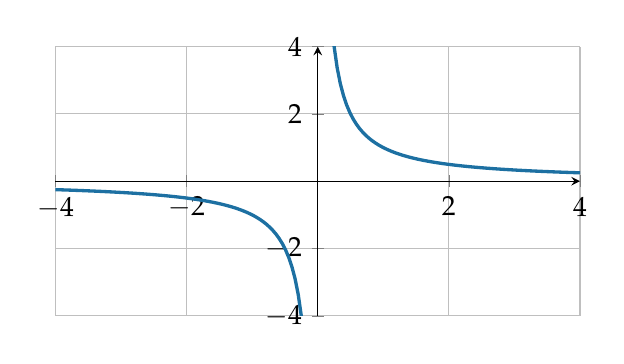
\begin{tikzpicture}\begin{axis}[width=.68\textwidth,height=5cm,axis lines=middle,xmin=-4,xmax=4,ymin=-4,ymax=4,grid=major]\addplot[Blue,very thick,samples=80,domain=-4:-.15]{1/x};\addplot[Blue,very thick,samples=80,domain=.15:4]{1/x};\end{axis}\end{tikzpicture}\end{center}
\end{activite}
\enseignant{Les valeurs sont respectivement $-\frac14,-\frac12,-1,-2,2,1,\frac12,\frac14$. Le domaine exclut $0$ ; la courbe est symétrique par rapport à l'origine. Faire verbaliser la donnée qui déclenche le choix de méthode.}

\begin{traceecrite}La fonction inverse est $f(x)=\dfrac1x$ sur $\R\setminus\{0\}$. Sa courbe est une hyperbole symétrique par rapport à l'origine.\end{traceecrite}

\begin{exemple}
Reprendre les données de l'activité et rédiger la solution dans l'ordre : définition des objets, propriété utilisée, calcul exact ou approché, puis phrase de réponse. La réponse modèle figure dans l'édition enseignant.
\end{exemple}
\enseignant{Les valeurs sont respectivement $-\frac14,-\frac12,-1,-2,2,1,\frac12,\frac14$. Le domaine exclut $0$ ; la courbe est symétrique par rapport à l'origine.}

\begin{exercice}[-- essentiel]
\begin{enumerate}\item Donner le domaine et les asymptotes de $f(x)=5+\dfrac{7}x$.\item Calculer $f'(x)$ et étudier son signe.\item Étudier sur $]0,+\infty[$ la fonction $g(x)=x+\dfrac{25}x$.\end{enumerate}
\end{exercice}
\enseignant{Le domaine est $\R\setminus\{0\}$ ; asymptotes $x=0$ et $y=5$. $f'(x)=-\dfrac{7}{x^2}<0$. Pour $g$, $g'(x)=1-\dfrac{25}{x^2}$ et le minimum est atteint en $x=5$, de valeur $10$.}

\manuelref{Calao, cours p. 88--93 ; exercices p. 94, n° 1 à 5}
\ExoSession{23}

\begin{dm}Reprendre l'exercice d'entraînement 2 avec les données suivantes : remplacer la donnée initiale par $235$ et le taux ou la raison par $7$. Rédiger en quatre lignes : données, formule, calcul, conclusion.\end{dm}
\enseignant{La correction dépend de l'exercice repris. Vérifier surtout la cohérence du modèle, le nombre d'itérations, l'arrondi et la phrase de conclusion.}

\begin{sortie}Sur une demi-feuille : écrire la règle principale de la séance, traiter un exemple très court et indiquer son degré de confiance de 1 à 4. Question(s) essentielle(s) du jour : 1, 2 et 3.\end{sortie}

\ifprof
\begin{methode}
\textbf{Conduite en 1 h :} 7 min d'automatismes ; 10 min de mise en commun et trace ; 28 min d'exercices essentiels ; 5 min de correction ; 3 min de billet de sortie.\\
\textbf{Conduite en 2 h :} ajouter 20 min de recherche de l'activité, 20 min d'institutionnalisation, un second exercice autonome et 10 min de correction comparée.\\
\textbf{Différenciation :} fournir aux élèves fragiles une fiche à quatre cases (données, modèle, calcul, conclusion). Demander aux élèves rapides de produire un contre-exemple, une justification ou une seconde méthode.
\end{methode}
\fi
\sessionheader{24}{17/12/2026}{B : 1 h -- C : 2 h}{Comportement aux bornes et asymptotes}{Fonction inverse}
\begin{objectifs}\begin{itemize}\item Décrire le comportement aux bornes.\item Identifier les asymptotes.\item Lire une représentation.\end{itemize}\end{objectifs}
\begin{automatismes}\begin{enumerate}\item Calculer $5\,\%$ de $120$. \rep{$6$}\item Calculer $\dfrac1{6}$ et $\dfrac1{-6}$. \rep{$\dfrac1{6}$ et $-\dfrac1{6}$}\item Dériver $3x^2-5x+1$. \rep{$6x-5$}\item Résoudre $(x-2)(x+1)=0$. \rep{$x=-1$ ou $x=2$}\item Donner la valeur interdite de $\dfrac{x+1}{x}$. \rep{$x=0$}\end{enumerate}\end{automatismes}
\begin{prerequis}Relire la dernière trace écrite et savoir effectuer les calculs élémentaires mobilisés aujourd'hui. Avant l'activité, faire reformuler les mots-clés : décrire le comportement aux bornes et identifier les asymptotes.\end{prerequis}

\begin{activite}
À l'aide d'un tableau de valeurs près de $0$ et pour de grandes valeurs de $|x|$, décrire $\dfrac1x$. Traduire chaque comportement par une asymptote et par une phrase.
\begin{center}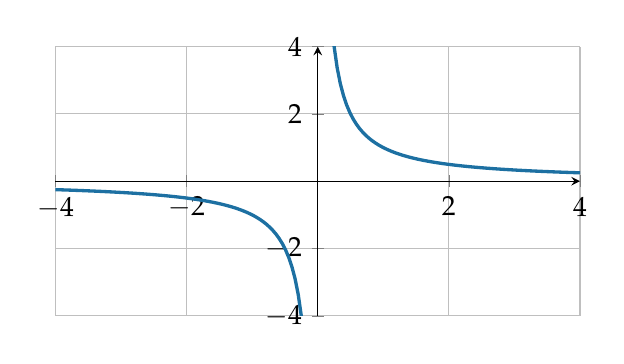
\begin{tikzpicture}\begin{axis}[width=.68\textwidth,height=5cm,axis lines=middle,xmin=-4,xmax=4,ymin=-4,ymax=4,grid=major]\addplot[Blue,very thick,samples=80,domain=-4:-.15]{1/x};\addplot[Blue,very thick,samples=80,domain=.15:4]{1/x};\end{axis}\end{tikzpicture}\end{center}
\end{activite}
\enseignant{Près de $0$, les valeurs deviennent très grandes en valeur absolue : asymptote $x=0$. Quand $|x|$ grandit, $\dfrac1x$ se rapproche de $0$ : asymptote $y=0$. Faire verbaliser la donnée qui déclenche le choix de méthode.}

\begin{traceecrite}Pour $f(x)=\dfrac1x$, $x=0$ est asymptote verticale et $y=0$ asymptote horizontale. Les branches s'en approchent sans les couper.\end{traceecrite}

\begin{exemple}
Reprendre les données de l'activité et rédiger la solution dans l'ordre : définition des objets, propriété utilisée, calcul exact ou approché, puis phrase de réponse. La réponse modèle figure dans l'édition enseignant.
\end{exemple}
\enseignant{Près de $0$, les valeurs deviennent très grandes en valeur absolue : asymptote $x=0$. Quand $|x|$ grandit, $\dfrac1x$ se rapproche de $0$ : asymptote $y=0$.}

\begin{exercice}[-- essentiel]
\begin{enumerate}\item Donner le domaine et les asymptotes de $f(x)=6+\dfrac{8}x$.\item Calculer $f'(x)$ et étudier son signe.\item Étudier sur $]0,+\infty[$ la fonction $g(x)=x+\dfrac{36}x$.\end{enumerate}
\end{exercice}
\enseignant{Le domaine est $\R\setminus\{0\}$ ; asymptotes $x=0$ et $y=6$. $f'(x)=-\dfrac{8}{x^2}<0$. Pour $g$, $g'(x)=1-\dfrac{36}{x^2}$ et le minimum est atteint en $x=6$, de valeur $12$.}

\manuelref{Calao, cours p. 88--93 ; exercices p. 94, n° 4 à 9}
\ExoSession{24}

\begin{dm}Reprendre l'exercice d'entraînement 3 avec les données suivantes : remplacer la donnée initiale par $240$ et le taux ou la raison par $2$. Rédiger en quatre lignes : données, formule, calcul, conclusion.\end{dm}
\enseignant{La correction dépend de l'exercice repris. Vérifier surtout la cohérence du modèle, le nombre d'itérations, l'arrondi et la phrase de conclusion.}

\begin{sortie}Sur une demi-feuille : écrire la règle principale de la séance, traiter un exemple très court et indiquer son degré de confiance de 1 à 4. Question(s) essentielle(s) du jour : 1 et 2.\end{sortie}

\ifprof
\begin{methode}
\textbf{Conduite en 1 h :} 7 min d'automatismes ; 10 min de mise en commun et trace ; 28 min d'exercices essentiels ; 5 min de correction ; 3 min de billet de sortie.\\
\textbf{Conduite en 2 h :} ajouter 20 min de recherche de l'activité, 20 min d'institutionnalisation, un second exercice autonome et 10 min de correction comparée.\\
\textbf{Différenciation :} fournir aux élèves fragiles une fiche à quatre cases (données, modèle, calcul, conclusion). Demander aux élèves rapides de produire un contre-exemple, une justification ou une seconde méthode.
\end{methode}
\fi
\sessionheader{25}{05/01/2027}{B : 2 h -- C : 1 h}{Dérivée et sens de variation}{Fonction inverse}
\begin{objectifs}\begin{itemize}\item Dériver la fonction inverse.\item Justifier les variations.\item Dresser un tableau.\end{itemize}\end{objectifs}
\begin{automatismes}\begin{enumerate}\item Écrire le coefficient multiplicateur d'une hausse de $10\,\%$. \rep{$1+\dfrac{10}{100}=1,10$}\item Dériver $3x^2-5x+1$. \rep{$6x-5$}\item Résoudre $(x-2)(x+1)=0$. \rep{$x=-1$ ou $x=2$}\item Donner la valeur interdite de $\dfrac{x+1}{x}$. \rep{$x=0$}\item Calculer $\dfrac1{7}$ et $\dfrac1{-7}$. \rep{$\dfrac1{7}$ et $-\dfrac1{7}$}\end{enumerate}\end{automatismes}
\begin{prerequis}Relire la dernière trace écrite et savoir effectuer les calculs élémentaires mobilisés aujourd'hui. Avant l'activité, faire reformuler les mots-clés : dériver la fonction inverse et justifier les variations.\end{prerequis}

\begin{activite}
À partir du taux d'accroissement de $f(x)=\dfrac1x$, retrouver $f'(x)=-\dfrac1{x^2}$. Étudier son signe et vérifier la cohérence avec le graphique.

\end{activite}
\enseignant{Le carré $x^2$ est positif pour $x\neq0$, donc la dérivée est strictement négative sur chacun des intervalles du domaine. Faire verbaliser la donnée qui déclenche le choix de méthode.}

\begin{traceecrite}Pour $x\neq0$, $f'(x)=-\dfrac1{x^2}<0$. La fonction inverse décroît sur chacun des intervalles $]-\infty,0[$ et $]0,+\infty[$.\end{traceecrite}

\begin{exemple}
Reprendre les données de l'activité et rédiger la solution dans l'ordre : définition des objets, propriété utilisée, calcul exact ou approché, puis phrase de réponse. La réponse modèle figure dans l'édition enseignant.
\end{exemple}
\enseignant{Le carré $x^2$ est positif pour $x\neq0$, donc la dérivée est strictement négative sur chacun des intervalles du domaine.}

\begin{exercice}[-- essentiel]
\begin{enumerate}\item Donner le domaine et les asymptotes de $f(x)=2+\dfrac{4}x$.\item Calculer $f'(x)$ et étudier son signe.\item Étudier sur $]0,+\infty[$ la fonction $g(x)=x+\dfrac{4}x$.\end{enumerate}
\end{exercice}
\enseignant{Le domaine est $\R\setminus\{0\}$ ; asymptotes $x=0$ et $y=2$. $f'(x)=-\dfrac{4}{x^2}<0$. Pour $g$, $g'(x)=1-\dfrac{4}{x^2}$ et le minimum est atteint en $x=2$, de valeur $4$.}

\manuelref{Calao, cours p. 89--93 ; exercices p. 94, n° 1 à 3, puis p. 96, n° 10 à 13}
\ExoSession{25}

\begin{dm}Reprendre l'exercice d'entraînement 2 avec les données suivantes : remplacer la donnée initiale par $245$ et le taux ou la raison par $3$. Rédiger en quatre lignes : données, formule, calcul, conclusion.\end{dm}
\enseignant{La correction dépend de l'exercice repris. Vérifier surtout la cohérence du modèle, le nombre d'itérations, l'arrondi et la phrase de conclusion.}

\begin{sortie}Sur une demi-feuille : écrire la règle principale de la séance, traiter un exemple très court et indiquer son degré de confiance de 1 à 4. Question(s) essentielle(s) du jour : 1, 2 et 3.\end{sortie}

\ifprof
\begin{methode}
\textbf{Conduite en 1 h :} 7 min d'automatismes ; 10 min de mise en commun et trace ; 28 min d'exercices essentiels ; 5 min de correction ; 3 min de billet de sortie.\\
\textbf{Conduite en 2 h :} ajouter 20 min de recherche de l'activité, 20 min d'institutionnalisation, un second exercice autonome et 10 min de correction comparée.\\
\textbf{Différenciation :} fournir aux élèves fragiles une fiche à quatre cases (données, modèle, calcul, conclusion). Demander aux élèves rapides de produire un contre-exemple, une justification ou une seconde méthode.
\end{methode}
\fi
\sessionheader{26}{07/01/2027}{B : 1 h -- C : 2 h}{Combinaisons avec des fonctions polynomiales}{Fonction inverse}
\begin{objectifs}\begin{itemize}\item Dériver une combinaison.\item Réduire une expression.\item Organiser une étude.\end{itemize}\end{objectifs}
\begin{automatismes}\begin{enumerate}\item Réduire $3x+8-x+2$. \rep{$2x+10$}\item Résoudre $(x-2)(x+1)=0$. \rep{$x=-1$ ou $x=2$}\item Donner la valeur interdite de $\dfrac{x+1}{x}$. \rep{$x=0$}\item Calculer $\dfrac1{8}$ et $\dfrac1{-8}$. \rep{$\dfrac1{8}$ et $-\dfrac1{8}$}\item Dériver $3x^2-5x+1$. \rep{$6x-5$}\end{enumerate}\end{automatismes}
\begin{prerequis}Relire la dernière trace écrite et savoir effectuer les calculs élémentaires mobilisés aujourd'hui. Avant l'activité, faire reformuler les mots-clés : dériver une combinaison et réduire une expression.\end{prerequis}

\begin{activite}
Une entreprise produit $x>0$ centaines d'objets et son coût moyen est $C(x)=2x+30+\dfrac{200}{x}$. Calculer $C'(x)$, factoriser son numérateur et chercher le niveau de production minimisant le coût moyen.

\end{activite}
\enseignant{$C'(x)=2-\dfrac{200}{x^2}=\dfrac{2(x-10)(x+10)}{x^2}$. Le minimum est atteint pour $x=10$, soit $1\,000$ objets. Faire verbaliser la donnée qui déclenche le choix de méthode.}

\begin{traceecrite}Pour étudier $P(x)+\dfrac{k}{x}$, déterminer le domaine, calculer la dérivée, réduire au même dénominateur, étudier son signe puis dresser les variations.\end{traceecrite}

\begin{exemple}
Reprendre les données de l'activité et rédiger la solution dans l'ordre : définition des objets, propriété utilisée, calcul exact ou approché, puis phrase de réponse. La réponse modèle figure dans l'édition enseignant.
\end{exemple}
\enseignant{$C'(x)=2-\dfrac{200}{x^2}=\dfrac{2(x-10)(x+10)}{x^2}$. Le minimum est atteint pour $x=10$, soit $1\,000$ objets.}

\begin{exercice}[-- essentiel]
\begin{enumerate}\item Donner le domaine et les asymptotes de $f(x)=3+\dfrac{5}x$.\item Calculer $f'(x)$ et étudier son signe.\item Étudier sur $]0,+\infty[$ la fonction $g(x)=x+\dfrac{9}x$.\end{enumerate}
\end{exercice}
\enseignant{Le domaine est $\R\setminus\{0\}$ ; asymptotes $x=0$ et $y=3$. $f'(x)=-\dfrac{5}{x^2}<0$. Pour $g$, $g'(x)=1-\dfrac{9}{x^2}$ et le minimum est atteint en $x=3$, de valeur $6$.}

\manuelref{Calao, p. 96, n° 14 à 21}
\ExoSession{26}

\begin{dm}Reprendre l'exercice d'entraînement 3 avec les données suivantes : remplacer la donnée initiale par $250$ et le taux ou la raison par $4$. Rédiger en quatre lignes : données, formule, calcul, conclusion.\end{dm}
\enseignant{La correction dépend de l'exercice repris. Vérifier surtout la cohérence du modèle, le nombre d'itérations, l'arrondi et la phrase de conclusion.}

\begin{sortie}Sur une demi-feuille : écrire la règle principale de la séance, traiter un exemple très court et indiquer son degré de confiance de 1 à 4. Question(s) essentielle(s) du jour : 1 et 2.\end{sortie}

\ifprof
\begin{methode}
\textbf{Conduite en 1 h :} 7 min d'automatismes ; 10 min de mise en commun et trace ; 28 min d'exercices essentiels ; 5 min de correction ; 3 min de billet de sortie.\\
\textbf{Conduite en 2 h :} ajouter 20 min de recherche de l'activité, 20 min d'institutionnalisation, un second exercice autonome et 10 min de correction comparée.\\
\textbf{Différenciation :} fournir aux élèves fragiles une fiche à quatre cases (données, modèle, calcul, conclusion). Demander aux élèves rapides de produire un contre-exemple, une justification ou une seconde méthode.
\end{methode}
\fi
\sessionheader{27}{12/01/2027}{B : 2 h -- C : 1 h}{Signe et factorisation}{Fonction inverse}
\begin{objectifs}\begin{itemize}\item Factoriser.\item Construire un tableau de signes.\item Respecter les valeurs interdites.\end{itemize}\end{objectifs}
\begin{automatismes}\begin{enumerate}\item Calculer $20\,\%$ de $180$. \rep{$36$}\item Donner la valeur interdite de $\dfrac{x+1}{x}$. \rep{$x=0$}\item Calculer $\dfrac1{9}$ et $\dfrac1{-9}$. \rep{$\dfrac1{9}$ et $-\dfrac1{9}$}\item Dériver $3x^2-5x+1$. \rep{$6x-5$}\item Résoudre $(x-2)(x+1)=0$. \rep{$x=-1$ ou $x=2$}\end{enumerate}\end{automatismes}
\begin{prerequis}Relire la dernière trace écrite et savoir effectuer les calculs élémentaires mobilisés aujourd'hui. Avant l'activité, faire reformuler les mots-clés : factoriser et construire un tableau de signes.\end{prerequis}

\begin{activite}
Étudier le signe de $\dfrac{(x-2)(x+3)}x$. Construire le tableau avec les trois valeurs critiques, distinguer zéro et valeur interdite, puis résoudre l'inéquation $\dfrac{(x-2)(x+3)}x\geq0$.

\end{activite}
\enseignant{Les valeurs critiques sont $-3,0,2$. La solution est $[-3,0[\cup[2,+\infty[$. Faire verbaliser la donnée qui déclenche le choix de méthode.}

\begin{traceecrite}Dans un quotient, le signe dépend du numérateur et du dénominateur. Les valeurs interdites sont exclues du tableau, même si un facteur se simplifie formellement.\end{traceecrite}

\begin{exemple}
Reprendre les données de l'activité et rédiger la solution dans l'ordre : définition des objets, propriété utilisée, calcul exact ou approché, puis phrase de réponse. La réponse modèle figure dans l'édition enseignant.
\end{exemple}
\enseignant{Les valeurs critiques sont $-3,0,2$. La solution est $[-3,0[\cup[2,+\infty[$.}

\begin{exercice}[-- essentiel]
\begin{enumerate}\item Donner le domaine et les asymptotes de $f(x)=4+\dfrac{6}x$.\item Calculer $f'(x)$ et étudier son signe.\item Étudier sur $]0,+\infty[$ la fonction $g(x)=x+\dfrac{16}x$.\end{enumerate}
\end{exercice}
\enseignant{Le domaine est $\R\setminus\{0\}$ ; asymptotes $x=0$ et $y=4$. $f'(x)=-\dfrac{6}{x^2}<0$. Pour $g$, $g'(x)=1-\dfrac{16}{x^2}$ et le minimum est atteint en $x=4$, de valeur $8$.}

\manuelref{Calao, p. 96 à 101}
\ExoSession{27}

\begin{dm}Reprendre l'exercice d'entraînement 2 avec les données suivantes : remplacer la donnée initiale par $255$ et le taux ou la raison par $5$. Rédiger en quatre lignes : données, formule, calcul, conclusion.\end{dm}
\enseignant{La correction dépend de l'exercice repris. Vérifier surtout la cohérence du modèle, le nombre d'itérations, l'arrondi et la phrase de conclusion.}

\begin{sortie}Sur une demi-feuille : écrire la règle principale de la séance, traiter un exemple très court et indiquer son degré de confiance de 1 à 4. Question(s) essentielle(s) du jour : 1, 2 et 3.\end{sortie}

\ifprof
\begin{methode}
\textbf{Conduite en 1 h :} 7 min d'automatismes ; 10 min de mise en commun et trace ; 28 min d'exercices essentiels ; 5 min de correction ; 3 min de billet de sortie.\\
\textbf{Conduite en 2 h :} ajouter 20 min de recherche de l'activité, 20 min d'institutionnalisation, un second exercice autonome et 10 min de correction comparée.\\
\textbf{Différenciation :} fournir aux élèves fragiles une fiche à quatre cases (données, modèle, calcul, conclusion). Demander aux élèves rapides de produire un contre-exemple, une justification ou une seconde méthode.
\end{methode}
\fi
\sessionheader{28}{14/01/2027}{B : 1 h -- C : 2 h}{Dérivées de polynômes de degré au plus 3}{Fonction inverse}
\begin{objectifs}\begin{itemize}\item Dériver un polynôme.\item Étudier une dérivée.\item Déduire des variations.\end{itemize}\end{objectifs}
\begin{automatismes}\begin{enumerate}\item Écrire le coefficient multiplicateur d'une hausse de $25\,\%$. \rep{$1+\dfrac{25}{100}=1,25$}\item Calculer $\dfrac1{3}$ et $\dfrac1{-3}$. \rep{$\dfrac1{3}$ et $-\dfrac1{3}$}\item Dériver $3x^2-5x+1$. \rep{$6x-5$}\item Résoudre $(x-2)(x+1)=0$. \rep{$x=-1$ ou $x=2$}\item Donner la valeur interdite de $\dfrac{x+1}{x}$. \rep{$x=0$}\end{enumerate}\end{automatismes}
\begin{prerequis}Relire la dernière trace écrite et savoir effectuer les calculs élémentaires mobilisés aujourd'hui. Avant l'activité, faire reformuler les mots-clés : dériver un polynôme et étudier une dérivée.\end{prerequis}

\begin{activite}
Pour $f(x)=2x^3-3x^2-12x+5$, calculer $f'(x)$, factoriser, étudier son signe et en déduire les variations de $f$.

\end{activite}
\enseignant{$f'(x)=6x^2-6x-12=6(x-2)(x+1)$. La fonction croît sur $]-\infty,-1]$, décroît sur $[-1,2]$, puis croît. Faire verbaliser la donnée qui déclenche le choix de méthode.}

\begin{traceecrite}$(ax^3+bx^2+cx+d)'=3ax^2+2bx+c$. Le signe de la dérivée donne le sens de variation de la fonction.\end{traceecrite}

\begin{exemple}
Reprendre les données de l'activité et rédiger la solution dans l'ordre : définition des objets, propriété utilisée, calcul exact ou approché, puis phrase de réponse. La réponse modèle figure dans l'édition enseignant.
\end{exemple}
\enseignant{$f'(x)=6x^2-6x-12=6(x-2)(x+1)$. La fonction croît sur $]-\infty,-1]$, décroît sur $[-1,2]$, puis croît.}

\begin{exercice}[-- essentiel]
\begin{enumerate}\item Donner le domaine et les asymptotes de $f(x)=5+\dfrac{7}x$.\item Calculer $f'(x)$ et étudier son signe.\item Étudier sur $]0,+\infty[$ la fonction $g(x)=x+\dfrac{25}x$.\end{enumerate}
\end{exercice}
\enseignant{Le domaine est $\R\setminus\{0\}$ ; asymptotes $x=0$ et $y=5$. $f'(x)=-\dfrac{7}{x^2}<0$. Pour $g$, $g'(x)=1-\dfrac{25}{x^2}$ et le minimum est atteint en $x=5$, de valeur $10$.}

\manuelref{Calao, p. 94 à 96}
\ExoSession{28}

\begin{dm}Reprendre l'exercice d'entraînement 3 avec les données suivantes : remplacer la donnée initiale par $260$ et le taux ou la raison par $6$. Rédiger en quatre lignes : données, formule, calcul, conclusion.\end{dm}
\enseignant{La correction dépend de l'exercice repris. Vérifier surtout la cohérence du modèle, le nombre d'itérations, l'arrondi et la phrase de conclusion.}

\begin{sortie}Sur une demi-feuille : écrire la règle principale de la séance, traiter un exemple très court et indiquer son degré de confiance de 1 à 4. Question(s) essentielle(s) du jour : 1 et 2.\end{sortie}

\ifprof
\begin{methode}
\textbf{Conduite en 1 h :} 7 min d'automatismes ; 10 min de mise en commun et trace ; 28 min d'exercices essentiels ; 5 min de correction ; 3 min de billet de sortie.\\
\textbf{Conduite en 2 h :} ajouter 20 min de recherche de l'activité, 20 min d'institutionnalisation, un second exercice autonome et 10 min de correction comparée.\\
\textbf{Différenciation :} fournir aux élèves fragiles une fiche à quatre cases (données, modèle, calcul, conclusion). Demander aux élèves rapides de produire un contre-exemple, une justification ou une seconde méthode.
\end{methode}
\fi
\sessionheader{29}{19/01/2027}{B : 2 h -- C : 1 h}{Étude complète et représentation}{Fonction inverse}
\begin{objectifs}\begin{itemize}\item Mener une étude complète.\item Tracer une courbe cohérente.\item Interpréter un extremum.\end{itemize}\end{objectifs}
\begin{automatismes}\begin{enumerate}\item Réduire $3x+4-x+2$. \rep{$2x+6$}\item Dériver $3x^2-5x+1$. \rep{$6x-5$}\item Résoudre $(x-2)(x+1)=0$. \rep{$x=-1$ ou $x=2$}\item Donner la valeur interdite de $\dfrac{x+1}{x}$. \rep{$x=0$}\item Calculer $\dfrac1{4}$ et $\dfrac1{-4}$. \rep{$\dfrac1{4}$ et $-\dfrac1{4}$}\end{enumerate}\end{automatismes}
\begin{prerequis}Relire la dernière trace écrite et savoir effectuer les calculs élémentaires mobilisés aujourd'hui. Avant l'activité, faire reformuler les mots-clés : mener une étude complète et tracer une courbe cohérente.\end{prerequis}

\begin{activite}
Étudier complètement $g(x)=x+\dfrac9x$ sur $]0,+\infty[$ : domaine, dérivée, signe, variations, minimum, comportement aux bornes et esquisse.
\begin{center}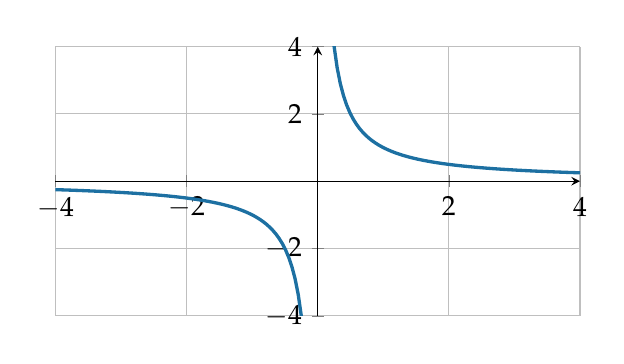
\begin{tikzpicture}\begin{axis}[width=.68\textwidth,height=5cm,axis lines=middle,xmin=-4,xmax=4,ymin=-4,ymax=4,grid=major]\addplot[Blue,very thick,samples=80,domain=-4:-.15]{1/x};\addplot[Blue,very thick,samples=80,domain=.15:4]{1/x};\end{axis}\end{tikzpicture}\end{center}
\end{activite}
\enseignant{$g'(x)=\dfrac{(x-3)(x+3)}{x^2}$ ; minimum $g(3)=6$ ; $g(x)$ tend vers $+\infty$ en $0^+$ et en $+\infty$. Faire verbaliser la donnée qui déclenche le choix de méthode.}

\begin{traceecrite}Une étude complète comporte : domaine, dérivée, signe, variations, limites ou comportement aux bornes, points remarquables et graphique cohérent.\end{traceecrite}

\begin{exemple}
Reprendre les données de l'activité et rédiger la solution dans l'ordre : définition des objets, propriété utilisée, calcul exact ou approché, puis phrase de réponse. La réponse modèle figure dans l'édition enseignant.
\end{exemple}
\enseignant{$g'(x)=\dfrac{(x-3)(x+3)}{x^2}$ ; minimum $g(3)=6$ ; $g(x)$ tend vers $+\infty$ en $0^+$ et en $+\infty$.}

\begin{exercice}[-- essentiel]
\begin{enumerate}\item Donner le domaine et les asymptotes de $f(x)=6+\dfrac{8}x$.\item Calculer $f'(x)$ et étudier son signe.\item Étudier sur $]0,+\infty[$ la fonction $g(x)=x+\dfrac{36}x$.\end{enumerate}
\end{exercice}
\enseignant{Le domaine est $\R\setminus\{0\}$ ; asymptotes $x=0$ et $y=6$. $f'(x)=-\dfrac{8}{x^2}<0$. Pour $g$, $g'(x)=1-\dfrac{36}{x^2}$ et le minimum est atteint en $x=6$, de valeur $12$.}

\manuelref{Calao, p. 98 à 103}
\ExoSession{29}

\begin{dm}Reprendre l'exercice d'entraînement 2 avec les données suivantes : remplacer la donnée initiale par $265$ et le taux ou la raison par $7$. Rédiger en quatre lignes : données, formule, calcul, conclusion.\end{dm}
\enseignant{La correction dépend de l'exercice repris. Vérifier surtout la cohérence du modèle, le nombre d'itérations, l'arrondi et la phrase de conclusion.}

\begin{sortie}Sur une demi-feuille : écrire la règle principale de la séance, traiter un exemple très court et indiquer son degré de confiance de 1 à 4. Question(s) essentielle(s) du jour : 1, 2 et 3.\end{sortie}

\ifprof
\begin{methode}
\textbf{Conduite en 1 h :} 7 min d'automatismes ; 10 min de mise en commun et trace ; 28 min d'exercices essentiels ; 5 min de correction ; 3 min de billet de sortie.\\
\textbf{Conduite en 2 h :} ajouter 20 min de recherche de l'activité, 20 min d'institutionnalisation, un second exercice autonome et 10 min de correction comparée.\\
\textbf{Différenciation :} fournir aux élèves fragiles une fiche à quatre cases (données, modèle, calcul, conclusion). Demander aux élèves rapides de produire un contre-exemple, une justification ou une seconde méthode.
\end{methode}
\fi
\sessionheader{30}{21/01/2027}{B : 1 h -- C : 2 h}{Bilan et évaluation}{Fonction inverse}
\begin{objectifs}\begin{itemize}\item Mobiliser domaine, dérivée et signe.\item Rédiger une étude.\item Corriger méthodiquement.\end{itemize}\end{objectifs}
\begin{automatismes}\begin{enumerate}\item Calculer $5\,\%$ de $100$. \rep{$5$}\item Résoudre $(x-2)(x+1)=0$. \rep{$x=-1$ ou $x=2$}\item Donner la valeur interdite de $\dfrac{x+1}{x}$. \rep{$x=0$}\item Calculer $\dfrac1{5}$ et $\dfrac1{-5}$. \rep{$\dfrac1{5}$ et $-\dfrac1{5}$}\item Dériver $3x^2-5x+1$. \rep{$6x-5$}\end{enumerate}\end{automatismes}
\begin{prerequis}Relire la dernière trace écrite et savoir effectuer les calculs élémentaires mobilisés aujourd'hui. Avant l'activité, faire reformuler les mots-clés : mobiliser domaine, dérivée et signe et rédiger une étude.\end{prerequis}

\begin{activite}
Corriger une étude volontairement erronée de $h(x)=x+\dfrac4x$ : domaine annoncé $\R$, dérivée $1+\dfrac4{x^2}$, tableau sans rupture en $0$. Réécrire une solution complète.

\end{activite}
\enseignant{Le domaine est $\R\setminus\{0\}$ et $h'(x)=1-\dfrac4{x^2}$. Le tableau est séparé en $0$ et tient compte de $-2$ et $2$. Faire verbaliser la donnée qui déclenche le choix de méthode.}

\begin{traceecrite}Contrôler séparément les quatre objets : domaine, expression de la dérivée, signe de la dérivée, variations. Une erreur à une étape ne doit pas masquer les suivantes.\end{traceecrite}

\begin{exemple}
Reprendre les données de l'activité et rédiger la solution dans l'ordre : définition des objets, propriété utilisée, calcul exact ou approché, puis phrase de réponse. La réponse modèle figure dans l'édition enseignant.
\end{exemple}
\enseignant{Le domaine est $\R\setminus\{0\}$ et $h'(x)=1-\dfrac4{x^2}$. Le tableau est séparé en $0$ et tient compte de $-2$ et $2$.}

\begin{exercice}[-- essentiel]
\begin{enumerate}\item Donner le domaine et les asymptotes de $f(x)=2+\dfrac{4}x$.\item Calculer $f'(x)$ et étudier son signe.\item Étudier sur $]0,+\infty[$ la fonction $g(x)=x+\dfrac{4}x$.\end{enumerate}
\end{exercice}
\enseignant{Le domaine est $\R\setminus\{0\}$ ; asymptotes $x=0$ et $y=2$. $f'(x)=-\dfrac{4}{x^2}<0$. Pour $g$, $g'(x)=1-\dfrac{4}{x^2}$ et le minimum est atteint en $x=2$, de valeur $4$.}

\manuelref{Calao, p. 100 à 103}
\ExoSession{30}

\begin{dm}Reprendre l'exercice d'entraînement 3 avec les données suivantes : remplacer la donnée initiale par $270$ et le taux ou la raison par $2$. Rédiger en quatre lignes : données, formule, calcul, conclusion.\end{dm}
\enseignant{La correction dépend de l'exercice repris. Vérifier surtout la cohérence du modèle, le nombre d'itérations, l'arrondi et la phrase de conclusion.}

\begin{sortie}Sur une demi-feuille : écrire la règle principale de la séance, traiter un exemple très court et indiquer son degré de confiance de 1 à 4. Question(s) essentielle(s) du jour : 1 et 2.\end{sortie}

\ifprof
\begin{methode}
\textbf{Conduite en 1 h :} 7 min d'automatismes ; 10 min de mise en commun et trace ; 28 min d'exercices essentiels ; 5 min de correction ; 3 min de billet de sortie.\\
\textbf{Conduite en 2 h :} ajouter 20 min de recherche de l'activité, 20 min d'institutionnalisation, un second exercice autonome et 10 min de correction comparée.\\
\textbf{Différenciation :} fournir aux élèves fragiles une fiche à quatre cases (données, modèle, calcul, conclusion). Demander aux élèves rapides de produire un contre-exemple, une justification ou une seconde méthode.
\end{methode}
\fi


\chapter{Statistiques à deux variables quantitatives}
\competences{représenter, choisir un ajustement, interpoler, extrapoler avec prudence, communiquer}
\section{Cours de référence}
Une série statistique à deux variables est constituée de couples $(x_i,y_i)$. Le nuage de points permet d'observer une tendance, une dispersion et d'éventuelles valeurs atypiques.

\begin{center}
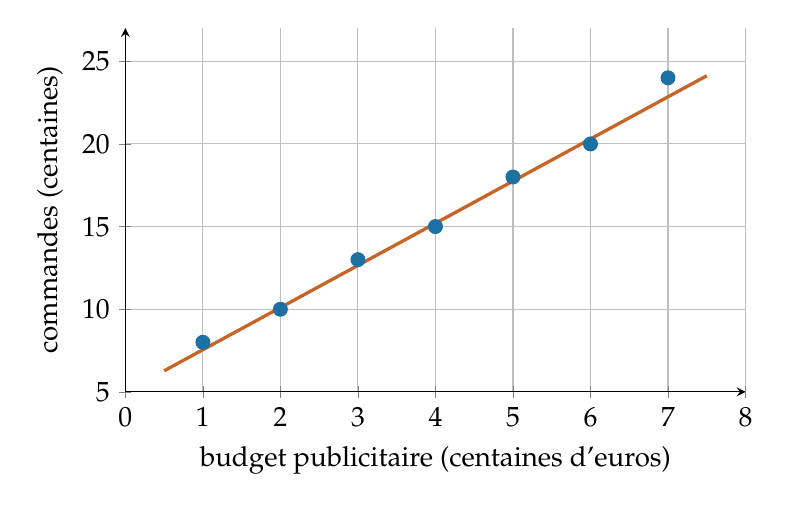
\begin{tikzpicture}
\begin{axis}[width=.78\textwidth,height=6.2cm,axis lines=left,xmin=0,xmax=8,ymin=5,ymax=27,grid=major,xlabel={budget publicitaire (centaines d'euros)},ylabel={commandes (centaines)}]
\addplot[only marks,mark=*,Blue,mark size=2.5pt] coordinates {(1,8)(2,10)(3,13)(4,15)(5,18)(6,20)(7,24)};
\addplot[Orange,very thick,domain=.5:7.5]{2.55*x+5};
\end{axis}
\end{tikzpicture}
\end{center}

\begin{retenir}
Une droite d'ajustement $y=ax+b$ fournit des estimations, pas des égalités exactes. Le coefficient $a$ décrit la variation moyenne estimée de $y$ quand $x$ augmente d'une unité. Une interpolation reste dans l'intervalle des valeurs observées ; une extrapolation sort de cet intervalle et doit être présentée avec prudence.
\end{retenir}

Le point moyen $G(\bar x,\bar y)$ a pour coordonnées $\bar x=\dfrac{x_1+\cdots+x_n}{n}$ et $\bar y=\dfrac{y_1+\cdots+y_n}{n}$. Une droite de régression obtenue à la calculatrice passe par $G$, à l'arrondi près.

\begin{methode}
Pour exploiter $y=ax+b$ : 1) remplacer $x$ par la valeur demandée pour estimer $y$ ; 2) résoudre $ax+b=y_0$ pour estimer $x$ ; 3) arrondir selon le contexte ; 4) préciser interpolation ou extrapolation ; 5) rappeler que le résultat dépend du modèle.
\end{methode}

Un changement de variable, par exemple $z=\log(y)$ ou $z=\dfrac1y$, peut rendre un nuage approximativement aligné. On ajuste alors $(x,z)$, puis on revient à la variable $y$.

\sessionheader{31}{26/01/2027}{B : 2 h -- C : 1 h}{Nuage de points}{Statistiques à deux variables}
\begin{objectifs}\begin{itemize}\item Construire un nuage.\item Choisir les échelles.\item Identifier les variables.\end{itemize}\end{objectifs}
\begin{automatismes}\begin{enumerate}\item Écrire le coefficient multiplicateur d'une hausse de $10\,\%$. \rep{$1+\dfrac{10}{100}=1,10$}\item Résoudre $3x+4=25$. \rep{$x=7$}\item Calculer la moyenne de $6$, $8$ et $10$. \rep{$8$}\item Donner la pente entre $(1,3)$ et $(4,9)$. \rep{$\dfrac{9-3}{4-1}=2$}\item Avec $y=2x+5$, calculer $y$ pour $x=7$. \rep{$19$}\end{enumerate}\end{automatismes}
\begin{prerequis}Relire la dernière trace écrite et savoir effectuer les calculs élémentaires mobilisés aujourd'hui. Avant l'activité, faire reformuler les mots-clés : construire un nuage et choisir les échelles.\end{prerequis}

\begin{activite}
Le tableau $(x_i,y_i)$ donne les dépenses publicitaires et les ventes de six mois : $(1,12),(2,15),(3,17),(4,22),(5,24),(6,28)$. Choisir des échelles, tracer le nuage et placer le point moyen.
\begin{center}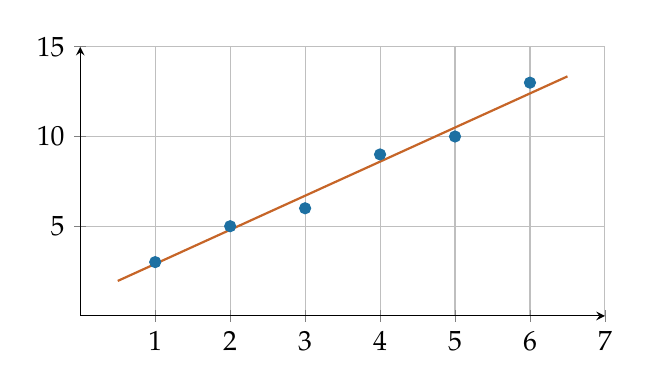
\begin{tikzpicture}\begin{axis}[width=.68\textwidth,height=5cm,axis lines=middle,xmin=0,xmax=7,ymin=0,ymax=15,grid=major]\addplot[only marks,Blue,mark=*] coordinates {(1,3)(2,5)(3,6)(4,9)(5,10)(6,13)};\addplot[Orange,thick,domain=.5:6.5]{1.9*x+1};\end{axis}\end{tikzpicture}\end{center}
\end{activite}
\enseignant{$\bar x=3{,}5$ et $\bar y=19{,}67$ environ. Le nuage présente une tendance croissante approximativement affine. Faire verbaliser la donnée qui déclenche le choix de méthode.}

\begin{traceecrite}Un nuage de points représente les couples $(x_i,y_i)$. Les axes, unités et échelles doivent être indiqués ; chaque couple donne un seul point.\end{traceecrite}

\begin{exemple}
Reprendre les données de l'activité et rédiger la solution dans l'ordre : définition des objets, propriété utilisée, calcul exact ou approché, puis phrase de réponse. La réponse modèle figure dans l'édition enseignant.
\end{exemple}
\enseignant{$\bar x=3{,}5$ et $\bar y=19{,}67$ environ. Le nuage présente une tendance croissante approximativement affine.}

\begin{exercice}[-- essentiel]
\begin{enumerate}\item Pour $y=3x+13$, estimer $y$ lorsque $x=8$.\item Résoudre $3x+13=50$.\item Le modèle a été établi sur $[2,12]$ : qualifier les estimations pour $x=8$ et $x=30$.\end{enumerate}
\end{exercice}
\enseignant{Pour $x=8$, $y=37$. L'équation donne $x=\dfrac{37}{3}$. $x=8$ donne une interpolation ; $x=30$ une extrapolation.}

\manuelref{Calao, cours p. 110--113 ; exercices p. 114, n° 1 à 6}
\CalaoSession{31}

\begin{dm}Reprendre l'exercice d'entraînement 2 avec les données suivantes : remplacer la donnée initiale par $275$ et le taux ou la raison par $3$. Rédiger en quatre lignes : données, formule, calcul, conclusion.\end{dm}
\enseignant{La correction dépend de l'exercice repris. Vérifier surtout la cohérence du modèle, le nombre d'itérations, l'arrondi et la phrase de conclusion.}

\begin{sortie}Sur une demi-feuille : écrire la règle principale de la séance, traiter un exemple très court et indiquer son degré de confiance de 1 à 4. Question(s) essentielle(s) du jour : 1, 2 et 3.\end{sortie}

\ifprof
\begin{methode}
\textbf{Conduite en 1 h :} 7 min d'automatismes ; 10 min de mise en commun et trace ; 28 min d'exercices essentiels ; 5 min de correction ; 3 min de billet de sortie.\\
\textbf{Conduite en 2 h :} ajouter 20 min de recherche de l'activité, 20 min d'institutionnalisation, un second exercice autonome et 10 min de correction comparée.\\
\textbf{Différenciation :} fournir aux élèves fragiles une fiche à quatre cases (données, modèle, calcul, conclusion). Demander aux élèves rapides de produire un contre-exemple, une justification ou une seconde méthode.
\end{methode}
\fi
\sessionheader{32}{28/01/2027}{B : 1 h -- C : 2 h}{Lecture et interprétation du nuage}{Statistiques à deux variables}
\begin{objectifs}\begin{itemize}\item Décrire une tendance.\item Repérer dispersion et atypiques.\item Éviter causalité abusive.\end{itemize}\end{objectifs}
\begin{automatismes}\begin{enumerate}\item Réduire $3x+7-x+2$. \rep{$2x+9$}\item Calculer la moyenne de $7$, $9$ et $11$. \rep{$9$}\item Donner la pente entre $(1,3)$ et $(4,9)$. \rep{$\dfrac{9-3}{4-1}=2$}\item Avec $y=2x+5$, calculer $y$ pour $x=7$. \rep{$19$}\item Résoudre $3x+4=25$. \rep{$x=7$}\end{enumerate}\end{automatismes}
\begin{prerequis}Relire la dernière trace écrite et savoir effectuer les calculs élémentaires mobilisés aujourd'hui. Avant l'activité, faire reformuler les mots-clés : décrire une tendance et repérer dispersion et atypiques.\end{prerequis}

\begin{activite}
Comparer trois nuages : tendance croissante serrée, tendance décroissante dispersée, absence de tendance. Rédiger pour chacun deux phrases sans employer le mot « cause ».

\end{activite}
\enseignant{La description porte sur direction, forme, dispersion et atypiques. Un nuage ne permet pas à lui seul d'établir une causalité. Faire verbaliser la donnée qui déclenche le choix de méthode.}

\begin{traceecrite}Décrire un nuage consiste à commenter la direction, la forme, la dispersion et les valeurs atypiques, sans affirmer une causalité non établie.\end{traceecrite}

\begin{exemple}
Reprendre les données de l'activité et rédiger la solution dans l'ordre : définition des objets, propriété utilisée, calcul exact ou approché, puis phrase de réponse. La réponse modèle figure dans l'édition enseignant.
\end{exemple}
\enseignant{La description porte sur direction, forme, dispersion et atypiques. Un nuage ne permet pas à lui seul d'établir une causalité.}

\begin{exercice}[-- essentiel]
\begin{enumerate}\item Pour $y=4x+14$, estimer $y$ lorsque $x=8$.\item Résoudre $4x+14=50$.\item Le modèle a été établi sur $[2,12]$ : qualifier les estimations pour $x=8$ et $x=30$.\end{enumerate}
\end{exercice}
\enseignant{Pour $x=8$, $y=46$. L'équation donne $x=\dfrac{36}{4}$. $x=8$ donne une interpolation ; $x=30$ une extrapolation.}

\manuelref{Calao, p. 116, n° 11 à 15}
\CalaoSession{32}

\begin{dm}Reprendre l'exercice d'entraînement 3 avec les données suivantes : remplacer la donnée initiale par $280$ et le taux ou la raison par $4$. Rédiger en quatre lignes : données, formule, calcul, conclusion.\end{dm}
\enseignant{La correction dépend de l'exercice repris. Vérifier surtout la cohérence du modèle, le nombre d'itérations, l'arrondi et la phrase de conclusion.}

\begin{sortie}Sur une demi-feuille : écrire la règle principale de la séance, traiter un exemple très court et indiquer son degré de confiance de 1 à 4. Question(s) essentielle(s) du jour : 1 et 2.\end{sortie}

\ifprof
\begin{methode}
\textbf{Conduite en 1 h :} 7 min d'automatismes ; 10 min de mise en commun et trace ; 28 min d'exercices essentiels ; 5 min de correction ; 3 min de billet de sortie.\\
\textbf{Conduite en 2 h :} ajouter 20 min de recherche de l'activité, 20 min d'institutionnalisation, un second exercice autonome et 10 min de correction comparée.\\
\textbf{Différenciation :} fournir aux élèves fragiles une fiche à quatre cases (données, modèle, calcul, conclusion). Demander aux élèves rapides de produire un contre-exemple, une justification ou une seconde méthode.
\end{methode}
\fi
\sessionheader{33}{02/02/2027}{B : 2 h -- C : 1 h}{Ajustement affine}{Statistiques à deux variables}
\begin{objectifs}\begin{itemize}\item Obtenir un ajustement affine.\item Interpréter $a$ et $b$.\item Vérifier avec le point moyen.\end{itemize}\end{objectifs}
\begin{automatismes}\begin{enumerate}\item Calculer $20\,\%$ de $160$. \rep{$32$}\item Donner la pente entre $(1,3)$ et $(4,9)$. \rep{$\dfrac{9-3}{4-1}=2$}\item Avec $y=2x+5$, calculer $y$ pour $x=7$. \rep{$19$}\item Résoudre $3x+4=25$. \rep{$x=7$}\item Calculer la moyenne de $8$, $10$ et $12$. \rep{$10$}\end{enumerate}\end{automatismes}
\begin{prerequis}Relire la dernière trace écrite et savoir effectuer les calculs élémentaires mobilisés aujourd'hui. Avant l'activité, faire reformuler les mots-clés : obtenir un ajustement affine et interpréter $a$ et $b$.\end{prerequis}

\begin{activite}
Avec les données de la séance 31, obtenir la régression affine à la calculatrice. Interpréter la pente et vérifier que le point moyen appartient approximativement à la droite.
\begin{center}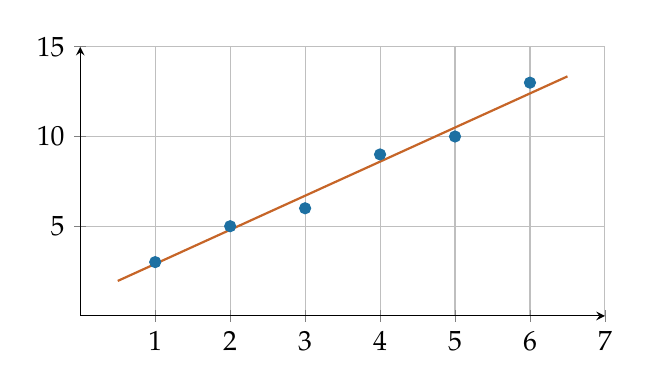
\begin{tikzpicture}\begin{axis}[width=.68\textwidth,height=5cm,axis lines=middle,xmin=0,xmax=7,ymin=0,ymax=15,grid=major]\addplot[only marks,Blue,mark=*] coordinates {(1,3)(2,5)(3,6)(4,9)(5,10)(6,13)};\addplot[Orange,thick,domain=.5:6.5]{1.9*x+1};\end{axis}\end{tikzpicture}\end{center}
\end{activite}
\enseignant{Une régression donne environ $y=3{,}17x+8{,}57$. Une centaine d'euros supplémentaire est associée à environ $317$ ventes supplémentaires si $y$ est en centaines. Faire verbaliser la donnée qui déclenche le choix de méthode.}

\begin{traceecrite}Une droite $y=ax+b$ ajuste un nuage. $a$ représente la variation moyenne estimée de $y$ pour une unité supplémentaire de $x$.\end{traceecrite}

\begin{exemple}
Reprendre les données de l'activité et rédiger la solution dans l'ordre : définition des objets, propriété utilisée, calcul exact ou approché, puis phrase de réponse. La réponse modèle figure dans l'édition enseignant.
\end{exemple}
\enseignant{Une régression donne environ $y=3{,}17x+8{,}57$. Une centaine d'euros supplémentaire est associée à environ $317$ ventes supplémentaires si $y$ est en centaines.}

\begin{exercice}[-- essentiel]
\begin{enumerate}\item Pour $y=5x+15$, estimer $y$ lorsque $x=8$.\item Résoudre $5x+15=50$.\item Le modèle a été établi sur $[2,12]$ : qualifier les estimations pour $x=8$ et $x=30$.\end{enumerate}
\end{exercice}
\enseignant{Pour $x=8$, $y=55$. L'équation donne $x=\dfrac{35}{5}$. $x=8$ donne une interpolation ; $x=30$ une extrapolation.}

\manuelref{Calao, cours p. 110--113 ; exercices p. 117, n° 16 à 18}
\CalaoSession{33}

\begin{dm}Reprendre l'exercice d'entraînement 2 avec les données suivantes : remplacer la donnée initiale par $285$ et le taux ou la raison par $5$. Rédiger en quatre lignes : données, formule, calcul, conclusion.\end{dm}
\enseignant{La correction dépend de l'exercice repris. Vérifier surtout la cohérence du modèle, le nombre d'itérations, l'arrondi et la phrase de conclusion.}

\begin{sortie}Sur une demi-feuille : écrire la règle principale de la séance, traiter un exemple très court et indiquer son degré de confiance de 1 à 4. Question(s) essentielle(s) du jour : 1, 2 et 3.\end{sortie}

\ifprof
\begin{methode}
\textbf{Conduite en 1 h :} 7 min d'automatismes ; 10 min de mise en commun et trace ; 28 min d'exercices essentiels ; 5 min de correction ; 3 min de billet de sortie.\\
\textbf{Conduite en 2 h :} ajouter 20 min de recherche de l'activité, 20 min d'institutionnalisation, un second exercice autonome et 10 min de correction comparée.\\
\textbf{Différenciation :} fournir aux élèves fragiles une fiche à quatre cases (données, modèle, calcul, conclusion). Demander aux élèves rapides de produire un contre-exemple, une justification ou une seconde méthode.
\end{methode}
\fi
\sessionheader{34}{04/02/2027}{B : 1 h -- C : 2 h}{Interpolation}{Statistiques à deux variables}
\begin{objectifs}\begin{itemize}\item Interpoler.\item Résoudre avec le modèle.\item Exprimer une estimation.\end{itemize}\end{objectifs}
\begin{automatismes}\begin{enumerate}\item Écrire le coefficient multiplicateur d'une hausse de $25\,\%$. \rep{$1+\dfrac{25}{100}=1,25$}\item Avec $y=2x+5$, calculer $y$ pour $x=7$. \rep{$19$}\item Résoudre $3x+4=25$. \rep{$x=7$}\item Calculer la moyenne de $9$, $11$ et $13$. \rep{$11$}\item Donner la pente entre $(1,3)$ et $(4,9)$. \rep{$\dfrac{9-3}{4-1}=2$}\end{enumerate}\end{automatismes}
\begin{prerequis}Relire la dernière trace écrite et savoir effectuer les calculs élémentaires mobilisés aujourd'hui. Avant l'activité, faire reformuler les mots-clés : interpoler et résoudre avec le modèle.\end{prerequis}

\begin{activite}
Sur la période observée $x\in[1,12]$, le modèle est $y=2{,}8x+14$. Estimer $y$ pour $x=7{,}5$, puis estimer $x$ lorsque $y=35$. Qualifier chaque estimation.
\begin{center}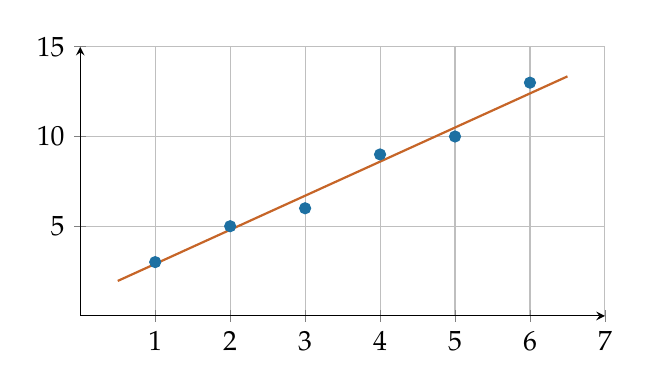
\begin{tikzpicture}\begin{axis}[width=.68\textwidth,height=5cm,axis lines=middle,xmin=0,xmax=7,ymin=0,ymax=15,grid=major]\addplot[only marks,Blue,mark=*] coordinates {(1,3)(2,5)(3,6)(4,9)(5,10)(6,13)};\addplot[Orange,thick,domain=.5:6.5]{1.9*x+1};\end{axis}\end{tikzpicture}\end{center}
\end{activite}
\enseignant{$y=35$ et $x=7{,}5$. Les deux valeurs sont à l'intérieur de l'intervalle observé : interpolations. Faire verbaliser la donnée qui déclenche le choix de méthode.}

\begin{traceecrite}Une interpolation estime une valeur à l'intérieur de l'intervalle observé. Le résultat est une estimation dépendante du modèle.\end{traceecrite}

\begin{exemple}
Reprendre les données de l'activité et rédiger la solution dans l'ordre : définition des objets, propriété utilisée, calcul exact ou approché, puis phrase de réponse. La réponse modèle figure dans l'édition enseignant.
\end{exemple}
\enseignant{$y=35$ et $x=7{,}5$. Les deux valeurs sont à l'intérieur de l'intervalle observé : interpolations.}

\begin{exercice}[-- essentiel]
\begin{enumerate}\item Pour $y=6x+16$, estimer $y$ lorsque $x=8$.\item Résoudre $6x+16=50$.\item Le modèle a été établi sur $[2,12]$ : qualifier les estimations pour $x=8$ et $x=30$.\end{enumerate}
\end{exercice}
\enseignant{Pour $x=8$, $y=64$. L'équation donne $x=\dfrac{34}{6}$. $x=8$ donne une interpolation ; $x=30$ une extrapolation.}

\manuelref{Calao, p. 118, n° 19 à 24}
\CalaoSession{34}

\begin{dm}Reprendre l'exercice d'entraînement 3 avec les données suivantes : remplacer la donnée initiale par $290$ et le taux ou la raison par $6$. Rédiger en quatre lignes : données, formule, calcul, conclusion.\end{dm}
\enseignant{La correction dépend de l'exercice repris. Vérifier surtout la cohérence du modèle, le nombre d'itérations, l'arrondi et la phrase de conclusion.}

\begin{sortie}Sur une demi-feuille : écrire la règle principale de la séance, traiter un exemple très court et indiquer son degré de confiance de 1 à 4. Question(s) essentielle(s) du jour : 1 et 2.\end{sortie}

\ifprof
\begin{methode}
\textbf{Conduite en 1 h :} 7 min d'automatismes ; 10 min de mise en commun et trace ; 28 min d'exercices essentiels ; 5 min de correction ; 3 min de billet de sortie.\\
\textbf{Conduite en 2 h :} ajouter 20 min de recherche de l'activité, 20 min d'institutionnalisation, un second exercice autonome et 10 min de correction comparée.\\
\textbf{Différenciation :} fournir aux élèves fragiles une fiche à quatre cases (données, modèle, calcul, conclusion). Demander aux élèves rapides de produire un contre-exemple, une justification ou une seconde méthode.
\end{methode}
\fi
\sessionheader{35}{09/02/2027}{B : 2 h -- C : 1 h}{Extrapolation}{Statistiques à deux variables}
\begin{objectifs}\begin{itemize}\item Extrapoler prudemment.\item Évaluer la plausibilité.\item Présenter une limite du modèle.\end{itemize}\end{objectifs}
\begin{automatismes}\begin{enumerate}\item Réduire $3x+3-x+2$. \rep{$2x+5$}\item Résoudre $3x+4=25$. \rep{$x=7$}\item Calculer la moyenne de $3$, $5$ et $7$. \rep{$5$}\item Donner la pente entre $(1,3)$ et $(4,9)$. \rep{$\dfrac{9-3}{4-1}=2$}\item Avec $y=2x+5$, calculer $y$ pour $x=7$. \rep{$19$}\end{enumerate}\end{automatismes}
\begin{prerequis}Relire la dernière trace écrite et savoir effectuer les calculs élémentaires mobilisés aujourd'hui. Avant l'activité, faire reformuler les mots-clés : extrapoler prudemment et évaluer la plausibilité.\end{prerequis}

\begin{activite}
Le même modèle $y=2{,}8x+14$, ajusté sur $[1,12]$, est utilisé pour $x=40$. Calculer l'estimation, puis donner trois raisons pour lesquelles elle peut être peu fiable.
\begin{center}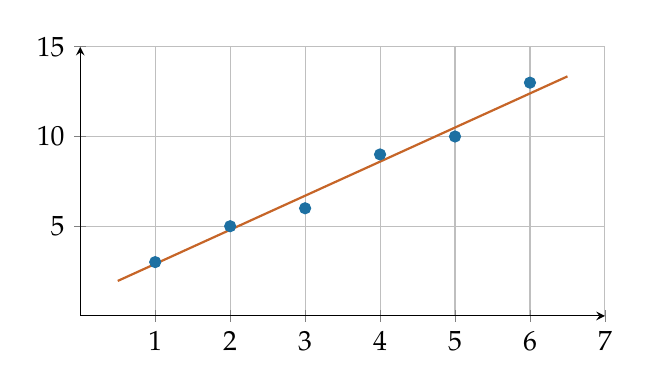
\begin{tikzpicture}\begin{axis}[width=.68\textwidth,height=5cm,axis lines=middle,xmin=0,xmax=7,ymin=0,ymax=15,grid=major]\addplot[only marks,Blue,mark=*] coordinates {(1,3)(2,5)(3,6)(4,9)(5,10)(6,13)};\addplot[Orange,thick,domain=.5:6.5]{1.9*x+1};\end{axis}\end{tikzpicture}\end{center}
\end{activite}
\enseignant{L'estimation vaut $126$. Elle est éloignée des données, la tendance peut changer et des contraintes réelles peuvent plafonner la variable. Faire verbaliser la donnée qui déclenche le choix de méthode.}

\begin{traceecrite}Une extrapolation estime hors de l'intervalle observé. Plus on s'en éloigne, plus la prudence est nécessaire.\end{traceecrite}

\begin{exemple}
Reprendre les données de l'activité et rédiger la solution dans l'ordre : définition des objets, propriété utilisée, calcul exact ou approché, puis phrase de réponse. La réponse modèle figure dans l'édition enseignant.
\end{exemple}
\enseignant{L'estimation vaut $126$. Elle est éloignée des données, la tendance peut changer et des contraintes réelles peuvent plafonner la variable.}

\begin{exercice}[-- essentiel]
\begin{enumerate}\item Pour $y=2x+12$, estimer $y$ lorsque $x=8$.\item Résoudre $2x+12=50$.\item Le modèle a été établi sur $[2,12]$ : qualifier les estimations pour $x=8$ et $x=30$.\end{enumerate}
\end{exercice}
\enseignant{Pour $x=8$, $y=28$. L'équation donne $x=\dfrac{38}{2}$. $x=8$ donne une interpolation ; $x=30$ une extrapolation.}

\manuelref{Calao, p. 119, n° 25 à 27}
\CalaoSession{35}

\begin{dm}Reprendre l'exercice d'entraînement 2 avec les données suivantes : remplacer la donnée initiale par $295$ et le taux ou la raison par $7$. Rédiger en quatre lignes : données, formule, calcul, conclusion.\end{dm}
\enseignant{La correction dépend de l'exercice repris. Vérifier surtout la cohérence du modèle, le nombre d'itérations, l'arrondi et la phrase de conclusion.}

\begin{sortie}Sur une demi-feuille : écrire la règle principale de la séance, traiter un exemple très court et indiquer son degré de confiance de 1 à 4. Question(s) essentielle(s) du jour : 1, 2 et 3.\end{sortie}

\ifprof
\begin{methode}
\textbf{Conduite en 1 h :} 7 min d'automatismes ; 10 min de mise en commun et trace ; 28 min d'exercices essentiels ; 5 min de correction ; 3 min de billet de sortie.\\
\textbf{Conduite en 2 h :} ajouter 20 min de recherche de l'activité, 20 min d'institutionnalisation, un second exercice autonome et 10 min de correction comparée.\\
\textbf{Différenciation :} fournir aux élèves fragiles une fiche à quatre cases (données, modèle, calcul, conclusion). Demander aux élèves rapides de produire un contre-exemple, une justification ou une seconde méthode.
\end{methode}
\fi
\sessionheader{36}{11/02/2027}{B : 1 h -- C : 2 h}{Changement de variable}{Statistiques à deux variables}
\begin{objectifs}\begin{itemize}\item Effectuer un changement de variable.\item Ajuster les nouvelles données.\item Revenir à la variable initiale.\end{itemize}\end{objectifs}
\begin{automatismes}\begin{enumerate}\item Calculer $5\,\%$ de $80$. \rep{$4$}\item Calculer la moyenne de $4$, $6$ et $8$. \rep{$6$}\item Donner la pente entre $(1,3)$ et $(4,9)$. \rep{$\dfrac{9-3}{4-1}=2$}\item Avec $y=2x+5$, calculer $y$ pour $x=7$. \rep{$19$}\item Résoudre $3x+4=25$. \rep{$x=7$}\end{enumerate}\end{automatismes}
\begin{prerequis}Relire la dernière trace écrite et savoir effectuer les calculs élémentaires mobilisés aujourd'hui. Avant l'activité, faire reformuler les mots-clés : effectuer un changement de variable et ajuster les nouvelles données.\end{prerequis}

\begin{activite}
Les données semblent exponentielles. On pose $z=\log(y)$ et l'ajustement donne $z=0{,}08x+1{,}2$. Exprimer $y$ en fonction de $x$, puis calculer $y$ pour $x=5$.

\end{activite}
\enseignant{$y=10^{0{,}08x+1{,}2}$. Pour $x=5$, $y=10^{1{,}6}\approx39{,}8$. Faire verbaliser la donnée qui déclenche le choix de méthode.}

\begin{traceecrite}Un changement de variable peut aligner un nuage. Après l'ajustement dans la nouvelle variable, il faut revenir à la variable initiale.\end{traceecrite}

\begin{exemple}
Reprendre les données de l'activité et rédiger la solution dans l'ordre : définition des objets, propriété utilisée, calcul exact ou approché, puis phrase de réponse. La réponse modèle figure dans l'édition enseignant.
\end{exemple}
\enseignant{$y=10^{0{,}08x+1{,}2}$. Pour $x=5$, $y=10^{1{,}6}\approx39{,}8$.}

\begin{exercice}[-- essentiel]
\begin{enumerate}\item Pour $y=3x+13$, estimer $y$ lorsque $x=8$.\item Résoudre $3x+13=50$.\item Le modèle a été établi sur $[2,12]$ : qualifier les estimations pour $x=8$ et $x=30$.\end{enumerate}
\end{exercice}
\enseignant{Pour $x=8$, $y=37$. L'équation donne $x=\dfrac{37}{3}$. $x=8$ donne une interpolation ; $x=30$ une extrapolation.}

\manuelref{Calao, p. 120, n° 28--29}
\CalaoSession{36}

\begin{dm}Reprendre l'exercice d'entraînement 3 avec les données suivantes : remplacer la donnée initiale par $300$ et le taux ou la raison par $2$. Rédiger en quatre lignes : données, formule, calcul, conclusion.\end{dm}
\enseignant{La correction dépend de l'exercice repris. Vérifier surtout la cohérence du modèle, le nombre d'itérations, l'arrondi et la phrase de conclusion.}

\begin{sortie}Sur une demi-feuille : écrire la règle principale de la séance, traiter un exemple très court et indiquer son degré de confiance de 1 à 4. Question(s) essentielle(s) du jour : 1 et 2.\end{sortie}

\ifprof
\begin{methode}
\textbf{Conduite en 1 h :} 7 min d'automatismes ; 10 min de mise en commun et trace ; 28 min d'exercices essentiels ; 5 min de correction ; 3 min de billet de sortie.\\
\textbf{Conduite en 2 h :} ajouter 20 min de recherche de l'activité, 20 min d'institutionnalisation, un second exercice autonome et 10 min de correction comparée.\\
\textbf{Différenciation :} fournir aux élèves fragiles une fiche à quatre cases (données, modèle, calcul, conclusion). Demander aux élèves rapides de produire un contre-exemple, une justification ou une seconde méthode.
\end{methode}
\fi
\sessionheader{37}{02/03/2027}{B : 2 h -- C : 1 h}{Choix du modèle et ajustement}{Statistiques à deux variables}
\begin{objectifs}\begin{itemize}\item Comparer des modèles.\item Utiliser les résidus.\item Définir un domaine d'usage.\end{itemize}\end{objectifs}
\begin{automatismes}\begin{enumerate}\item Écrire le coefficient multiplicateur d'une hausse de $10\,\%$. \rep{$1+\dfrac{10}{100}=1,10$}\item Donner la pente entre $(1,3)$ et $(4,9)$. \rep{$\dfrac{9-3}{4-1}=2$}\item Avec $y=2x+5$, calculer $y$ pour $x=7$. \rep{$19$}\item Résoudre $3x+4=25$. \rep{$x=7$}\item Calculer la moyenne de $5$, $7$ et $9$. \rep{$7$}\end{enumerate}\end{automatismes}
\begin{prerequis}Relire la dernière trace écrite et savoir effectuer les calculs élémentaires mobilisés aujourd'hui. Avant l'activité, faire reformuler les mots-clés : comparer des modèles et utiliser les résidus.\end{prerequis}

\begin{activite}
Deux modèles donnent des résidus absolus totaux $18{,}4$ et $11{,}7$ sur la zone observée. Le second comporte cependant une croissance irréaliste après $x=20$. Choisir un modèle pour interpoler à $x=12$, puis discuter l'extrapolation à $x=50$.
\begin{center}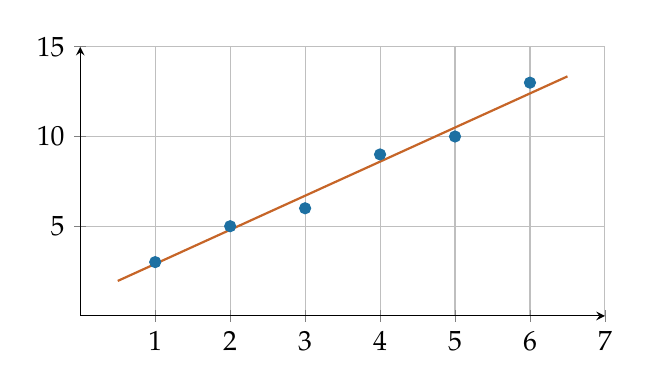
\begin{tikzpicture}\begin{axis}[width=.68\textwidth,height=5cm,axis lines=middle,xmin=0,xmax=7,ymin=0,ymax=15,grid=major]\addplot[only marks,Blue,mark=*] coordinates {(1,3)(2,5)(3,6)(4,9)(5,10)(6,13)};\addplot[Orange,thick,domain=.5:6.5]{1.9*x+1};\end{axis}\end{tikzpicture}\end{center}
\end{activite}
\enseignant{Le second est préférable pour interpoler sur la zone observée si les autres critères sont comparables ; aucun choix automatique n'est justifié pour $x=50$. Faire verbaliser la donnée qui déclenche le choix de méthode.}

\begin{traceecrite}On choisit un modèle selon la forme du nuage, la taille des résidus et le domaine d'usage. Un meilleur ajustement visuel n'autorise pas une extrapolation illimitée.\end{traceecrite}

\begin{exemple}
Reprendre les données de l'activité et rédiger la solution dans l'ordre : définition des objets, propriété utilisée, calcul exact ou approché, puis phrase de réponse. La réponse modèle figure dans l'édition enseignant.
\end{exemple}
\enseignant{Le second est préférable pour interpoler sur la zone observée si les autres critères sont comparables ; aucun choix automatique n'est justifié pour $x=50$.}

\begin{exercice}[-- essentiel]
\begin{enumerate}\item Pour $y=4x+14$, estimer $y$ lorsque $x=8$.\item Résoudre $4x+14=50$.\item Le modèle a été établi sur $[2,12]$ : qualifier les estimations pour $x=8$ et $x=30$.\end{enumerate}
\end{exercice}
\enseignant{Pour $x=8$, $y=46$. L'équation donne $x=\dfrac{36}{4}$. $x=8$ donne une interpolation ; $x=30$ une extrapolation.}

\manuelref{Calao, p. 121, n° 30 à 32, puis p. 122, n° 33}
\CalaoSession{37}

\begin{dm}Reprendre l'exercice d'entraînement 2 avec les données suivantes : remplacer la donnée initiale par $305$ et le taux ou la raison par $3$. Rédiger en quatre lignes : données, formule, calcul, conclusion.\end{dm}
\enseignant{La correction dépend de l'exercice repris. Vérifier surtout la cohérence du modèle, le nombre d'itérations, l'arrondi et la phrase de conclusion.}

\begin{sortie}Sur une demi-feuille : écrire la règle principale de la séance, traiter un exemple très court et indiquer son degré de confiance de 1 à 4. Question(s) essentielle(s) du jour : 1, 2 et 3.\end{sortie}

\ifprof
\begin{methode}
\textbf{Conduite en 1 h :} 7 min d'automatismes ; 10 min de mise en commun et trace ; 28 min d'exercices essentiels ; 5 min de correction ; 3 min de billet de sortie.\\
\textbf{Conduite en 2 h :} ajouter 20 min de recherche de l'activité, 20 min d'institutionnalisation, un second exercice autonome et 10 min de correction comparée.\\
\textbf{Différenciation :} fournir aux élèves fragiles une fiche à quatre cases (données, modèle, calcul, conclusion). Demander aux élèves rapides de produire un contre-exemple, une justification ou une seconde méthode.
\end{methode}
\fi
\sessionheader{38}{04/03/2027}{B : 1 h -- C : 2 h}{Bilan et évaluation}{Statistiques à deux variables}
\begin{objectifs}\begin{itemize}\item Choisir et exploiter un ajustement.\item Rédiger une conclusion statistique.\item Analyser une erreur.\end{itemize}\end{objectifs}
\begin{automatismes}\begin{enumerate}\item Réduire $3x+6-x+2$. \rep{$2x+8$}\item Avec $y=2x+5$, calculer $y$ pour $x=7$. \rep{$19$}\item Résoudre $3x+4=25$. \rep{$x=7$}\item Calculer la moyenne de $6$, $8$ et $10$. \rep{$8$}\item Donner la pente entre $(1,3)$ et $(4,9)$. \rep{$\dfrac{9-3}{4-1}=2$}\end{enumerate}\end{automatismes}
\begin{prerequis}Relire la dernière trace écrite et savoir effectuer les calculs élémentaires mobilisés aujourd'hui. Avant l'activité, faire reformuler les mots-clés : choisir et exploiter un ajustement et rédiger une conclusion statistique.\end{prerequis}

\begin{activite}
À partir d'un nuage fourni par le professeur, produire une réponse complète : choix du modèle, équation, estimation, type d'estimation, unité et réserve. Échanger les copies et utiliser une grille de six critères.

\end{activite}
\enseignant{La correction vérifie la cohérence du modèle et la présence des six éléments demandés, pas seulement le résultat numérique. Faire verbaliser la donnée qui déclenche le choix de méthode.}

\begin{traceecrite}Une réponse statistique complète contient le modèle, le calcul, l'arrondi, l'unité, le type d'estimation et une réserve sur la validité.\end{traceecrite}

\begin{exemple}
Reprendre les données de l'activité et rédiger la solution dans l'ordre : définition des objets, propriété utilisée, calcul exact ou approché, puis phrase de réponse. La réponse modèle figure dans l'édition enseignant.
\end{exemple}
\enseignant{La correction vérifie la cohérence du modèle et la présence des six éléments demandés, pas seulement le résultat numérique.}

\begin{exercice}[-- essentiel]
\begin{enumerate}\item Pour $y=5x+15$, estimer $y$ lorsque $x=8$.\item Résoudre $5x+15=50$.\item Le modèle a été établi sur $[2,12]$ : qualifier les estimations pour $x=8$ et $x=30$.\end{enumerate}
\end{exercice}
\enseignant{Pour $x=8$, $y=55$. L'équation donne $x=\dfrac{35}{5}$. $x=8$ donne une interpolation ; $x=30$ une extrapolation.}

\manuelref{Calao, p. 122--123}
\CalaoSession{38}

\begin{dm}Reprendre l'exercice d'entraînement 3 avec les données suivantes : remplacer la donnée initiale par $310$ et le taux ou la raison par $4$. Rédiger en quatre lignes : données, formule, calcul, conclusion.\end{dm}
\enseignant{La correction dépend de l'exercice repris. Vérifier surtout la cohérence du modèle, le nombre d'itérations, l'arrondi et la phrase de conclusion.}

\begin{sortie}Sur une demi-feuille : écrire la règle principale de la séance, traiter un exemple très court et indiquer son degré de confiance de 1 à 4. Question(s) essentielle(s) du jour : 1 et 2.\end{sortie}

\ifprof
\begin{methode}
\textbf{Conduite en 1 h :} 7 min d'automatismes ; 10 min de mise en commun et trace ; 28 min d'exercices essentiels ; 5 min de correction ; 3 min de billet de sortie.\\
\textbf{Conduite en 2 h :} ajouter 20 min de recherche de l'activité, 20 min d'institutionnalisation, un second exercice autonome et 10 min de correction comparée.\\
\textbf{Différenciation :} fournir aux élèves fragiles une fiche à quatre cases (données, modèle, calcul, conclusion). Demander aux élèves rapides de produire un contre-exemple, une justification ou une seconde méthode.
\end{methode}
\fi


\chapter{Probabilités conditionnelles}
\competences{modéliser par un arbre ou un tableau, calculer, raisonner sur l'indépendance, interpréter}
\section{Cours de référence}
Pour deux événements $A$ et $B$ avec $P(A)>0$, la probabilité de $B$ sachant $A$ est
\[
P_A(B)=P(B\mid A)=\frac{P(A\cap B)}{P(A)}.
\]

\begin{center}
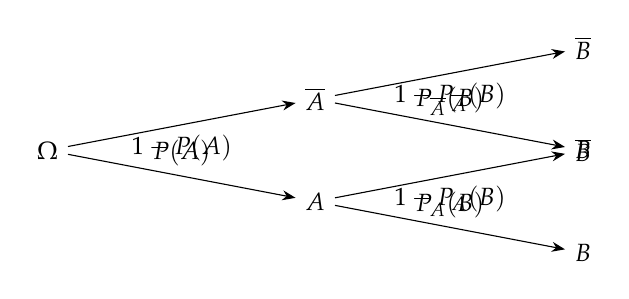
\begin{tikzpicture}[grow=right,level distance=34mm,sibling distance=13mm,every node/.style={font=\small},edge from parent/.style={draw,-{Stealth}}]
\node {$\Omega$}
 child {node {$A$}
   child {node {$B$} edge from parent node[above] {$P_A(B)$}}
   child {node {$\overline B$} edge from parent node[below] {$1-P_A(B)$}}
   edge from parent node[above] {$P(A)$}}
 child {node {$\overline A$}
   child {node {$B$} edge from parent node[above] {$P_{\overline A}(B)$}}
   child {node {$\overline B$} edge from parent node[below] {$1-P_{\overline A}(B)$}}
   edge from parent node[below] {$1-P(A)$}};
\end{tikzpicture}
\end{center}

\begin{retenir}
Dans un arbre pondéré, les probabilités issues d'un même nœud ont pour somme $1$. On multiplie les probabilités le long d'un chemin : $P(A\cap B)=P(A)P_A(B)$. On additionne les probabilités de chemins incompatibles menant à l'événement recherché.
\end{retenir}

Si $A_1,\ldots,A_n$ forment une partition de l'univers, alors
\[
P(B)=P(A_1)P_{A_1}(B)+\cdots+P(A_n)P_{A_n}(B).
\]
Deux événements $A$ et $B$ de probabilités non nulles sont indépendants si $P(A\cap B)=P(A)P(B)$, ou de manière équivalente si $P_A(B)=P(B)$.

\begin{erreur}
Ne pas confondre $P_A(B)$ et $P_B(A)$. La condition figure après le mot « sachant » et se place en indice dans la notation française.
\end{erreur}

\begin{exemple}
$40\,\%$ des clients achètent en ligne. Parmi eux, $12\,\%$ retournent leur commande ; parmi les autres, $5\,\%$ la retournent. Alors $P(R)=0{,}40\times0{,}12+0{,}60\times0{,}05=0{,}078$. Le taux global de retour est donc $7{,}8\,\%$.
\end{exemple}

\sessionheader{39}{09/03/2027}{B : 2 h -- C : 1 h}{Conditionnement}{Probabilités conditionnelles}
\begin{objectifs}\begin{itemize}\item Définir une probabilité conditionnelle.\item Passer des effectifs aux probabilités.\item Interpréter.\end{itemize}\end{objectifs}
\begin{automatismes}\begin{enumerate}\item Calculer $20\,\%$ de $140$. \rep{$28$}\item Que vaut la somme des branches issues d'un nœud ? \rep{$1$}\item Calculer $0{,}7\times0{,}4$. \rep{$0,28$}\item Si $P(A)=0{,}37$, calculer $P(\overline A)$. \rep{$0{,}63$}\item Simplifier $\dfrac{18}{30}$. \rep{$\dfrac35$}\end{enumerate}\end{automatismes}
\begin{prerequis}Relire la dernière trace écrite et savoir effectuer les calculs élémentaires mobilisés aujourd'hui. Avant l'activité, faire reformuler les mots-clés : définir une probabilité conditionnelle et passer des effectifs aux probabilités.\end{prerequis}

\begin{activite}
Dans une enquête, $180$ clients sur $600$ utilisent une carte premium et $72$ de ces $180$ clients achètent chaque semaine. Calculer $P(P)$, $P(P\cap H)$ et $P_P(H)$, puis interpréter.

\end{activite}
\enseignant{$P(P)=0{,}30$, $P(P\cap H)=0{,}12$ et $P_P(H)=\dfrac{72}{180}=0{,}40$. Faire verbaliser la donnée qui déclenche le choix de méthode.}

\begin{traceecrite}Pour $P(A)>0$, $P_A(B)=\dfrac{P(A\cap B)}{P(A)}$. Il s'agit de la probabilité de $B$ dans la population restreinte à $A$.\end{traceecrite}

\begin{exemple}
Reprendre les données de l'activité et rédiger la solution dans l'ordre : définition des objets, propriété utilisée, calcul exact ou approché, puis phrase de réponse. La réponse modèle figure dans l'édition enseignant.
\end{exemple}
\enseignant{$P(P)=0{,}30$, $P(P\cap H)=0{,}12$ et $P_P(H)=\dfrac{72}{180}=0{,}40$.}

\begin{exercice}[-- essentiel]
\begin{enumerate}\item On sait $P(A)=0{,}35$, $P_A(B)=0{,}6$ et $P_{\overline A}(B)=0{,}8$. Construire l'arbre.\item Calculer $P(A\cap B)$ puis $P(B)$.\item Calculer $P_B(A)$ et tester l'indépendance.\end{enumerate}
\end{exercice}
\enseignant{$P(A\cap B)=0{,}35\times0{,}6$. Puis $P(B)=P(A)P_A(B)+(1-P(A))P_{\overline A}(B)$ et $P_B(A)=\dfrac{P(A\cap B)}{P(B)}$. Comparer à $P(A)$.}

\manuelref{Calao, cours p. 132--137 ; exercices p. 138, n° 1 à 5}
\ExoSession{39}

\begin{dm}Reprendre l'exercice d'entraînement 2 avec les données suivantes : remplacer la donnée initiale par $315$ et le taux ou la raison par $5$. Rédiger en quatre lignes : données, formule, calcul, conclusion.\end{dm}
\enseignant{La correction dépend de l'exercice repris. Vérifier surtout la cohérence du modèle, le nombre d'itérations, l'arrondi et la phrase de conclusion.}

\begin{sortie}Sur une demi-feuille : écrire la règle principale de la séance, traiter un exemple très court et indiquer son degré de confiance de 1 à 4. Question(s) essentielle(s) du jour : 1, 2 et 3.\end{sortie}

\ifprof
\begin{methode}
\textbf{Conduite en 1 h :} 7 min d'automatismes ; 10 min de mise en commun et trace ; 28 min d'exercices essentiels ; 5 min de correction ; 3 min de billet de sortie.\\
\textbf{Conduite en 2 h :} ajouter 20 min de recherche de l'activité, 20 min d'institutionnalisation, un second exercice autonome et 10 min de correction comparée.\\
\textbf{Différenciation :} fournir aux élèves fragiles une fiche à quatre cases (données, modèle, calcul, conclusion). Demander aux élèves rapides de produire un contre-exemple, une justification ou une seconde méthode.
\end{methode}
\fi
\sessionheader{40}{11/03/2027}{B : 1 h -- C : 2 h}{Arbres pondérés}{Probabilités conditionnelles}
    \begin{objectifs}\begin{itemize}\item Construire et compléter un arbre.\item Lire une probabilité conditionnelle.\item Contrôler les sommes.\end{itemize}\end{objectifs}
    \begin{automatismes}\begin{enumerate}\item Écrire le coefficient multiplicateur d'une hausse de $25\,\%$. \rep{$1+\dfrac{25}{100}=1,25$}\item Calculer $0{,}8\times0{,}4$. \rep{$0,32$}\item Si $P(A)=0{,}37$, calculer $P(\overline A)$. \rep{$0{,}63$}\item Simplifier $\dfrac{18}{30}$. \rep{$\dfrac35$}\item Que vaut la somme des branches issues d'un nœud ? \rep{$1$}\end{enumerate}\end{automatismes}
    \begin{prerequis}Relire la dernière trace écrite et savoir effectuer les calculs élémentaires mobilisés aujourd'hui. Avant l'activité, faire reformuler les mots-clés : construire et compléter un arbre et lire une probabilité conditionnelle.\end{prerequis}

    \begin{activite}
    $35\,\%$ des commandes sont express. Parmi elles, $4\,\%$ sont en retard ; parmi les commandes standard, $9\,\%$ sont en retard. Construire et compléter l'arbre.
    \begin{center}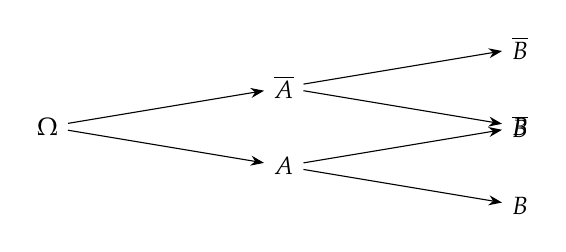
\begin{tikzpicture}[grow=right,level distance=30mm,sibling distance=10mm,every node/.style={font=\small},edge from parent/.style={draw,-{Stealth}}]
\node {$\Omega$} child {node {$A$} child {node {$B$}} child {node {$\overline B$}}} child {node {$\overline A$} child {node {$B$}} child {node {$\overline B$}}};
\end{tikzpicture}\end{center}
    \end{activite}
    \enseignant{Premières branches : $0{,}35$ et $0{,}65$. Puis $0{,}04$ et $0{,}96$ ; enfin $0{,}09$ et $0{,}91$. Faire verbaliser la donnée qui déclenche le choix de méthode.}

    \begin{traceecrite}Dans un arbre, les branches issues d'un nœud ont pour somme $1$. Les probabilités de second niveau sont conditionnelles.\end{traceecrite}

    \begin{exemple}
    Reprendre les données de l'activité et rédiger la solution dans l'ordre : définition des objets, propriété utilisée, calcul exact ou approché, puis phrase de réponse. La réponse modèle figure dans l'édition enseignant.
    \end{exemple}
    \enseignant{Premières branches : $0{,}35$ et $0{,}65$. Puis $0{,}04$ et $0{,}96$ ; enfin $0{,}09$ et $0{,}91$.}

    \begin{exercice}[-- essentiel]
    \begin{enumerate}\item On sait $P(A)=0{,}40$, $P_A(B)=0{,}2$ et $P_{\overline A}(B)=0{,}4$. Construire l'arbre.\item Calculer $P(A\cap B)$ puis $P(B)$.\item Calculer $P_B(A)$ et tester l'indépendance.\end{enumerate}
    \end{exercice}
    \enseignant{$P(A\cap B)=0{,}40\times0{,}2$. Puis $P(B)=P(A)P_A(B)+(1-P(A))P_{\overline A}(B)$ et $P_B(A)=\dfrac{P(A\cap B)}{P(B)}$. Comparer à $P(A)$.}

    \manuelref{Calao, cours p. 133--137 ; exercices p. 140, n° 14 à 18}
\ExoSession{40}

    \begin{dm}Reprendre l'exercice d'entraînement 3 avec les données suivantes : remplacer la donnée initiale par $320$ et le taux ou la raison par $6$. Rédiger en quatre lignes : données, formule, calcul, conclusion.\end{dm}
    \enseignant{La correction dépend de l'exercice repris. Vérifier surtout la cohérence du modèle, le nombre d'itérations, l'arrondi et la phrase de conclusion.}

    \begin{sortie}Sur une demi-feuille : écrire la règle principale de la séance, traiter un exemple très court et indiquer son degré de confiance de 1 à 4. Question(s) essentielle(s) du jour : 1 et 2.\end{sortie}

    \ifprof
    \begin{methode}
    \textbf{Conduite en 1 h :} 7 min d'automatismes ; 10 min de mise en commun et trace ; 28 min d'exercices essentiels ; 5 min de correction ; 3 min de billet de sortie.\\
    \textbf{Conduite en 2 h :} ajouter 20 min de recherche de l'activité, 20 min d'institutionnalisation, un second exercice autonome et 10 min de correction comparée.\\
    \textbf{Différenciation :} fournir aux élèves fragiles une fiche à quatre cases (données, modèle, calcul, conclusion). Demander aux élèves rapides de produire un contre-exemple, une justification ou une seconde méthode.
    \end{methode}
    \fi
\sessionheader{41}{16/03/2027}{B : 2 h -- C : 1 h}{Produit des probabilités le long d'un chemin}{Probabilités conditionnelles}
    \begin{objectifs}\begin{itemize}\item Calculer une intersection.\item Combiner les chemins.\item Traduire un événement.\end{itemize}\end{objectifs}
    \begin{automatismes}\begin{enumerate}\item Réduire $3x+9-x+2$. \rep{$2x+11$}\item Si $P(A)=0{,}37$, calculer $P(\overline A)$. \rep{$0{,}63$}\item Simplifier $\dfrac{18}{30}$. \rep{$\dfrac35$}\item Que vaut la somme des branches issues d'un nœud ? \rep{$1$}\item Calculer $0{,}9\times0{,}4$. \rep{$0,36$}\end{enumerate}\end{automatismes}
    \begin{prerequis}Relire la dernière trace écrite et savoir effectuer les calculs élémentaires mobilisés aujourd'hui. Avant l'activité, faire reformuler les mots-clés : calculer une intersection et combiner les chemins.\end{prerequis}

    \begin{activite}
    Avec l'arbre de la séance 40, calculer la probabilité d'une commande express et en retard, puis la probabilité totale d'un retard. Interpréter les deux résultats.
    \begin{center}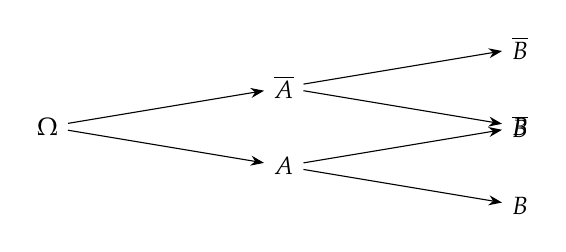
\begin{tikzpicture}[grow=right,level distance=30mm,sibling distance=10mm,every node/.style={font=\small},edge from parent/.style={draw,-{Stealth}}]
\node {$\Omega$} child {node {$A$} child {node {$B$}} child {node {$\overline B$}}} child {node {$\overline A$} child {node {$B$}} child {node {$\overline B$}}};
\end{tikzpicture}\end{center}
    \end{activite}
    \enseignant{$P(E\cap R)=0{,}35\times0{,}04=0{,}014$. $P(R)=0{,}014+0{,}65\times0{,}09=0{,}0725$. Faire verbaliser la donnée qui déclenche le choix de méthode.}

    \begin{traceecrite}On multiplie le long d'un chemin : $P(A\cap B)=P(A)P_A(B)$. On additionne les chemins incompatibles qui réalisent l'événement.\end{traceecrite}

    \begin{exemple}
    Reprendre les données de l'activité et rédiger la solution dans l'ordre : définition des objets, propriété utilisée, calcul exact ou approché, puis phrase de réponse. La réponse modèle figure dans l'édition enseignant.
    \end{exemple}
    \enseignant{$P(E\cap R)=0{,}35\times0{,}04=0{,}014$. $P(R)=0{,}014+0{,}65\times0{,}09=0{,}0725$.}

    \begin{exercice}[-- essentiel]
    \begin{enumerate}\item On sait $P(A)=0{,}45$, $P_A(B)=0{,}3$ et $P_{\overline A}(B)=0{,}5$. Construire l'arbre.\item Calculer $P(A\cap B)$ puis $P(B)$.\item Calculer $P_B(A)$ et tester l'indépendance.\end{enumerate}
    \end{exercice}
    \enseignant{$P(A\cap B)=0{,}45\times0{,}3$. Puis $P(B)=P(A)P_A(B)+(1-P(A))P_{\overline A}(B)$ et $P_B(A)=\dfrac{P(A\cap B)}{P(B)}$. Comparer à $P(A)$.}

    \manuelref{Calao, p. 140, n° 14 à 18}
\ExoSession{41}

    \begin{dm}Reprendre l'exercice d'entraînement 2 avec les données suivantes : remplacer la donnée initiale par $325$ et le taux ou la raison par $7$. Rédiger en quatre lignes : données, formule, calcul, conclusion.\end{dm}
    \enseignant{La correction dépend de l'exercice repris. Vérifier surtout la cohérence du modèle, le nombre d'itérations, l'arrondi et la phrase de conclusion.}

    \begin{sortie}Sur une demi-feuille : écrire la règle principale de la séance, traiter un exemple très court et indiquer son degré de confiance de 1 à 4. Question(s) essentielle(s) du jour : 1, 2 et 3.\end{sortie}

    \ifprof
    \begin{methode}
    \textbf{Conduite en 1 h :} 7 min d'automatismes ; 10 min de mise en commun et trace ; 28 min d'exercices essentiels ; 5 min de correction ; 3 min de billet de sortie.\\
    \textbf{Conduite en 2 h :} ajouter 20 min de recherche de l'activité, 20 min d'institutionnalisation, un second exercice autonome et 10 min de correction comparée.\\
    \textbf{Différenciation :} fournir aux élèves fragiles une fiche à quatre cases (données, modèle, calcul, conclusion). Demander aux élèves rapides de produire un contre-exemple, une justification ou une seconde méthode.
    \end{methode}
    \fi
\sessionheader{42}{18/03/2027}{B : 1 h -- C : 2 h}{Indépendance}{Probabilités conditionnelles}
\begin{objectifs}\begin{itemize}\item Tester l'indépendance.\item Comparer probabilités.\item Justifier une conclusion.\end{itemize}\end{objectifs}
\begin{automatismes}\begin{enumerate}\item Calculer $5\,\%$ de $60$. \rep{$3$}\item Simplifier $\dfrac{18}{30}$. \rep{$\dfrac35$}\item Que vaut la somme des branches issues d'un nœud ? \rep{$1$}\item Calculer $0{,}3\times0{,}4$. \rep{$0,12$}\item Si $P(A)=0{,}37$, calculer $P(\overline A)$. \rep{$0{,}63$}\end{enumerate}\end{automatismes}
\begin{prerequis}Relire la dernière trace écrite et savoir effectuer les calculs élémentaires mobilisés aujourd'hui. Avant l'activité, faire reformuler les mots-clés : tester l'indépendance et comparer probabilités.\end{prerequis}

\begin{activite}
Dans une population, $P(A)=0{,}4$, $P(B)=0{,}3$ et $P(A\cap B)=0{,}12$. Tester l'indépendance de deux façons. Modifier ensuite $P(A\cap B)$ en $0{,}15$ et recommencer.

\end{activite}
\enseignant{$0{,}4\times0{,}3=0{,}12$ : indépendance. Avec $0{,}15$, les événements ne sont plus indépendants. Faire verbaliser la donnée qui déclenche le choix de méthode.}

\begin{traceecrite}$A$ et $B$ sont indépendants si $P(A\cap B)=P(A)P(B)$, équivalemment si $P_A(B)=P(B)$ lorsque $P(A)>0$.\end{traceecrite}

\begin{exemple}
Reprendre les données de l'activité et rédiger la solution dans l'ordre : définition des objets, propriété utilisée, calcul exact ou approché, puis phrase de réponse. La réponse modèle figure dans l'édition enseignant.
\end{exemple}
\enseignant{$0{,}4\times0{,}3=0{,}12$ : indépendance. Avec $0{,}15$, les événements ne sont plus indépendants.}

\begin{exercice}[-- essentiel]
\begin{enumerate}\item On sait $P(A)=0{,}20$, $P_A(B)=0{,}4$ et $P_{\overline A}(B)=0{,}6$. Construire l'arbre.\item Calculer $P(A\cap B)$ puis $P(B)$.\item Calculer $P_B(A)$ et tester l'indépendance.\end{enumerate}
\end{exercice}
\enseignant{$P(A\cap B)=0{,}20\times0{,}4$. Puis $P(B)=P(A)P_A(B)+(1-P(A))P_{\overline A}(B)$ et $P_B(A)=\dfrac{P(A\cap B)}{P(B)}$. Comparer à $P(A)$.}

\manuelref{Calao, cours p. 134--137 ; exercices p. 144, n° 33 à 35}
\ExoSession{42}

\begin{dm}Reprendre l'exercice d'entraînement 3 avec les données suivantes : remplacer la donnée initiale par $330$ et le taux ou la raison par $2$. Rédiger en quatre lignes : données, formule, calcul, conclusion.\end{dm}
\enseignant{La correction dépend de l'exercice repris. Vérifier surtout la cohérence du modèle, le nombre d'itérations, l'arrondi et la phrase de conclusion.}

\begin{sortie}Sur une demi-feuille : écrire la règle principale de la séance, traiter un exemple très court et indiquer son degré de confiance de 1 à 4. Question(s) essentielle(s) du jour : 1 et 2.\end{sortie}

\ifprof
\begin{methode}
\textbf{Conduite en 1 h :} 7 min d'automatismes ; 10 min de mise en commun et trace ; 28 min d'exercices essentiels ; 5 min de correction ; 3 min de billet de sortie.\\
\textbf{Conduite en 2 h :} ajouter 20 min de recherche de l'activité, 20 min d'institutionnalisation, un second exercice autonome et 10 min de correction comparée.\\
\textbf{Différenciation :} fournir aux élèves fragiles une fiche à quatre cases (données, modèle, calcul, conclusion). Demander aux élèves rapides de produire un contre-exemple, une justification ou une seconde méthode.
\end{methode}
\fi
\sessionheader{43}{23/03/2027}{B : 2 h -- C : 1 h}{Partition et probabilités totales}{Probabilités conditionnelles}
    \begin{objectifs}\begin{itemize}\item Reconnaître une partition.\item Appliquer les probabilités totales.\item Organiser le calcul.\end{itemize}\end{objectifs}
    \begin{automatismes}\begin{enumerate}\item Écrire le coefficient multiplicateur d'une hausse de $10\,\%$. \rep{$1+\dfrac{10}{100}=1,10$}\item Que vaut la somme des branches issues d'un nœud ? \rep{$1$}\item Calculer $0{,}4\times0{,}4$. \rep{$0,16$}\item Si $P(A)=0{,}37$, calculer $P(\overline A)$. \rep{$0{,}63$}\item Simplifier $\dfrac{18}{30}$. \rep{$\dfrac35$}\end{enumerate}\end{automatismes}
    \begin{prerequis}Relire la dernière trace écrite et savoir effectuer les calculs élémentaires mobilisés aujourd'hui. Avant l'activité, faire reformuler les mots-clés : reconnaître une partition et appliquer les probabilités totales.\end{prerequis}

    \begin{activite}
    Une usine possède trois lignes A, B, C produisant respectivement $20\,\%$, $50\,\%$, $30\,\%$ des articles. Leurs taux de défaut sont $1\,\%$, $2\,\%$, $4\,\%$. Calculer le taux global de défaut.
    \begin{center}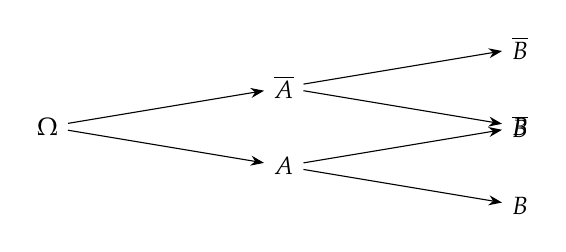
\begin{tikzpicture}[grow=right,level distance=30mm,sibling distance=10mm,every node/.style={font=\small},edge from parent/.style={draw,-{Stealth}}]
\node {$\Omega$} child {node {$A$} child {node {$B$}} child {node {$\overline B$}}} child {node {$\overline A$} child {node {$B$}} child {node {$\overline B$}}};
\end{tikzpicture}\end{center}
    \end{activite}
    \enseignant{$P(D)=0{,}2\times0{,}01+0{,}5\times0{,}02+0{,}3\times0{,}04=0{,}024$, soit $2{,}4\,\%$. Faire verbaliser la donnée qui déclenche le choix de méthode.}

    \begin{traceecrite}Si $(A_i)$ est une partition, $P(B)=\sum_i P(A_i)P_{A_i}(B)$. Chaque terme correspond à un chemin menant à $B$.\end{traceecrite}

    \begin{exemple}
    Reprendre les données de l'activité et rédiger la solution dans l'ordre : définition des objets, propriété utilisée, calcul exact ou approché, puis phrase de réponse. La réponse modèle figure dans l'édition enseignant.
    \end{exemple}
    \enseignant{$P(D)=0{,}2\times0{,}01+0{,}5\times0{,}02+0{,}3\times0{,}04=0{,}024$, soit $2{,}4\,\%$.}

    \begin{exercice}[-- essentiel]
    \begin{enumerate}\item On sait $P(A)=0{,}25$, $P_A(B)=0{,}5$ et $P_{\overline A}(B)=0{,}7$. Construire l'arbre.\item Calculer $P(A\cap B)$ puis $P(B)$.\item Calculer $P_B(A)$ et tester l'indépendance.\end{enumerate}
    \end{exercice}
    \enseignant{$P(A\cap B)=0{,}25\times0{,}5$. Puis $P(B)=P(A)P_A(B)+(1-P(A))P_{\overline A}(B)$ et $P_B(A)=\dfrac{P(A\cap B)}{P(B)}$. Comparer à $P(A)$.}

    \manuelref{Calao, p. 138, n° 1 à 5, puis p. 142, n° 22 à 25}
\ExoSession{43}

    \begin{dm}Reprendre l'exercice d'entraînement 2 avec les données suivantes : remplacer la donnée initiale par $335$ et le taux ou la raison par $3$. Rédiger en quatre lignes : données, formule, calcul, conclusion.\end{dm}
    \enseignant{La correction dépend de l'exercice repris. Vérifier surtout la cohérence du modèle, le nombre d'itérations, l'arrondi et la phrase de conclusion.}

    \begin{sortie}Sur une demi-feuille : écrire la règle principale de la séance, traiter un exemple très court et indiquer son degré de confiance de 1 à 4. Question(s) essentielle(s) du jour : 1, 2 et 3.\end{sortie}

    \ifprof
    \begin{methode}
    \textbf{Conduite en 1 h :} 7 min d'automatismes ; 10 min de mise en commun et trace ; 28 min d'exercices essentiels ; 5 min de correction ; 3 min de billet de sortie.\\
    \textbf{Conduite en 2 h :} ajouter 20 min de recherche de l'activité, 20 min d'institutionnalisation, un second exercice autonome et 10 min de correction comparée.\\
    \textbf{Différenciation :} fournir aux élèves fragiles une fiche à quatre cases (données, modèle, calcul, conclusion). Demander aux élèves rapides de produire un contre-exemple, une justification ou une seconde méthode.
    \end{methode}
    \fi
\sessionheader{44}{25/03/2027}{B : 1 h -- C : 2 h}{Problèmes contextualisés}{Probabilités conditionnelles}
\begin{objectifs}\begin{itemize}\item Choisir arbre ou tableau.\item Résoudre un problème contextualisé.\item Interpréter.\end{itemize}\end{objectifs}
\begin{automatismes}\begin{enumerate}\item Réduire $3x+5-x+2$. \rep{$2x+7$}\item Calculer $0{,}5\times0{,}4$. \rep{$0,20$}\item Si $P(A)=0{,}37$, calculer $P(\overline A)$. \rep{$0{,}63$}\item Simplifier $\dfrac{18}{30}$. \rep{$\dfrac35$}\item Que vaut la somme des branches issues d'un nœud ? \rep{$1$}\end{enumerate}\end{automatismes}
\begin{prerequis}Relire la dernière trace écrite et savoir effectuer les calculs élémentaires mobilisés aujourd'hui. Avant l'activité, faire reformuler les mots-clés : choisir arbre ou tableau et résoudre un problème contextualisé.\end{prerequis}

\begin{activite}
Transformer un tableau d'effectifs clients/abonnement/résiliation en arbre, puis répondre à une question dans chaque sens : probabilité de résilier sachant l'abonnement ; probabilité d'avoir l'abonnement sachant la résiliation.

\end{activite}
\enseignant{La première lecture utilise une ligne ou une branche ; la seconde nécessite de rapporter l'intersection au total des résiliations. Faire verbaliser la donnée qui déclenche le choix de méthode.}

\begin{traceecrite}Choisir entre arbre et tableau : l'arbre met en valeur l'ordre du conditionnement ; le tableau convient bien aux effectifs et aux lectures inversées.\end{traceecrite}

\begin{exemple}
Reprendre les données de l'activité et rédiger la solution dans l'ordre : définition des objets, propriété utilisée, calcul exact ou approché, puis phrase de réponse. La réponse modèle figure dans l'édition enseignant.
\end{exemple}
\enseignant{La première lecture utilise une ligne ou une branche ; la seconde nécessite de rapporter l'intersection au total des résiliations.}

\begin{exercice}[-- essentiel]
\begin{enumerate}\item On sait $P(A)=0{,}30$, $P_A(B)=0{,}6$ et $P_{\overline A}(B)=0{,}8$. Construire l'arbre.\item Calculer $P(A\cap B)$ puis $P(B)$.\item Calculer $P_B(A)$ et tester l'indépendance.\end{enumerate}
\end{exercice}
\enseignant{$P(A\cap B)=0{,}30\times0{,}6$. Puis $P(B)=P(A)P_A(B)+(1-P(A))P_{\overline A}(B)$ et $P_B(A)=\dfrac{P(A\cap B)}{P(B)}$. Comparer à $P(A)$.}

\manuelref{Calao, p. 142, n° 22 à 25, puis p. 144, n° 30 à 32}
\ExoSession{44}

\begin{dm}Reprendre l'exercice d'entraînement 3 avec les données suivantes : remplacer la donnée initiale par $340$ et le taux ou la raison par $4$. Rédiger en quatre lignes : données, formule, calcul, conclusion.\end{dm}
\enseignant{La correction dépend de l'exercice repris. Vérifier surtout la cohérence du modèle, le nombre d'itérations, l'arrondi et la phrase de conclusion.}

\begin{sortie}Sur une demi-feuille : écrire la règle principale de la séance, traiter un exemple très court et indiquer son degré de confiance de 1 à 4. Question(s) essentielle(s) du jour : 1 et 2.\end{sortie}

\ifprof
\begin{methode}
\textbf{Conduite en 1 h :} 7 min d'automatismes ; 10 min de mise en commun et trace ; 28 min d'exercices essentiels ; 5 min de correction ; 3 min de billet de sortie.\\
\textbf{Conduite en 2 h :} ajouter 20 min de recherche de l'activité, 20 min d'institutionnalisation, un second exercice autonome et 10 min de correction comparée.\\
\textbf{Différenciation :} fournir aux élèves fragiles une fiche à quatre cases (données, modèle, calcul, conclusion). Demander aux élèves rapides de produire un contre-exemple, une justification ou une seconde méthode.
\end{methode}
\fi
\sessionheader{45}{30/03/2027}{B : 2 h -- C : 1 h}{Entraînement mixte}{Probabilités conditionnelles}
    \begin{objectifs}\begin{itemize}\item Calculer une probabilité inverse.\item Enchaîner total et conditionnement.\item Contrôler le résultat.\end{itemize}\end{objectifs}
    \begin{automatismes}\begin{enumerate}\item Calculer $20\,\%$ de $120$. \rep{$24$}\item Si $P(A)=0{,}37$, calculer $P(\overline A)$. \rep{$0{,}63$}\item Simplifier $\dfrac{18}{30}$. \rep{$\dfrac35$}\item Que vaut la somme des branches issues d'un nœud ? \rep{$1$}\item Calculer $0{,}6\times0{,}4$. \rep{$0,24$}\end{enumerate}\end{automatismes}
    \begin{prerequis}Relire la dernière trace écrite et savoir effectuer les calculs élémentaires mobilisés aujourd'hui. Avant l'activité, faire reformuler les mots-clés : calculer une probabilité inverse et enchaîner total et conditionnement.\end{prerequis}

    \begin{activite}
    Dans la situation de la séance 43, sachant qu'un article est défectueux, calculer la probabilité qu'il provienne de la ligne C. Expliquer pourquoi ce résultat n'est pas $30\,\%$.
    \begin{center}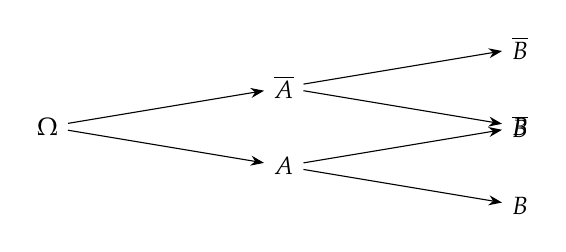
\begin{tikzpicture}[grow=right,level distance=30mm,sibling distance=10mm,every node/.style={font=\small},edge from parent/.style={draw,-{Stealth}}]
\node {$\Omega$} child {node {$A$} child {node {$B$}} child {node {$\overline B$}}} child {node {$\overline A$} child {node {$B$}} child {node {$\overline B$}}};
\end{tikzpicture}\end{center}
    \end{activite}
    \enseignant{$P_D(C)=\dfrac{0{,}3\times0{,}04}{0{,}024}=0{,}5$. Le conditionnement modifie la répartition parce que les taux de défaut diffèrent. Faire verbaliser la donnée qui déclenche le choix de méthode.}

    \begin{traceecrite}Pour une probabilité inverse, calculer d'abord la probabilité totale de l'événement conditionnant, puis utiliser la définition de la probabilité conditionnelle.\end{traceecrite}

    \begin{exemple}
    Reprendre les données de l'activité et rédiger la solution dans l'ordre : définition des objets, propriété utilisée, calcul exact ou approché, puis phrase de réponse. La réponse modèle figure dans l'édition enseignant.
    \end{exemple}
    \enseignant{$P_D(C)=\dfrac{0{,}3\times0{,}04}{0{,}024}=0{,}5$. Le conditionnement modifie la répartition parce que les taux de défaut diffèrent.}

    \begin{exercice}[-- essentiel]
    \begin{enumerate}\item On sait $P(A)=0{,}35$, $P_A(B)=0{,}2$ et $P_{\overline A}(B)=0{,}4$. Construire l'arbre.\item Calculer $P(A\cap B)$ puis $P(B)$.\item Calculer $P_B(A)$ et tester l'indépendance.\end{enumerate}
    \end{exercice}
    \enseignant{$P(A\cap B)=0{,}35\times0{,}2$. Puis $P(B)=P(A)P_A(B)+(1-P(A))P_{\overline A}(B)$ et $P_B(A)=\dfrac{P(A\cap B)}{P(B)}$. Comparer à $P(A)$.}

    \manuelref{Calao, p. 144 à 146}
\ExoSession{45}

    \begin{dm}Reprendre l'exercice d'entraînement 2 avec les données suivantes : remplacer la donnée initiale par $345$ et le taux ou la raison par $5$. Rédiger en quatre lignes : données, formule, calcul, conclusion.\end{dm}
    \enseignant{La correction dépend de l'exercice repris. Vérifier surtout la cohérence du modèle, le nombre d'itérations, l'arrondi et la phrase de conclusion.}

    \begin{sortie}Sur une demi-feuille : écrire la règle principale de la séance, traiter un exemple très court et indiquer son degré de confiance de 1 à 4. Question(s) essentielle(s) du jour : 1, 2 et 3.\end{sortie}

    \ifprof
    \begin{methode}
    \textbf{Conduite en 1 h :} 7 min d'automatismes ; 10 min de mise en commun et trace ; 28 min d'exercices essentiels ; 5 min de correction ; 3 min de billet de sortie.\\
    \textbf{Conduite en 2 h :} ajouter 20 min de recherche de l'activité, 20 min d'institutionnalisation, un second exercice autonome et 10 min de correction comparée.\\
    \textbf{Différenciation :} fournir aux élèves fragiles une fiche à quatre cases (données, modèle, calcul, conclusion). Demander aux élèves rapides de produire un contre-exemple, une justification ou une seconde méthode.
    \end{methode}
    \fi
\sessionheader{46}{01/04/2027}{B : 1 h -- C : 2 h}{Bilan et évaluation}{Probabilités conditionnelles}
\begin{objectifs}\begin{itemize}\item Mobiliser toutes les méthodes.\item Rédiger avec les notations.\item Remédier aux erreurs.\end{itemize}\end{objectifs}
\begin{automatismes}\begin{enumerate}\item Écrire le coefficient multiplicateur d'une hausse de $25\,\%$. \rep{$1+\dfrac{25}{100}=1,25$}\item Simplifier $\dfrac{18}{30}$. \rep{$\dfrac35$}\item Que vaut la somme des branches issues d'un nœud ? \rep{$1$}\item Calculer $0{,}7\times0{,}4$. \rep{$0,28$}\item Si $P(A)=0{,}37$, calculer $P(\overline A)$. \rep{$0{,}63$}\end{enumerate}\end{automatismes}
\begin{prerequis}Relire la dernière trace écrite et savoir effectuer les calculs élémentaires mobilisés aujourd'hui. Avant l'activité, faire reformuler les mots-clés : mobiliser toutes les méthodes et rédiger avec les notations.\end{prerequis}

\begin{activite}
Réaliser un parcours de quatre postes : compléter un arbre ; calculer une intersection ; appliquer la formule totale ; tester l'indépendance. Chaque groupe laisse une justification écrite au groupe suivant.

\end{activite}
\enseignant{Les productions doivent contenir formules et interprétations. Les erreurs sont classées : notation, complément, produit, somme, conditionnement inverse. Faire verbaliser la donnée qui déclenche le choix de méthode.}

\begin{traceecrite}Toujours nommer les événements, compléter toutes les branches, écrire la formule avant le calcul et interpréter la probabilité finale.\end{traceecrite}

\begin{exemple}
Reprendre les données de l'activité et rédiger la solution dans l'ordre : définition des objets, propriété utilisée, calcul exact ou approché, puis phrase de réponse. La réponse modèle figure dans l'édition enseignant.
\end{exemple}
\enseignant{Les productions doivent contenir formules et interprétations. Les erreurs sont classées : notation, complément, produit, somme, conditionnement inverse.}

\begin{exercice}[-- essentiel]
\begin{enumerate}\item On sait $P(A)=0{,}40$, $P_A(B)=0{,}3$ et $P_{\overline A}(B)=0{,}5$. Construire l'arbre.\item Calculer $P(A\cap B)$ puis $P(B)$.\item Calculer $P_B(A)$ et tester l'indépendance.\end{enumerate}
\end{exercice}
\enseignant{$P(A\cap B)=0{,}40\times0{,}3$. Puis $P(B)=P(A)P_A(B)+(1-P(A))P_{\overline A}(B)$ et $P_B(A)=\dfrac{P(A\cap B)}{P(B)}$. Comparer à $P(A)$.}

\manuelref{Calao, p. 146--147}
\ExoSession{46}

\begin{dm}Reprendre l'exercice d'entraînement 3 avec les données suivantes : remplacer la donnée initiale par $350$ et le taux ou la raison par $6$. Rédiger en quatre lignes : données, formule, calcul, conclusion.\end{dm}
\enseignant{La correction dépend de l'exercice repris. Vérifier surtout la cohérence du modèle, le nombre d'itérations, l'arrondi et la phrase de conclusion.}

\begin{sortie}Sur une demi-feuille : écrire la règle principale de la séance, traiter un exemple très court et indiquer son degré de confiance de 1 à 4. Question(s) essentielle(s) du jour : 1 et 2.\end{sortie}

\ifprof
\begin{methode}
\textbf{Conduite en 1 h :} 7 min d'automatismes ; 10 min de mise en commun et trace ; 28 min d'exercices essentiels ; 5 min de correction ; 3 min de billet de sortie.\\
\textbf{Conduite en 2 h :} ajouter 20 min de recherche de l'activité, 20 min d'institutionnalisation, un second exercice autonome et 10 min de correction comparée.\\
\textbf{Différenciation :} fournir aux élèves fragiles une fiche à quatre cases (données, modèle, calcul, conclusion). Demander aux élèves rapides de produire un contre-exemple, une justification ou une seconde méthode.
\end{methode}
\fi


\chapter{Variables aléatoires discrètes et loi binomiale}
\competences{définir une loi, calculer et interpréter une espérance, reconnaître et utiliser une loi binomiale}
\section{Cours de référence}
Une variable aléatoire discrète $X$ associe un nombre réel à chaque issue. Sa loi donne les valeurs $x_i$ et les probabilités $p_i=P(X=x_i)$, avec $p_i\geq0$ et $\sum p_i=1$.

\begin{retenir}
L'espérance est $E(X)=\sum_i x_ip_i$. Elle représente la valeur moyenne à long terme lorsque l'expérience est répétée dans les mêmes conditions ; elle n'est pas nécessairement une valeur effectivement prise par $X$.
\end{retenir}

\begin{center}
\begin{tikzpicture}[node distance=9mm and 16mm,every node/.style={draw,circle,inner sep=1.5pt,font=\small}]
\node (a) {1};
\node[below left=of a] (b) {1}; \node[below right=of a] (c) {1};
\node[below left=of b] (d) {1}; \node[below=of a] (e) {2}; \node[below right=of c] (f) {1};
\node[below left=of d] (g) {1}; \node[below left=of e] (h) {3}; \node[below right=of e] (i) {3}; \node[below right=of f] (j) {1};
\draw (a)--(b) (a)--(c) (b)--(d) (b)--(e) (c)--(e) (c)--(f) (d)--(g) (d)--(h) (e)--(h) (e)--(i) (f)--(i) (f)--(j);
\end{tikzpicture}
\end{center}

\begin{retenir}
$X$ suit une loi binomiale $\mathcal B(n,p)$ lorsque $X$ compte le nombre de succès dans $n$ épreuves de Bernoulli indépendantes, de même probabilité de succès $p$. Alors
\[
P(X=k)=\binom nk p^k(1-p)^{n-k},\qquad E(X)=np.
\]
\end{retenir}

Le coefficient $\binom nk$ compte le nombre de chemins contenant exactement $k$ succès parmi $n$ épreuves. Pour $n\leq10$, il peut être lu dans le triangle de Pascal.

\begin{center}
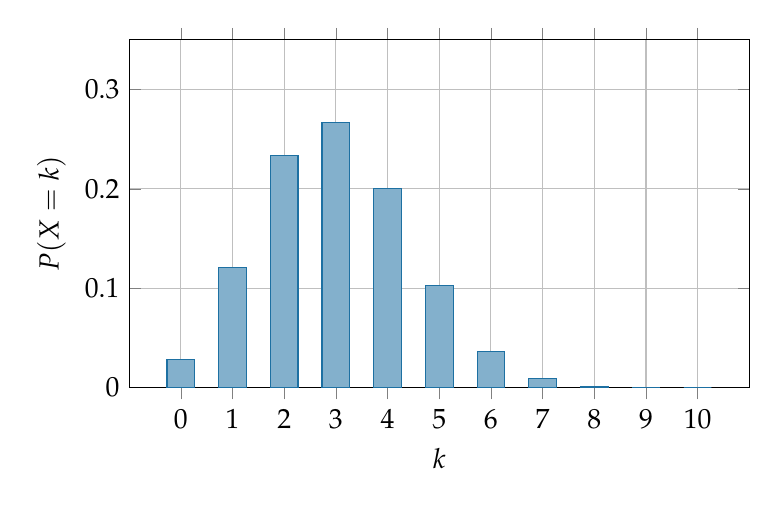
\begin{tikzpicture}
\begin{axis}[ybar,width=.78\textwidth,height=6cm,xlabel={$k$},ylabel={$P(X=k)$},ymin=0,ymax=.35,xtick=data,grid=major]
\addplot[fill=Blue!55,draw=Blue] coordinates {(0,.0282)(1,.1211)(2,.2335)(3,.2668)(4,.2001)(5,.1029)(6,.0368)(7,.0090)(8,.0015)(9,.0002)(10,.0000)};
\end{axis}
\end{tikzpicture}
\end{center}
Le diagramme représente approximativement $\mathcal B(10,0{,}3)$ ; son centre est proche de $E(X)=3$.

\sessionheader{47}{06/04/2027}{B : 2 h -- C : 1 h}{Espérance d'une variable aléatoire}{Variables aléatoires discrètes}
\begin{objectifs}\begin{itemize}\item Définir une loi.\item Calculer une espérance.\item Interpréter une moyenne théorique.\end{itemize}\end{objectifs}
\begin{automatismes}\begin{enumerate}\item Réduire $3x+8-x+2$. \rep{$2x+10$}\item Donner $E(X)$ pour $X\sim\mathcal B(10,0{,}3)$. \rep{$3$}\item Calculer $\binom52$. \rep{$10$}\item Calculer l'espérance de $X$ constant égal à $8$. \rep{$8$}\item Traduire $X\geq1$ par un complémentaire. \rep{$1-P(X=0)$}\end{enumerate}\end{automatismes}
\begin{prerequis}Relire la dernière trace écrite et savoir effectuer les calculs élémentaires mobilisés aujourd'hui. Avant l'activité, faire reformuler les mots-clés : définir une loi et calculer une espérance.\end{prerequis}

\begin{activite}
Un jeu coûte $2$ euros. Le gain brut vaut $0$, $3$ ou $10$ euros avec probabilités $0{,}6$, $0{,}3$, $0{,}1$. Construire la loi du gain net $X$, calculer $E(X)$ et décider si le jeu est favorable au joueur.

\end{activite}
\enseignant{$X$ vaut $-2,1,8$. $E(X)=-1{,}2+0{,}3+0{,}8=-0{,}1$ euro : jeu défavorable en moyenne. Faire verbaliser la donnée qui déclenche le choix de méthode.}

\begin{traceecrite}La loi de $X$ associe à chaque valeur $x_i$ la probabilité $p_i$. L'espérance $E(X)=\sum x_ip_i$ est une moyenne théorique à long terme.\end{traceecrite}

\begin{exemple}
Reprendre les données de l'activité et rédiger la solution dans l'ordre : définition des objets, propriété utilisée, calcul exact ou approché, puis phrase de réponse. La réponse modèle figure dans l'édition enseignant.
\end{exemple}
\enseignant{$X$ vaut $-2,1,8$. $E(X)=-1{,}2+0{,}3+0{,}8=-0{,}1$ euro : jeu défavorable en moyenne.}

\begin{exercice}[-- essentiel]
\begin{enumerate}\item Justifier que le nombre de succès parmi $8$ essais indépendants, avec $p=0{,}3$, suit une loi binomiale.\item Calculer $P(X=2)$ et $P(X=0)$.\item En déduire $P(X\geq1)$ et calculer $E(X)$.\end{enumerate}
\end{exercice}
\enseignant{$X\sim\mathcal B(8,0{,}3)$. $P(X=2)=\binom{8}2 0{,}3^2 0{,}7^{6}$, $P(X=0)=0{,}7^{8}$, $P(X\geq1)=1-P(X=0)$ et $E(X)=\dfrac{24}{10}$.}

\manuelref{Calao, cours p. 154--159 ; exercices p. 160, n° 1 à 5}
\CalaoSession{47}

\begin{dm}Reprendre l'exercice d'entraînement 2 avec les données suivantes : remplacer la donnée initiale par $355$ et le taux ou la raison par $7$. Rédiger en quatre lignes : données, formule, calcul, conclusion.\end{dm}
\enseignant{La correction dépend de l'exercice repris. Vérifier surtout la cohérence du modèle, le nombre d'itérations, l'arrondi et la phrase de conclusion.}

\begin{sortie}Sur une demi-feuille : écrire la règle principale de la séance, traiter un exemple très court et indiquer son degré de confiance de 1 à 4. Question(s) essentielle(s) du jour : 1, 2 et 3.\end{sortie}

\ifprof
\begin{methode}
\textbf{Conduite en 1 h :} 7 min d'automatismes ; 10 min de mise en commun et trace ; 28 min d'exercices essentiels ; 5 min de correction ; 3 min de billet de sortie.\\
\textbf{Conduite en 2 h :} ajouter 20 min de recherche de l'activité, 20 min d'institutionnalisation, un second exercice autonome et 10 min de correction comparée.\\
\textbf{Différenciation :} fournir aux élèves fragiles une fiche à quatre cases (données, modèle, calcul, conclusion). Demander aux élèves rapides de produire un contre-exemple, une justification ou une seconde méthode.
\end{methode}
\fi
\sessionheader{48}{08/04/2027}{B : 1 h -- C : 2 h}{Loi binomiale : reconnaître une situation}{Variables aléatoires discrètes}
\begin{objectifs}\begin{itemize}\item Reconnaître un schéma de Bernoulli.\item Identifier $n$ et $p$.\item Définir $X$.\end{itemize}\end{objectifs}
\begin{automatismes}\begin{enumerate}\item Calculer $5\,\%$ de $180$. \rep{$9$}\item Calculer $\binom52$. \rep{$10$}\item Calculer l'espérance de $X$ constant égal à $9$. \rep{$9$}\item Traduire $X\geq1$ par un complémentaire. \rep{$1-P(X=0)$}\item Donner $E(X)$ pour $X\sim\mathcal B(10,0{,}3)$. \rep{$3$}\end{enumerate}\end{automatismes}
\begin{prerequis}Relire la dernière trace écrite et savoir effectuer les calculs élémentaires mobilisés aujourd'hui. Avant l'activité, faire reformuler les mots-clés : reconnaître un schéma de bernoulli et identifier $n$ et $p$.\end{prerequis}

\begin{activite}
Un client accepte une offre avec probabilité $0{,}25$. Un conseiller contacte indépendamment huit clients. Définir $X$, justifier la loi binomiale et identifier $n$ et $p$.

\end{activite}
\enseignant{$X$ compte les acceptations ; répétition de 8 épreuves identiques et indépendantes, succès de probabilité $0{,}25$ : $X\sim\mathcal B(8,0{,}25)$. Faire verbaliser la donnée qui déclenche le choix de méthode.}

\begin{traceecrite}$X\sim\mathcal B(n,p)$ si $X$ compte les succès dans $n$ épreuves indépendantes de même probabilité $p$.\end{traceecrite}

\begin{exemple}
Reprendre les données de l'activité et rédiger la solution dans l'ordre : définition des objets, propriété utilisée, calcul exact ou approché, puis phrase de réponse. La réponse modèle figure dans l'édition enseignant.
\end{exemple}
\enseignant{$X$ compte les acceptations ; répétition de 8 épreuves identiques et indépendantes, succès de probabilité $0{,}25$ : $X\sim\mathcal B(8,0{,}25)$.}

\begin{exercice}[-- essentiel]
\begin{enumerate}\item Justifier que le nombre de succès parmi $9$ essais indépendants, avec $p=0{,}3$, suit une loi binomiale.\item Calculer $P(X=2)$ et $P(X=0)$.\item En déduire $P(X\geq1)$ et calculer $E(X)$.\end{enumerate}
\end{exercice}
\enseignant{$X\sim\mathcal B(9,0{,}3)$. $P(X=2)=\binom{9}2 0{,}3^2 0{,}7^{7}$, $P(X=0)=0{,}7^{9}$, $P(X\geq1)=1-P(X=0)$ et $E(X)=\dfrac{27}{10}$.}

\manuelref{Calao, cours p. 154--159 ; exercices p. 160, n° 5, puis p. 162, n° 14 à 20}
\CalaoSession{48}

\begin{dm}Reprendre l'exercice d'entraînement 3 avec les données suivantes : remplacer la donnée initiale par $360$ et le taux ou la raison par $2$. Rédiger en quatre lignes : données, formule, calcul, conclusion.\end{dm}
\enseignant{La correction dépend de l'exercice repris. Vérifier surtout la cohérence du modèle, le nombre d'itérations, l'arrondi et la phrase de conclusion.}

\begin{sortie}Sur une demi-feuille : écrire la règle principale de la séance, traiter un exemple très court et indiquer son degré de confiance de 1 à 4. Question(s) essentielle(s) du jour : 1 et 2.\end{sortie}

\ifprof
\begin{methode}
\textbf{Conduite en 1 h :} 7 min d'automatismes ; 10 min de mise en commun et trace ; 28 min d'exercices essentiels ; 5 min de correction ; 3 min de billet de sortie.\\
\textbf{Conduite en 2 h :} ajouter 20 min de recherche de l'activité, 20 min d'institutionnalisation, un second exercice autonome et 10 min de correction comparée.\\
\textbf{Différenciation :} fournir aux élèves fragiles une fiche à quatre cases (données, modèle, calcul, conclusion). Demander aux élèves rapides de produire un contre-exemple, une justification ou une seconde méthode.
\end{methode}
\fi
\sessionheader{49}{27/04/2027}{B : 2 h -- C : 1 h}{Triangle de Pascal et coefficients binomiaux}{Variables aléatoires discrètes}
\begin{objectifs}\begin{itemize}\item Construire le triangle de Pascal.\item Lire $\binom nk$.\item Interpréter un coefficient.\end{itemize}\end{objectifs}
\begin{automatismes}\begin{enumerate}\item Écrire le coefficient multiplicateur d'une hausse de $10\,\%$. \rep{$1+\dfrac{10}{100}=1,10$}\item Calculer l'espérance de $X$ constant égal à $3$. \rep{$3$}\item Traduire $X\geq1$ par un complémentaire. \rep{$1-P(X=0)$}\item Donner $E(X)$ pour $X\sim\mathcal B(10,0{,}3)$. \rep{$3$}\item Calculer $\binom52$. \rep{$10$}\end{enumerate}\end{automatismes}
\begin{prerequis}Relire la dernière trace écrite et savoir effectuer les calculs élémentaires mobilisés aujourd'hui. Avant l'activité, faire reformuler les mots-clés : construire le triangle de pascal et lire $\binom nk$.\end{prerequis}

\begin{activite}
Construire les lignes $n=0$ à $n=6$ du triangle de Pascal. Expliquer le calcul du nombre $15$ de la ligne $6$, puis lire $\binom62$ et $\binom64$.
\begin{center}\begin{tabular}{*{9}{c}}&&&&1&&&&\\&&&1&&1&&&\\&&1&&2&&1&&\\&1&&3&&3&&1&\\1&&4&&6&&4&&1\end{tabular}\end{center}
\end{activite}
\enseignant{Chaque nombre intérieur est la somme des deux nombres situés au-dessus. $\binom62=\binom64=15$. Faire verbaliser la donnée qui déclenche le choix de méthode.}

\begin{traceecrite}Le triangle de Pascal vérifie $\binom nk=\binom{n-1}{k-1}+\binom{n-1}{k}$. Les bords valent $1$.\end{traceecrite}

\begin{exemple}
Reprendre les données de l'activité et rédiger la solution dans l'ordre : définition des objets, propriété utilisée, calcul exact ou approché, puis phrase de réponse. La réponse modèle figure dans l'édition enseignant.
\end{exemple}
\enseignant{Chaque nombre intérieur est la somme des deux nombres situés au-dessus. $\binom62=\binom64=15$.}

\begin{exercice}[-- essentiel]
\begin{enumerate}\item Justifier que le nombre de succès parmi $10$ essais indépendants, avec $p=0{,}3$, suit une loi binomiale.\item Calculer $P(X=2)$ et $P(X=0)$.\item En déduire $P(X\geq1)$ et calculer $E(X)$.\end{enumerate}
\end{exercice}
\enseignant{$X\sim\mathcal B(10,0{,}3)$. $P(X=2)=\binom{10}2 0{,}3^2 0{,}7^{8}$, $P(X=0)=0{,}7^{10}$, $P(X\geq1)=1-P(X=0)$ et $E(X)=\dfrac{30}{10}$.}

\manuelref{Calao, p. 164, n° 24 à 29, puis p. 166, n° 36}
\CalaoSession{49}

\begin{dm}Reprendre l'exercice d'entraînement 2 avec les données suivantes : remplacer la donnée initiale par $365$ et le taux ou la raison par $3$. Rédiger en quatre lignes : données, formule, calcul, conclusion.\end{dm}
\enseignant{La correction dépend de l'exercice repris. Vérifier surtout la cohérence du modèle, le nombre d'itérations, l'arrondi et la phrase de conclusion.}

\begin{sortie}Sur une demi-feuille : écrire la règle principale de la séance, traiter un exemple très court et indiquer son degré de confiance de 1 à 4. Question(s) essentielle(s) du jour : 1, 2 et 3.\end{sortie}

\ifprof
\begin{methode}
\textbf{Conduite en 1 h :} 7 min d'automatismes ; 10 min de mise en commun et trace ; 28 min d'exercices essentiels ; 5 min de correction ; 3 min de billet de sortie.\\
\textbf{Conduite en 2 h :} ajouter 20 min de recherche de l'activité, 20 min d'institutionnalisation, un second exercice autonome et 10 min de correction comparée.\\
\textbf{Différenciation :} fournir aux élèves fragiles une fiche à quatre cases (données, modèle, calcul, conclusion). Demander aux élèves rapides de produire un contre-exemple, une justification ou une seconde méthode.
\end{methode}
\fi
\sessionheader{50}{29/04/2027}{B : 1 h -- C : 2 h}{Probabilités binomiales}{Variables aléatoires discrètes}
\begin{objectifs}\begin{itemize}\item Calculer $P(X=k)$.\item Traduire au moins/au plus.\item Utiliser le complémentaire.\end{itemize}\end{objectifs}
\begin{automatismes}\begin{enumerate}\item Réduire $3x+4-x+2$. \rep{$2x+6$}\item Traduire $X\geq1$ par un complémentaire. \rep{$1-P(X=0)$}\item Donner $E(X)$ pour $X\sim\mathcal B(10,0{,}3)$. \rep{$3$}\item Calculer $\binom52$. \rep{$10$}\item Calculer l'espérance de $X$ constant égal à $4$. \rep{$4$}\end{enumerate}\end{automatismes}
\begin{prerequis}Relire la dernière trace écrite et savoir effectuer les calculs élémentaires mobilisés aujourd'hui. Avant l'activité, faire reformuler les mots-clés : calculer $p(x=k)$ et traduire au moins/au plus.\end{prerequis}

\begin{activite}
Pour $X\sim\mathcal B(8,0{,}25)$, calculer $P(X=2)$, $P(X=0)$ puis $P(X\geq1)$. Traduire chaque événement en phrase.
\begin{center}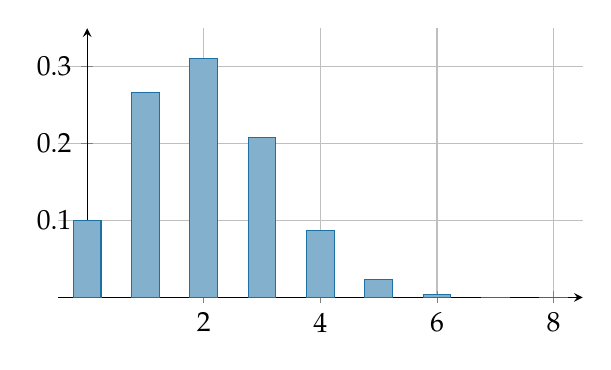
\begin{tikzpicture}\begin{axis}[width=.68\textwidth,height=5cm,axis lines=middle,xmin=-.5,xmax=8.5,ymin=0,ymax=.35,grid=major]\addplot[ybar,fill=Blue!55,draw=Blue] coordinates {(0,.10)(1,.267)(2,.311)(3,.208)(4,.087)(5,.023)(6,.004)(7,.0004)(8,.00002)};\end{axis}\end{tikzpicture}\end{center}
\end{activite}
\enseignant{$P(X=2)=\binom82 0{,}25^2 0{,}75^6\approx0{,}3115$ ; $P(X=0)=0{,}75^8\approx0{,}1001$ ; $P(X\geq1)\approx0{,}8999$. Faire verbaliser la donnée qui déclenche le choix de méthode.}

\begin{traceecrite}Si $X\sim\mathcal B(n,p)$, alors $P(X=k)=\binom nkp^k(1-p)^{n-k}$. Traduire soigneusement « au moins », « au plus » et « aucun ».\end{traceecrite}

\begin{exemple}
Reprendre les données de l'activité et rédiger la solution dans l'ordre : définition des objets, propriété utilisée, calcul exact ou approché, puis phrase de réponse. La réponse modèle figure dans l'édition enseignant.
\end{exemple}
\enseignant{$P(X=2)=\binom82 0{,}25^2 0{,}75^6\approx0{,}3115$ ; $P(X=0)=0{,}75^8\approx0{,}1001$ ; $P(X\geq1)\approx0{,}8999$.}

\begin{exercice}[-- essentiel]
\begin{enumerate}\item Justifier que le nombre de succès parmi $6$ essais indépendants, avec $p=0{,}3$, suit une loi binomiale.\item Calculer $P(X=2)$ et $P(X=0)$.\item En déduire $P(X\geq1)$ et calculer $E(X)$.\end{enumerate}
\end{exercice}
\enseignant{$X\sim\mathcal B(6,0{,}3)$. $P(X=2)=\binom{6}2 0{,}3^2 0{,}7^{4}$, $P(X=0)=0{,}7^{6}$, $P(X\geq1)=1-P(X=0)$ et $E(X)=\dfrac{18}{10}$.}

\manuelref{Calao, p. 164, n° 24 à 29, puis p. 168, n° 41 à 45}
\CalaoSession{50}

\begin{dm}Reprendre l'exercice d'entraînement 3 avec les données suivantes : remplacer la donnée initiale par $370$ et le taux ou la raison par $4$. Rédiger en quatre lignes : données, formule, calcul, conclusion.\end{dm}
\enseignant{La correction dépend de l'exercice repris. Vérifier surtout la cohérence du modèle, le nombre d'itérations, l'arrondi et la phrase de conclusion.}

\begin{sortie}Sur une demi-feuille : écrire la règle principale de la séance, traiter un exemple très court et indiquer son degré de confiance de 1 à 4. Question(s) essentielle(s) du jour : 1 et 2.\end{sortie}

\ifprof
\begin{methode}
\textbf{Conduite en 1 h :} 7 min d'automatismes ; 10 min de mise en commun et trace ; 28 min d'exercices essentiels ; 5 min de correction ; 3 min de billet de sortie.\\
\textbf{Conduite en 2 h :} ajouter 20 min de recherche de l'activité, 20 min d'institutionnalisation, un second exercice autonome et 10 min de correction comparée.\\
\textbf{Différenciation :} fournir aux élèves fragiles une fiche à quatre cases (données, modèle, calcul, conclusion). Demander aux élèves rapides de produire un contre-exemple, une justification ou une seconde méthode.
\end{methode}
\fi
\sessionheader{51}{04/05/2027}{B : 2 h -- C : 1 h}{Bilan du chapitre et évaluation}{Variables aléatoires discrètes}
\begin{objectifs}\begin{itemize}\item Calculer et interpréter $E(X)$.\item Résoudre un problème binomial.\item Analyser ses erreurs.\end{itemize}\end{objectifs}
\begin{automatismes}\begin{enumerate}\item Calculer $20\,\%$ de $100$. \rep{$20$}\item Donner $E(X)$ pour $X\sim\mathcal B(10,0{,}3)$. \rep{$3$}\item Calculer $\binom52$. \rep{$10$}\item Calculer l'espérance de $X$ constant égal à $5$. \rep{$5$}\item Traduire $X\geq1$ par un complémentaire. \rep{$1-P(X=0)$}\end{enumerate}\end{automatismes}
\begin{prerequis}Relire la dernière trace écrite et savoir effectuer les calculs élémentaires mobilisés aujourd'hui. Avant l'activité, faire reformuler les mots-clés : calculer et interpréter $e(x)$ et résoudre un problème binomial.\end{prerequis}

\begin{activite}
Un centre reçoit $120$ groupes de $10$ clients, chaque client réclamant avec probabilité $0{,}08$. Estimer le nombre moyen de réclamations par groupe, puis sur l'ensemble des groupes. Discuter ce que l'espérance permet ou non de prévoir.

\end{activite}
\enseignant{Par groupe $E(X)=10\times0{,}08=0{,}8$. Sur 120 groupes, environ $96$ réclamations en moyenne ; ce n'est pas une certitude. Faire verbaliser la donnée qui déclenche le choix de méthode.}

\begin{traceecrite}Pour $X\sim\mathcal B(n,p)$, $E(X)=np$. La valeur donne le nombre moyen de succès sur un grand nombre de séries de $n$ épreuves.\end{traceecrite}

\begin{exemple}
Reprendre les données de l'activité et rédiger la solution dans l'ordre : définition des objets, propriété utilisée, calcul exact ou approché, puis phrase de réponse. La réponse modèle figure dans l'édition enseignant.
\end{exemple}
\enseignant{Par groupe $E(X)=10\times0{,}08=0{,}8$. Sur 120 groupes, environ $96$ réclamations en moyenne ; ce n'est pas une certitude.}

\begin{exercice}[-- essentiel]
\begin{enumerate}\item Justifier que le nombre de succès parmi $7$ essais indépendants, avec $p=0{,}3$, suit une loi binomiale.\item Calculer $P(X=2)$ et $P(X=0)$.\item En déduire $P(X\geq1)$ et calculer $E(X)$.\end{enumerate}
\end{exercice}
\enseignant{$X\sim\mathcal B(7,0{,}3)$. $P(X=2)=\binom{7}2 0{,}3^2 0{,}7^{5}$, $P(X=0)=0{,}7^{7}$, $P(X\geq1)=1-P(X=0)$ et $E(X)=\dfrac{21}{10}$.}

\manuelref{Calao, p. 160 à 169}
\CalaoSession{51}

\begin{dm}Reprendre l'exercice d'entraînement 2 avec les données suivantes : remplacer la donnée initiale par $375$ et le taux ou la raison par $5$. Rédiger en quatre lignes : données, formule, calcul, conclusion.\end{dm}
\enseignant{La correction dépend de l'exercice repris. Vérifier surtout la cohérence du modèle, le nombre d'itérations, l'arrondi et la phrase de conclusion.}

\begin{sortie}Sur une demi-feuille : écrire la règle principale de la séance, traiter un exemple très court et indiquer son degré de confiance de 1 à 4. Question(s) essentielle(s) du jour : 1, 2 et 3.\end{sortie}

\ifprof
\begin{methode}
\textbf{Conduite en 1 h :} 7 min d'automatismes ; 10 min de mise en commun et trace ; 28 min d'exercices essentiels ; 5 min de correction ; 3 min de billet de sortie.\\
\textbf{Conduite en 2 h :} ajouter 20 min de recherche de l'activité, 20 min d'institutionnalisation, un second exercice autonome et 10 min de correction comparée.\\
\textbf{Différenciation :} fournir aux élèves fragiles une fiche à quatre cases (données, modèle, calcul, conclusion). Demander aux élèves rapides de produire un contre-exemple, une justification ou une seconde méthode.
\end{methode}
\fi


\chapter{Révisions et consolidation}
\section{Stratégie de révision}
\begin{retenir}
Une révision efficace alterne récupération en mémoire, correction explicite des erreurs et réemploi dans un problème. Relire passivement le cours ne suffit pas : il faut tenter une question sans modèle, comparer sa réponse, puis refaire la question après un délai.
\end{retenir}

Pour chaque chapitre, utiliser le code suivant : \textbf{V} (maîtrisé), \textbf{O} (fragile), \textbf{R} (à reprendre). Après le diagnostic, travailler en priorité une compétence orange ou rouge, puis vérifier immédiatement avec une question analogue.

\begin{center}
\begin{tabularx}{.9\textwidth}{lcccX}
\toprule
Compétence & V & O & R & Action de remédiation \\
\midrule
Choisir un modèle & $\square$ & $\square$ & $\square$ & Refaire un exercice de tri arithmétique/géométrique/exponentiel.\\
Lire et calculer & $\square$ & $\square$ & $\square$ & Reprendre les automatismes ciblés.\\
Rédiger et interpréter & $\square$ & $\square$ & $\square$ & Ajouter données, formule, calcul, unité et phrase de réponse.\\
\bottomrule
\end{tabularx}
\end{center}

\sessionheader{52}{11/05/2027}{B : 2 h -- C : 1 h}{Diagnostic des acquis}{Révisions et consolidation}
\begin{objectifs}\begin{itemize}\item Identifier les acquis.\item Classer les erreurs.\item Planifier la remédiation.\end{itemize}\end{objectifs}
\begin{automatismes}\begin{enumerate}\item Écrire le coefficient multiplicateur d'une hausse de $25\,\%$. \rep{$1+\dfrac{25}{100}=1,25$}\item Donner la formule du terme général arithmétique depuis $u_0$. \rep{$u_n=u_0+nr$}\item Résoudre $10^x=1000$. \rep{$x=3$}\item Dériver $x+\dfrac4x$. \rep{$1-\dfrac4{x^2}$}\item Énoncer la formule des probabilités totales avec deux branches. \rep{$P(B)=P(A)P_A(B)+P(\overline A)P_{\overline A}(B)$}\end{enumerate}\end{automatismes}
\begin{prerequis}Relire la dernière trace écrite et savoir effectuer les calculs élémentaires mobilisés aujourd'hui. Avant l'activité, faire reformuler les mots-clés : identifier les acquis et classer les erreurs.\end{prerequis}

\begin{activite}
Répondre sans cours à 14 questions, deux par chapitre. Reporter chaque erreur dans une grille : connaissance, choix de méthode, calcul, lecture, rédaction. Choisir ensuite deux priorités personnelles.

\end{activite}
\enseignant{La correction attend un profil d'erreurs et un plan de reprise, pas seulement une note globale. Faire verbaliser la donnée qui déclenche le choix de méthode.}

\begin{traceecrite}Le diagnostic sert à choisir la remédiation : reconnaître l'erreur, retrouver la règle utile, refaire une question analogue, puis vérifier sans aide.\end{traceecrite}

\begin{exemple}
Reprendre les données de l'activité et rédiger la solution dans l'ordre : définition des objets, propriété utilisée, calcul exact ou approché, puis phrase de réponse. La réponse modèle figure dans l'édition enseignant.
\end{exemple}
\enseignant{La correction attend un profil d'erreurs et un plan de reprise, pas seulement une note globale.}

\begin{exercice}[-- essentiel]
\begin{enumerate}\item Choisir entre suite arithmétique, suite géométrique et fonction exponentielle dans trois situations.\item Résoudre une équation exponentielle avec un logarithme.\item Calculer une probabilité à partir d'un arbre puis interpréter.\end{enumerate}
\end{exercice}
\enseignant{Justifier chaque choix par variation absolue ou relative ; vérifier la positivité avant le logarithme ; multiplier le long d'un chemin et conclure par une phrase.}

\manuelref{Réactivation des chapitres 1 à 7}
\ExoSession{52}

\begin{dm}Reprendre l'exercice d'entraînement 3 avec les données suivantes : remplacer la donnée initiale par $380$ et le taux ou la raison par $6$. Rédiger en quatre lignes : données, formule, calcul, conclusion.\end{dm}
\enseignant{La correction dépend de l'exercice repris. Vérifier surtout la cohérence du modèle, le nombre d'itérations, l'arrondi et la phrase de conclusion.}

\begin{sortie}Sur une demi-feuille : écrire la règle principale de la séance, traiter un exemple très court et indiquer son degré de confiance de 1 à 4. Question(s) essentielle(s) du jour : 1 et 2.\end{sortie}

\ifprof
\begin{methode}
\textbf{Conduite en 1 h :} 7 min d'automatismes ; 10 min de mise en commun et trace ; 28 min d'exercices essentiels ; 5 min de correction ; 3 min de billet de sortie.\\
\textbf{Conduite en 2 h :} ajouter 20 min de recherche de l'activité, 20 min d'institutionnalisation, un second exercice autonome et 10 min de correction comparée.\\
\textbf{Différenciation :} fournir aux élèves fragiles une fiche à quatre cases (données, modèle, calcul, conclusion). Demander aux élèves rapides de produire un contre-exemple, une justification ou une seconde méthode.
\end{methode}
\fi
\sessionheader{53}{13/05/2027}{B : 1 h -- C : 2 h}{Réactivation : fonctions exponentielles}{Révisions et consolidation}
\begin{objectifs}\begin{itemize}\item Réactiver les modèles exponentiels.\item Résoudre et interpréter.\item Contrôler les unités.\end{itemize}\end{objectifs}
\begin{automatismes}\begin{enumerate}\item Réduire $3x+7-x+2$. \rep{$2x+9$}\item Résoudre $10^x=1000$. \rep{$x=3$}\item Dériver $x+\dfrac4x$. \rep{$1-\dfrac4{x^2}$}\item Énoncer la formule des probabilités totales avec deux branches. \rep{$P(B)=P(A)P_A(B)+P(\overline A)P_{\overline A}(B)$}\item Donner la formule du terme général arithmétique depuis $u_0$. \rep{$u_n=u_0+nr$}\end{enumerate}\end{automatismes}
\begin{prerequis}Relire la dernière trace écrite et savoir effectuer les calculs élémentaires mobilisés aujourd'hui. Avant l'activité, faire reformuler les mots-clés : réactiver les modèles exponentiels et résoudre et interpréter.\end{prerequis}

\begin{activite}
Une valeur de $18\,000$ augmente de $3{,}5\,\%$ par an. Écrire le modèle, calculer la valeur après huit ans et déterminer quand elle dépassera $25\,000$.
\begin{center}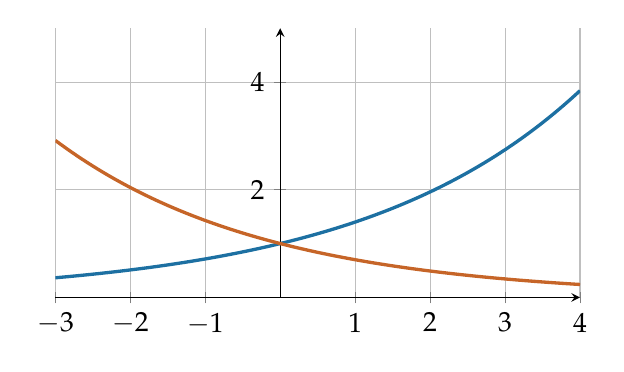
\begin{tikzpicture}\begin{axis}[width=.68\textwidth,height=5cm,axis lines=middle,xmin=-3,xmax=4,ymin=0,ymax=5,grid=major]\addplot[Blue,very thick,samples=100,domain=-3:4]{1.4^x};\addplot[Orange,very thick,samples=100,domain=-3:4]{.7^x};\end{axis}\end{tikzpicture}\end{center}
\end{activite}
\enseignant{$V(t)=18\,000\times1{,}035^t$, $V(8)\approx23\,703$. Le seuil est dépassé à partir de la dixième année. Faire verbaliser la donnée qui déclenche le choix de méthode.}

\begin{traceecrite}Une fonction exponentielle modélise une évolution relative constante. Identifier d'abord la valeur initiale et le coefficient multiplicateur.\end{traceecrite}

\begin{exemple}
Reprendre les données de l'activité et rédiger la solution dans l'ordre : définition des objets, propriété utilisée, calcul exact ou approché, puis phrase de réponse. La réponse modèle figure dans l'édition enseignant.
\end{exemple}
\enseignant{$V(t)=18\,000\times1{,}035^t$, $V(8)\approx23\,703$. Le seuil est dépassé à partir de la dixième année.}

\begin{exercice}[-- essentiel]
\begin{enumerate}\item Choisir entre suite arithmétique, suite géométrique et fonction exponentielle dans trois situations.\item Résoudre une équation exponentielle avec un logarithme.\item Calculer une probabilité à partir d'un arbre puis interpréter.\end{enumerate}
\end{exercice}
\enseignant{Justifier chaque choix par variation absolue ou relative ; vérifier la positivité avant le logarithme ; multiplier le long d'un chemin et conclure par une phrase.}

\manuelref{Calao, p. 48, n° 1 à 8, puis p. 54, n° 47 à 50}
\ExoSession{53}

\begin{dm}Reprendre l'exercice d'entraînement 2 avec les données suivantes : remplacer la donnée initiale par $385$ et le taux ou la raison par $7$. Rédiger en quatre lignes : données, formule, calcul, conclusion.\end{dm}
\enseignant{La correction dépend de l'exercice repris. Vérifier surtout la cohérence du modèle, le nombre d'itérations, l'arrondi et la phrase de conclusion.}

\begin{sortie}Sur une demi-feuille : écrire la règle principale de la séance, traiter un exemple très court et indiquer son degré de confiance de 1 à 4. Question(s) essentielle(s) du jour : 1, 2 et 3.\end{sortie}

\ifprof
\begin{methode}
\textbf{Conduite en 1 h :} 7 min d'automatismes ; 10 min de mise en commun et trace ; 28 min d'exercices essentiels ; 5 min de correction ; 3 min de billet de sortie.\\
\textbf{Conduite en 2 h :} ajouter 20 min de recherche de l'activité, 20 min d'institutionnalisation, un second exercice autonome et 10 min de correction comparée.\\
\textbf{Différenciation :} fournir aux élèves fragiles une fiche à quatre cases (données, modèle, calcul, conclusion). Demander aux élèves rapides de produire un contre-exemple, une justification ou une seconde méthode.
\end{methode}
\fi
\sessionheader{54}{18/05/2027}{B : 2 h -- C : 1 h}{Réactivation : logarithme décimal}{Révisions et consolidation}
\begin{objectifs}\begin{itemize}\item Réactiver les logarithmes.\item Résoudre une équation.\item Vérifier les conditions.\end{itemize}\end{objectifs}
\begin{automatismes}\begin{enumerate}\item Calculer $5\,\%$ de $160$. \rep{$8$}\item Dériver $x+\dfrac4x$. \rep{$1-\dfrac4{x^2}$}\item Énoncer la formule des probabilités totales avec deux branches. \rep{$P(B)=P(A)P_A(B)+P(\overline A)P_{\overline A}(B)$}\item Donner la formule du terme général arithmétique depuis $u_0$. \rep{$u_n=u_0+nr$}\item Résoudre $10^x=1000$. \rep{$x=3$}\end{enumerate}\end{automatismes}
\begin{prerequis}Relire la dernière trace écrite et savoir effectuer les calculs élémentaires mobilisés aujourd'hui. Avant l'activité, faire reformuler les mots-clés : réactiver les logarithmes et résoudre une équation.\end{prerequis}

\begin{activite}
Résoudre $10^x=340$, $1{,}06^n=2$ et $1{,}06^n\geq2$. Pour chaque réponse, distinguer valeur réelle, valeur approchée et rang entier minimal.

\end{activite}
\enseignant{$x\approx2{,}5315$ ; $n\approx11{,}90$ ; pour le seuil entier, $n=12$. Faire verbaliser la donnée qui déclenche le choix de méthode.}

\begin{traceecrite}Le logarithme transforme une équation exponentielle en équation sur l'exposant. Conditions : base positive différente de $1$, second membre positif.\end{traceecrite}

\begin{exemple}
Reprendre les données de l'activité et rédiger la solution dans l'ordre : définition des objets, propriété utilisée, calcul exact ou approché, puis phrase de réponse. La réponse modèle figure dans l'édition enseignant.
\end{exemple}
\enseignant{$x\approx2{,}5315$ ; $n\approx11{,}90$ ; pour le seuil entier, $n=12$.}

\begin{exercice}[-- essentiel]
\begin{enumerate}\item Choisir entre suite arithmétique, suite géométrique et fonction exponentielle dans trois situations.\item Résoudre une équation exponentielle avec un logarithme.\item Calculer une probabilité à partir d'un arbre puis interpréter.\end{enumerate}
\end{exercice}
\enseignant{Justifier chaque choix par variation absolue ou relative ; vérifier la positivité avant le logarithme ; multiplier le long d'un chemin et conclure par une phrase.}

\manuelref{Calao, p. 70, n° 1 à 10, puis p. 73 à 75, n° 30 à 42}
\ExoSession{54}

\begin{dm}Reprendre l'exercice d'entraînement 3 avec les données suivantes : remplacer la donnée initiale par $390$ et le taux ou la raison par $2$. Rédiger en quatre lignes : données, formule, calcul, conclusion.\end{dm}
\enseignant{La correction dépend de l'exercice repris. Vérifier surtout la cohérence du modèle, le nombre d'itérations, l'arrondi et la phrase de conclusion.}

\begin{sortie}Sur une demi-feuille : écrire la règle principale de la séance, traiter un exemple très court et indiquer son degré de confiance de 1 à 4. Question(s) essentielle(s) du jour : 1 et 2.\end{sortie}

\ifprof
\begin{methode}
\textbf{Conduite en 1 h :} 7 min d'automatismes ; 10 min de mise en commun et trace ; 28 min d'exercices essentiels ; 5 min de correction ; 3 min de billet de sortie.\\
\textbf{Conduite en 2 h :} ajouter 20 min de recherche de l'activité, 20 min d'institutionnalisation, un second exercice autonome et 10 min de correction comparée.\\
\textbf{Différenciation :} fournir aux élèves fragiles une fiche à quatre cases (données, modèle, calcul, conclusion). Demander aux élèves rapides de produire un contre-exemple, une justification ou une seconde méthode.
\end{methode}
\fi
\sessionheader{55}{20/05/2027}{B : 1 h -- C : 2 h}{Réactivation : fonction inverse}{Révisions et consolidation}
\begin{objectifs}\begin{itemize}\item Réactiver la fonction inverse.\item Mener une étude.\item Tracer et interpréter.\end{itemize}\end{objectifs}
\begin{automatismes}\begin{enumerate}\item Écrire le coefficient multiplicateur d'une hausse de $10\,\%$. \rep{$1+\dfrac{10}{100}=1,10$}\item Énoncer la formule des probabilités totales avec deux branches. \rep{$P(B)=P(A)P_A(B)+P(\overline A)P_{\overline A}(B)$}\item Donner la formule du terme général arithmétique depuis $u_0$. \rep{$u_n=u_0+nr$}\item Résoudre $10^x=1000$. \rep{$x=3$}\item Dériver $x+\dfrac4x$. \rep{$1-\dfrac4{x^2}$}\end{enumerate}\end{automatismes}
\begin{prerequis}Relire la dernière trace écrite et savoir effectuer les calculs élémentaires mobilisés aujourd'hui. Avant l'activité, faire reformuler les mots-clés : réactiver la fonction inverse et mener une étude.\end{prerequis}

\begin{activite}
Étudier $f(x)=x+\dfrac{16}{x}$ sur $]0,+\infty[$ et interpréter son minimum dans un contexte de coût moyen. Produire le tableau de variations et une esquisse.
\begin{center}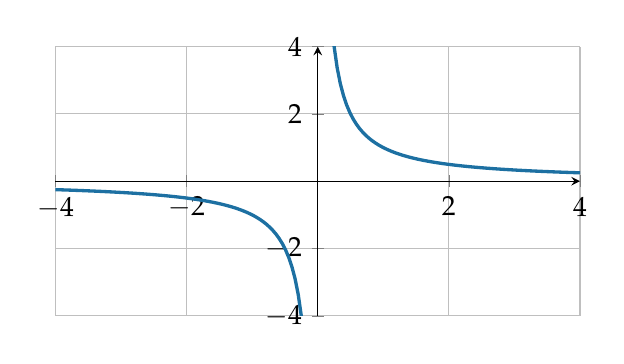
\begin{tikzpicture}\begin{axis}[width=.68\textwidth,height=5cm,axis lines=middle,xmin=-4,xmax=4,ymin=-4,ymax=4,grid=major]\addplot[Blue,very thick,samples=80,domain=-4:-.15]{1/x};\addplot[Blue,very thick,samples=80,domain=.15:4]{1/x};\end{axis}\end{tikzpicture}\end{center}
\end{activite}
\enseignant{$f'(x)=\dfrac{(x-4)(x+4)}{x^2}$ ; minimum $f(4)=8$. Faire verbaliser la donnée qui déclenche le choix de méthode.}

\begin{traceecrite}Pour une fonction contenant $\dfrac1x$, commencer par exclure $x=0$, puis dériver, factoriser et étudier le signe avant les variations.\end{traceecrite}

\begin{exemple}
Reprendre les données de l'activité et rédiger la solution dans l'ordre : définition des objets, propriété utilisée, calcul exact ou approché, puis phrase de réponse. La réponse modèle figure dans l'édition enseignant.
\end{exemple}
\enseignant{$f'(x)=\dfrac{(x-4)(x+4)}{x^2}$ ; minimum $f(4)=8$.}

\begin{exercice}[-- essentiel]
\begin{enumerate}\item Choisir entre suite arithmétique, suite géométrique et fonction exponentielle dans trois situations.\item Résoudre une équation exponentielle avec un logarithme.\item Calculer une probabilité à partir d'un arbre puis interpréter.\end{enumerate}
\end{exercice}
\enseignant{Justifier chaque choix par variation absolue ou relative ; vérifier la positivité avant le logarithme ; multiplier le long d'un chemin et conclure par une phrase.}

\manuelref{Calao, p. 94, n° 1 à 9, puis p. 96, n° 10 à 21}
\ExoSession{55}

\begin{dm}Reprendre l'exercice d'entraînement 2 avec les données suivantes : remplacer la donnée initiale par $395$ et le taux ou la raison par $3$. Rédiger en quatre lignes : données, formule, calcul, conclusion.\end{dm}
\enseignant{La correction dépend de l'exercice repris. Vérifier surtout la cohérence du modèle, le nombre d'itérations, l'arrondi et la phrase de conclusion.}

\begin{sortie}Sur une demi-feuille : écrire la règle principale de la séance, traiter un exemple très court et indiquer son degré de confiance de 1 à 4. Question(s) essentielle(s) du jour : 1, 2 et 3.\end{sortie}

\ifprof
\begin{methode}
\textbf{Conduite en 1 h :} 7 min d'automatismes ; 10 min de mise en commun et trace ; 28 min d'exercices essentiels ; 5 min de correction ; 3 min de billet de sortie.\\
\textbf{Conduite en 2 h :} ajouter 20 min de recherche de l'activité, 20 min d'institutionnalisation, un second exercice autonome et 10 min de correction comparée.\\
\textbf{Différenciation :} fournir aux élèves fragiles une fiche à quatre cases (données, modèle, calcul, conclusion). Demander aux élèves rapides de produire un contre-exemple, une justification ou une seconde méthode.
\end{methode}
\fi

\appendix
\chapter{Devoirs surveillés}
Deux versions sont proposées pour chaque chapitre. La structure de référence est : automatismes sur 6 points, exercice sur 6 points et problème sur 8 points.
\section*{Chapitre 1 -- Suites numériques}
\dsheader{1}{A}{Suites numériques}{modéliser, calculer, raisonner, communiquer}
\begin{exercice}[1 -- Automatismes]\points{6}
\begin{enumerate}
\item Donner le coefficient multiplicateur associé à une hausse de $5\,\%$.
\item La suite $12,17,22,27,\ldots$ est-elle arithmétique ? Donner sa raison.
\item Combien de termes contient $u_4+u_5+\cdots+u_{18}$ ?
\item Si $w_0=80$ et $w_{n+1}=0{,}9w_n$, calculer $w_2$.
\item Écrire $1+2+\cdots+20$ à l'aide du symbole $\sum$.
\end{enumerate}
\end{exercice}
\begin{exercice}[2 -- Abonnements]\points{6}
Une plateforme compte $120\,000$ abonnés au début de l'année et en gagne $11\,000$ chaque mois. On note $u_n$ le nombre d'abonnés, en milliers, après $n$ mois.
\begin{enumerate}
\item Justifier que $(u_n)$ est arithmétique et préciser sa raison.
\item Exprimer $u_n$ en fonction de $n$, puis calculer $u_{12}$.
\item Calculer $u_1+\cdots+u_{12}$. Interpréter cette somme avec prudence.
\end{enumerate}
\end{exercice}
\begin{exercice}[3 -- Placement et objectif]\points{8}
Un capital initial de $650\,000$ Ar augmente de $5\,\%$ par an. On note $C_n$ le capital après $n$ années.
\begin{enumerate}
\item Écrire $C_{n+1}$ en fonction de $C_n$, puis $C_n$ en fonction de $n$.
\item Calculer $C_5$, arrondi à l'ariary.
\item Déterminer à la calculatrice le premier entier $n$ pour lequel $C_n$ dépasse $1\,000\,000$ Ar.
\item Expliquer pourquoi le modèle est géométrique et non arithmétique.
\end{enumerate}
\end{exercice}
\enseignant{\textbf{Barème.} Ex. 1 : 6 points répartis sur les automatismes. Ex. 2 : 6 points. Ex. 3 : 8 points.\\
\textbf{Éléments de correction.} Le coefficient est $1{,}05$. La première suite flash est arithmétique de raison $5$ ; la somme contient $15$ termes ; $w_2=64$ et $\sum_{k=1}^{20}k$. Pour l'exercice 2, $u_n=120+11n$, donc $u_{12}=252$ ; la somme demandée utilise $12\dfrac{u_1+u_{12}}2$ et cumule des états mensuels, pas un nombre de personnes distinctes. Pour l'exercice 3, $C_n=650\,000\times\left(1+\dfrac{5}{100}\right)^n$ ; contrôler le seuil par deux valeurs consécutives.}

\dsheader{1}{B}{Suites numériques}{modéliser, calculer, raisonner, communiquer}
\begin{exercice}[1 -- Automatismes]\points{6}
\begin{enumerate}
\item Donner le coefficient multiplicateur associé à une hausse de $4\,\%$.
\item La suite $12,17,22,27,\ldots$ est-elle arithmétique ? Donner sa raison.
\item Combien de termes contient $u_4+u_5+\cdots+u_{18}$ ?
\item Si $w_0=80$ et $w_{n+1}=0{,}9w_n$, calculer $w_2$.
\item Écrire $1+2+\cdots+20$ à l'aide du symbole $\sum$.
\end{enumerate}
\end{exercice}
\begin{exercice}[2 -- Abonnements]\points{6}
Une plateforme compte $145\,000$ abonnés au début de l'année et en gagne $9\,000$ chaque mois. On note $u_n$ le nombre d'abonnés, en milliers, après $n$ mois.
\begin{enumerate}
\item Justifier que $(u_n)$ est arithmétique et préciser sa raison.
\item Exprimer $u_n$ en fonction de $n$, puis calculer $u_{12}$.
\item Calculer $u_1+\cdots+u_{12}$. Interpréter cette somme avec prudence.
\end{enumerate}
\end{exercice}
\begin{exercice}[3 -- Placement et objectif]\points{8}
Un capital initial de $720\,000$ Ar augmente de $4\,\%$ par an. On note $C_n$ le capital après $n$ années.
\begin{enumerate}
\item Écrire $C_{n+1}$ en fonction de $C_n$, puis $C_n$ en fonction de $n$.
\item Calculer $C_5$, arrondi à l'ariary.
\item Déterminer à la calculatrice le premier entier $n$ pour lequel $C_n$ dépasse $1\,000\,000$ Ar.
\item Expliquer pourquoi le modèle est géométrique et non arithmétique.
\end{enumerate}
\end{exercice}
\enseignant{\textbf{Barème.} Ex. 1 : 6 points répartis sur les automatismes. Ex. 2 : 6 points. Ex. 3 : 8 points.\\
\textbf{Éléments de correction.} Le coefficient est $1{,}04$. La première suite flash est arithmétique de raison $5$ ; la somme contient $15$ termes ; $w_2=64$ et $\sum_{k=1}^{20}k$. Pour l'exercice 2, $u_n=145+9n$, donc $u_{12}=253$ ; la somme demandée utilise $12\dfrac{u_1+u_{12}}2$ et cumule des états mensuels, pas un nombre de personnes distinctes. Pour l'exercice 3, $C_n=720\,000\times\left(1+\dfrac{4}{100}\right)^n$ ; contrôler le seuil par deux valeurs consécutives.}

\section*{Chapitre 2 -- Fonctions exponentielles}
\dsheader{2}{A}{Fonctions exponentielles}{calculer, représenter, modéliser, interpréter}
\begin{exercice}[1 -- Puissances et variations]\points{6}
\begin{enumerate}
\item Simplifier $2^4\times2^{-7}$ et $\dfrac{5^{x+3}}{5^x}$.
\item Écrire $3^{-2}$ sous forme de fraction.
\item Donner le sens de variation de $f(x)=1{,}04^x$ et de $g(x)=-2\times0{,}75^x$.
\item Expliquer pourquoi $a^x+a^y=a^{x+y}$ est fausse en général.
\end{enumerate}
\end{exercice}
\begin{exercice}[2 -- Fréquentation d'un site]\points{6}
Au lancement, un site reçoit $2400$ visites par jour. La fréquentation augmente de $4\,\%$ par semaine. On modélise par $V(t)=2400\times1{,}04^t$.
\begin{enumerate}
\item Interpréter les nombres $2400$ et $1{,}04$.
\item Calculer $V(8)$, arrondi à l'unité.
\item Déterminer le premier nombre entier de semaines pour lequel $V(t)>3100$.
\end{enumerate}
\end{exercice}
\begin{exercice}[3 -- Taux moyen]\points{8}
Le chiffre d'affaires d'une entreprise passe de $82\,000$ à $104000$ euros en quatre ans.
\begin{enumerate}
\item Calculer le coefficient global.
\item Écrire le coefficient annuel moyen sous la forme d'une puissance.
\item Calculer le taux annuel moyen, arrondi à $0{,}01\,\%$.
\item Expliquer pourquoi on ne divise pas simplement le taux global par quatre.
\end{enumerate}
\end{exercice}
\enseignant{\textbf{Barème :} $6+6+8$. \textbf{Correction :} $2^4\times2^{-7}=2^{-3}=\dfrac18$, $\dfrac{5^{x+3}}{5^x}=125$, $3^{-2}=\dfrac19$. $f$ est croissante et $g$ croissante. Dans le problème, calculer $V(8)$ puis tester deux entiers consécutifs autour du seuil. Pour le taux moyen, $q=\left(\dfrac{V_f}{V_i}\right)^{\frac14}$ et $t=q-1$ ; les coefficients se multiplient.}

\dsheader{2}{B}{Fonctions exponentielles}{calculer, représenter, modéliser, interpréter}
\begin{exercice}[1 -- Puissances et variations]\points{6}
\begin{enumerate}
\item Simplifier $2^4\times2^{-7}$ et $\dfrac{5^{x+3}}{5^x}$.
\item Écrire $3^{-2}$ sous forme de fraction.
\item Donner le sens de variation de $f(x)=1{,}03^x$ et de $g(x)=-2\times0{,}75^x$.
\item Expliquer pourquoi $a^x+a^y=a^{x+y}$ est fausse en général.
\end{enumerate}
\end{exercice}
\begin{exercice}[2 -- Fréquentation d'un site]\points{6}
Au lancement, un site reçoit $1850$ visites par jour. La fréquentation augmente de $3\,\%$ par semaine. On modélise par $V(t)=1850\times1{,}03^t$.
\begin{enumerate}
\item Interpréter les nombres $1850$ et $1{,}03$.
\item Calculer $V(8)$, arrondi à l'unité.
\item Déterminer le premier nombre entier de semaines pour lequel $V(t)>2250$.
\end{enumerate}
\end{exercice}
\begin{exercice}[3 -- Taux moyen]\points{8}
Le chiffre d'affaires d'une entreprise passe de $82\,000$ à $98000$ euros en quatre ans.
\begin{enumerate}
\item Calculer le coefficient global.
\item Écrire le coefficient annuel moyen sous la forme d'une puissance.
\item Calculer le taux annuel moyen, arrondi à $0{,}01\,\%$.
\item Expliquer pourquoi on ne divise pas simplement le taux global par quatre.
\end{enumerate}
\end{exercice}
\enseignant{\textbf{Barème :} $6+6+8$. \textbf{Correction :} $2^4\times2^{-7}=2^{-3}=\dfrac18$, $\dfrac{5^{x+3}}{5^x}=125$, $3^{-2}=\dfrac19$. $f$ est croissante et $g$ croissante. Dans le problème, calculer $V(8)$ puis tester deux entiers consécutifs autour du seuil. Pour le taux moyen, $q=\left(\dfrac{V_f}{V_i}\right)^{\frac14}$ et $t=q-1$ ; les coefficients se multiplient.}

\section*{Chapitre 3 -- Fonction logarithme décimal}
\dsheader{3}{A}{Logarithme décimal}{calculer, résoudre, raisonner, communiquer}
\begin{exercice}[1 -- Connaissances et calculs]\points{6}
\begin{enumerate}
\item Calculer $\log(1000)$, $\log(0{,}01)$ et $\log(10^{-4})$.
\item Pour $x,y>0$, développer $\log\!\left(\dfrac{100x^3}{y} \right)$.
\item Résoudre $10^t=28000$ et donner $t$ au centième.
\end{enumerate}
\end{exercice}
\begin{exercice}[2 -- Objectif de croissance]\points{6}
Une valeur est multipliée chaque année par $1{,}05$. On cherche le temps nécessaire pour qu'elle double.
\begin{enumerate}
\item Traduire le problème par une équation.
\item Résoudre cette équation à l'aide du logarithme décimal.
\item Donner le premier nombre entier d'années permettant d'atteindre ou dépasser le double.
\item Vérifier avec les deux puissances consécutives utiles.
\end{enumerate}
\end{exercice}
\begin{exercice}[3 -- Niveau sonore]\points{8}
Le niveau sonore est $L=10\log\!\left(\dfrac I{I_0}\right)$, en décibels.
\begin{enumerate}
\item Calculer $L$ lorsque $I=10^6I_0$.
\item Pour $L=84$, exprimer puis calculer le rapport $\dfrac I{I_0}$.
\item Comparer les intensités correspondant à $84$ dB et à $74$ dB.
\end{enumerate}
\end{exercice}
\enseignant{\textbf{Barème :} $6+6+8$. \textbf{Correction :} Les valeurs usuelles sont $3,-2,-4$. Le développement donne $2+3\log x-\log y$. $t=\log(28000)$. Pour le doublement, $x=\dfrac{\log2}{\log(1{,}05)}$ puis on prend l'entier supérieur et on contrôle. $\dfrac I{I_0}=10^{\frac L{10}}$ ; un écart de $10$ dB correspond à une intensité multipliée par $10$.}

\dsheader{3}{B}{Logarithme décimal}{calculer, résoudre, raisonner, communiquer}
\begin{exercice}[1 -- Connaissances et calculs]\points{6}
\begin{enumerate}
\item Calculer $\log(1000)$, $\log(0{,}01)$ et $\log(10^{-4})$.
\item Pour $x,y>0$, développer $\log\!\left(\dfrac{100x^3}{y} \right)$.
\item Résoudre $10^t=32000$ et donner $t$ au centième.
\end{enumerate}
\end{exercice}
\begin{exercice}[2 -- Objectif de croissance]\points{6}
Une valeur est multipliée chaque année par $1{,}07$. On cherche le temps nécessaire pour qu'elle double.
\begin{enumerate}
\item Traduire le problème par une équation.
\item Résoudre cette équation à l'aide du logarithme décimal.
\item Donner le premier nombre entier d'années permettant d'atteindre ou dépasser le double.
\item Vérifier avec les deux puissances consécutives utiles.
\end{enumerate}
\end{exercice}
\begin{exercice}[3 -- Niveau sonore]\points{8}
Le niveau sonore est $L=10\log\!\left(\dfrac I{I_0}\right)$, en décibels.
\begin{enumerate}
\item Calculer $L$ lorsque $I=10^6I_0$.
\item Pour $L=78$, exprimer puis calculer le rapport $\dfrac I{I_0}$.
\item Comparer les intensités correspondant à $78$ dB et à $68$ dB.
\end{enumerate}
\end{exercice}
\enseignant{\textbf{Barème :} $6+6+8$. \textbf{Correction :} Les valeurs usuelles sont $3,-2,-4$. Le développement donne $2+3\log x-\log y$. $t=\log(32000)$. Pour le doublement, $x=\dfrac{\log2}{\log(1{,}07)}$ puis on prend l'entier supérieur et on contrôle. $\dfrac I{I_0}=10^{\frac L{10}}$ ; un écart de $10$ dB correspond à une intensité multipliée par $10$.}

\section*{Chapitre 4 -- Fonction inverse}
\dsheader{4}{A}{Fonction inverse}{calculer, raisonner, représenter, communiquer}
\begin{exercice}[1 -- Fonction inverse]\points{6}
On considère $f(x)=2+\dfrac{16}x$.
\begin{enumerate}
\item Donner son domaine.
\item Calculer sa dérivée et étudier son signe.
\item Donner ses asymptotes et son sens de variation sur chaque intervalle du domaine.
\end{enumerate}
\end{exercice}
\begin{exercice}[2 -- Tableau de signes]\points{6}
Résoudre $\dfrac{(x-4)(x+2)}x\geq0$. Le tableau doit faire apparaître les zéros et la valeur interdite.
\end{exercice}
\begin{exercice}[3 -- Coût moyen]\points{8}
Pour $x>0$, un coût moyen est modélisé par $C(x)=x+\dfrac{16}x+12$.
\begin{enumerate}
\item Calculer $C'(x)$ et factoriser son numérateur.
\item Dresser le tableau de variations de $C$ sur $]0,+\infty[$.
\item Déterminer la valeur de $x$ qui minimise le coût moyen et calculer ce minimum.
\item Faire une esquisse cohérente de la courbe.
\end{enumerate}
\end{exercice}
\enseignant{\textbf{Barème :} $6+6+8$. \textbf{Correction :} $D_f=\R\setminus\{0\}$, $f'(x)=-\dfrac{16}{x^2}<0$, asymptotes $x=0$ et $y=2$. Pour le quotient, ordonner $-2,0,4$ et exclure $0$. Pour le coût, $C'(x)=1-\dfrac{16}{x^2}=\dfrac{(x-4)(x+4)}{x^2}$ ; minimum en $x=4$, de valeur $20$.}

\dsheader{4}{B}{Fonction inverse}{calculer, raisonner, représenter, communiquer}
\begin{exercice}[1 -- Fonction inverse]\points{6}
On considère $f(x)=2+\dfrac{9}x$.
\begin{enumerate}
\item Donner son domaine.
\item Calculer sa dérivée et étudier son signe.
\item Donner ses asymptotes et son sens de variation sur chaque intervalle du domaine.
\end{enumerate}
\end{exercice}
\begin{exercice}[2 -- Tableau de signes]\points{6}
Résoudre $\dfrac{(x-3)(x+2)}x\geq0$. Le tableau doit faire apparaître les zéros et la valeur interdite.
\end{exercice}
\begin{exercice}[3 -- Coût moyen]\points{8}
Pour $x>0$, un coût moyen est modélisé par $C(x)=x+\dfrac{9}x+12$.
\begin{enumerate}
\item Calculer $C'(x)$ et factoriser son numérateur.
\item Dresser le tableau de variations de $C$ sur $]0,+\infty[$.
\item Déterminer la valeur de $x$ qui minimise le coût moyen et calculer ce minimum.
\item Faire une esquisse cohérente de la courbe.
\end{enumerate}
\end{exercice}
\enseignant{\textbf{Barème :} $6+6+8$. \textbf{Correction :} $D_f=\R\setminus\{0\}$, $f'(x)=-\dfrac{9}{x^2}<0$, asymptotes $x=0$ et $y=2$. Pour le quotient, ordonner $-2,0,3$ et exclure $0$. Pour le coût, $C'(x)=1-\dfrac{9}{x^2}=\dfrac{(x-3)(x+3)}{x^2}$ ; minimum en $x=3$, de valeur $18$.}

\section*{Chapitre 5 -- Statistiques à deux variables quantitatives}
\dsheader{5}{A}{Statistiques à deux variables}{représenter, modéliser, calculer, interpréter}
\begin{exercice}[1 -- Construire et décrire]\points{6}
On observe les couples $(1;8)$, $(2;11)$, $(3;13)$, $(4;17)$, $(5;19)$ et $(6;23)$.
\begin{enumerate}
\item Représenter le nuage dans un repère correctement légendé.
\item Calculer les coordonnées du point moyen.
\item Décrire la tendance et la dispersion sans conclure à une causalité.
\end{enumerate}
\end{exercice}
\begin{exercice}[2 -- Exploiter un ajustement]\points{6}
Une droite d'ajustement est $y=3{,}2x+12$, établie pour $x\in[2,15]$.
\begin{enumerate}
\item Estimer $y$ pour $x=10$ et qualifier l'estimation.
\item Estimer $x$ lorsque $y=60$.
\item Estimer $y$ pour $x=40$, puis expliquer pourquoi ce résultat doit être considéré avec prudence.
\end{enumerate}
\end{exercice}
\begin{exercice}[3 -- Changement de variable]\points{8}
On pose $z=\log(y)$ et l'ajustement de $(x,z)$ est $z=0{,}06x+1{,}1$.
\begin{enumerate}
\item Exprimer $y$ en fonction de $x$.
\item Estimer $y$ pour $x=8$.
\item Expliquer l'intérêt du changement de variable et une limite de l'extrapolation.
\end{enumerate}
\end{exercice}
\enseignant{\textbf{Barème :} $6+6+8$. \textbf{Correction :} Calculer $\bar x$ et $\bar y$ à partir des six valeurs. Avec la droite, substituer $x$ ou résoudre une équation ; $x=10$ est une interpolation et $x=40$ une extrapolation éloignée. Le dernier modèle est $y=10^{0{,}06x+1{,}1}$.}

\dsheader{5}{B}{Statistiques à deux variables}{représenter, modéliser, calculer, interpréter}
\begin{exercice}[1 -- Construire et décrire]\points{6}
On observe les couples $(1;8)$, $(2;11)$, $(3;13)$, $(4;17)$, $(5;22)$ et $(6;23)$.
\begin{enumerate}
\item Représenter le nuage dans un repère correctement légendé.
\item Calculer les coordonnées du point moyen.
\item Décrire la tendance et la dispersion sans conclure à une causalité.
\end{enumerate}
\end{exercice}
\begin{exercice}[2 -- Exploiter un ajustement]\points{6}
Une droite d'ajustement est $y=2{,}4x+18$, établie pour $x\in[2,15]$.
\begin{enumerate}
\item Estimer $y$ pour $x=10$ et qualifier l'estimation.
\item Estimer $x$ lorsque $y=60$.
\item Estimer $y$ pour $x=40$, puis expliquer pourquoi ce résultat doit être considéré avec prudence.
\end{enumerate}
\end{exercice}
\begin{exercice}[3 -- Changement de variable]\points{8}
On pose $z=\log(y)$ et l'ajustement de $(x,z)$ est $z=0{,}06x+1{,}1$.
\begin{enumerate}
\item Exprimer $y$ en fonction de $x$.
\item Estimer $y$ pour $x=8$.
\item Expliquer l'intérêt du changement de variable et une limite de l'extrapolation.
\end{enumerate}
\end{exercice}
\enseignant{\textbf{Barème :} $6+6+8$. \textbf{Correction :} Calculer $\bar x$ et $\bar y$ à partir des six valeurs. Avec la droite, substituer $x$ ou résoudre une équation ; $x=10$ est une interpolation et $x=40$ une extrapolation éloignée. Le dernier modèle est $y=10^{0{,}06x+1{,}1}$.}

\section*{Chapitre 6 -- Probabilités conditionnelles}
\dsheader{6}{A}{Probabilités conditionnelles}{modéliser, calculer, raisonner, interpréter}
\begin{exercice}[1 -- Arbre pondéré]\points{6}
Une proportion 0{,}35 des commandes est express. Le taux de retard est 0{,}05 parmi les commandes express et 0{,}12 parmi les autres.
\begin{enumerate}
\item Définir les événements $E$ et $R$, puis construire l'arbre pondéré complet.
\item Calculer $P(E\cap R)$.
\item Calculer $P(R)$ par la formule des probabilités totales.
\item Calculer $P_R(E)$ et interpréter.
\end{enumerate}
\end{exercice}
\begin{exercice}[2 -- Indépendance]\points{6}
Dans une autre étude, $P(A)=0{,}4$, $P(B)=0{,}25$ et $P(A\cap B)=0{,}10$.
\begin{enumerate}
\item Calculer $P(A)P(B)$.
\item Les événements sont-ils indépendants ? Justifier.
\item Calculer $P_A(B)$ et confirmer la conclusion.
\end{enumerate}
\end{exercice}
\begin{exercice}[3 -- Tableau d'effectifs]\points{8}
Sur $800$ clients, $320$ ont une carte premium ; $96$ clients premium et $72$ clients non premium ont résilié. Construire le tableau complet puis calculer la probabilité d'être premium sachant que le client a résilié.
\end{exercice}
\enseignant{\textbf{Barème :} $8+6+6$. \textbf{Correction :} $P(R)=P(E)P_E(R)+P(\overline E)P_{\overline E}(R)$ puis $P_R(E)=\dfrac{P(E\cap R)}{P(R)}$. Pour l'indépendance, comparer l'intersection au produit $0{,}10$. Dans le tableau, il y a $168$ résiliations, donc $P_R(P)=\dfrac{96}{168}=\dfrac47$.}

\dsheader{6}{B}{Probabilités conditionnelles}{modéliser, calculer, raisonner, interpréter}
\begin{exercice}[1 -- Arbre pondéré]\points{6}
Une proportion 0{,}45 des commandes est express. Le taux de retard est 0{,}08 parmi les commandes express et 0{,}15 parmi les autres.
\begin{enumerate}
\item Définir les événements $E$ et $R$, puis construire l'arbre pondéré complet.
\item Calculer $P(E\cap R)$.
\item Calculer $P(R)$ par la formule des probabilités totales.
\item Calculer $P_R(E)$ et interpréter.
\end{enumerate}
\end{exercice}
\begin{exercice}[2 -- Indépendance]\points{6}
Dans une autre étude, $P(A)=0{,}4$, $P(B)=0{,}25$ et $P(A\cap B)=0{,}14$.
\begin{enumerate}
\item Calculer $P(A)P(B)$.
\item Les événements sont-ils indépendants ? Justifier.
\item Calculer $P_A(B)$ et confirmer la conclusion.
\end{enumerate}
\end{exercice}
\begin{exercice}[3 -- Tableau d'effectifs]\points{8}
Sur $800$ clients, $320$ ont une carte premium ; $96$ clients premium et $72$ clients non premium ont résilié. Construire le tableau complet puis calculer la probabilité d'être premium sachant que le client a résilié.
\end{exercice}
\enseignant{\textbf{Barème :} $8+6+6$. \textbf{Correction :} $P(R)=P(E)P_E(R)+P(\overline E)P_{\overline E}(R)$ puis $P_R(E)=\dfrac{P(E\cap R)}{P(R)}$. Pour l'indépendance, comparer l'intersection au produit $0{,}10$. Dans le tableau, il y a $168$ résiliations, donc $P_R(P)=\dfrac{96}{168}=\dfrac47$.}

\section*{Chapitre 7 -- Variables aléatoires discrètes et loi binomiale}
\dsheader{7}{A}{Variables aléatoires et loi binomiale}{modéliser, calculer, raisonner, interpréter}
\begin{exercice}[1 -- Espérance d'un jeu]\points{6}
Un jeu coûte $3$ euros. Le gain brut vaut $0$, $5$ ou $15$ euros avec probabilités $0{,}65$, $0{,}25$ et $0{,}10$.
\begin{enumerate}
\item Construire la loi du gain net $G$.
\item Calculer $E(G)$.
\item Le jeu est-il favorable au joueur ? Interpréter sans affirmer ce qui arrivera lors d'une partie.
\end{enumerate}
\end{exercice}
\begin{exercice}[2 -- Loi binomiale]\points{6}
Un client répond favorablement avec probabilité $0{,}30$. Un conseiller contacte indépendamment $10$ clients. On note $X$ le nombre de réponses favorables.
\begin{enumerate}
\item Justifier la loi de $X$ et donner ses paramètres.
\item Calculer $P(X=2)$.
\item Calculer $P(X=0)$ puis $P(X\geq1)$.
\item Calculer et interpréter $E(X)$.
\end{enumerate}
\end{exercice}
\begin{exercice}[3 -- Triangle de Pascal]\points{8}
\begin{enumerate}
\item Écrire la ligne $n=6$ du triangle de Pascal.
\item Lire $\binom62$ et $\binom64$.
\item Expliquer le rôle de $\binom nk$ dans la formule binomiale.
\end{enumerate}
\end{exercice}
\enseignant{\textbf{Barème :} $6+8+6$. \textbf{Correction :} Le gain net vaut $-3,2,12$ ; $E(G)=-1{,}95+0{,}50+1{,}20=-0{,}25$ euro. $X\sim\mathcal B(10,0{,}30)$ ; appliquer la formule, utiliser $1-P(X=0)$ pour « au moins un », et $E(X)=np$. La ligne $n=6$ est $1,6,15,20,15,6,1$.}

\dsheader{7}{B}{Variables aléatoires et loi binomiale}{modéliser, calculer, raisonner, interpréter}
\begin{exercice}[1 -- Espérance d'un jeu]\points{6}
Un jeu coûte $3$ euros. Le gain brut vaut $0$, $5$ ou $15$ euros avec probabilités $0{,}65$, $0{,}25$ et $0{,}10$.
\begin{enumerate}
\item Construire la loi du gain net $G$.
\item Calculer $E(G)$.
\item Le jeu est-il favorable au joueur ? Interpréter sans affirmer ce qui arrivera lors d'une partie.
\end{enumerate}
\end{exercice}
\begin{exercice}[2 -- Loi binomiale]\points{6}
Un client répond favorablement avec probabilité $0{,}25$. Un conseiller contacte indépendamment $8$ clients. On note $X$ le nombre de réponses favorables.
\begin{enumerate}
\item Justifier la loi de $X$ et donner ses paramètres.
\item Calculer $P(X=2)$.
\item Calculer $P(X=0)$ puis $P(X\geq1)$.
\item Calculer et interpréter $E(X)$.
\end{enumerate}
\end{exercice}
\begin{exercice}[3 -- Triangle de Pascal]\points{8}
\begin{enumerate}
\item Écrire la ligne $n=6$ du triangle de Pascal.
\item Lire $\binom62$ et $\binom64$.
\item Expliquer le rôle de $\binom nk$ dans la formule binomiale.
\end{enumerate}
\end{exercice}
\enseignant{\textbf{Barème :} $6+8+6$. \textbf{Correction :} Le gain net vaut $-3,2,12$ ; $E(G)=-1{,}95+0{,}50+1{,}20=-0{,}25$ euro. $X\sim\mathcal B(8,0{,}25)$ ; appliquer la formule, utiliser $1-P(X=0)$ pour « au moins un », et $E(X)=np$. La ligne $n=6$ est $1,6,15,20,15,6,1$.}

\chapter{Formulaire raisonné}
\begin{longtable}{p{.23\textwidth}p{.33\textwidth}p{.35\textwidth}}
\toprule
Objet & Formule & Contrôle à effectuer\\
\midrule
Suite arithmétique & $u_n=u_0+nr$ & Le rang initial est-il $0$ ou $1$ ?\\
Somme arithmétique & $N\dfrac{\text{premier}+\text{dernier}}2$ & Compter les termes : dernier rang $-$ premier rang $+1$.\\
Suite géométrique & $u_n=u_0q^n$ & $q$ est-il un coefficient et non un pourcentage ?\\
Somme géométrique & $u_0\dfrac{1-q^{n+1}}{1-q}$ & $q\neq1$ et $n+1$ termes.\\
Taux moyen & $q=Q^{\frac1n}$, $t=q-1$ & Ne pas diviser le taux global par $n$.\\
Logarithme & $a^x=b\iff x=\dfrac{\log b}{\log a}$ & $a>0$, $a\neq1$, $b>0$.\\
Fonction inverse & $\left(\dfrac1x\right)'=-\dfrac1{x^2}$ & Exclure $x=0$.\\
Ajustement affine & $y=ax+b$ & Estimation, domaine observé, unité.\\
Conditionnement & $P_A(B)=\dfrac{P(A\cap B)}{P(A)}$ & $P(A)>0$ et ordre du conditionnement.\\
Probabilités totales & $P(B)=\sum_iP(A_i)P_{A_i}(B)$ & Les $A_i$ forment-ils une partition ?\\
Loi binomiale & $P(X=k)=\binom nkp^k(1-p)^{n-k}$ & Indépendance, même $p$, $0\leq k\leq n$.\\
Espérance binomiale & $E(X)=np$ & Interprétation moyenne à long terme.\\
\bottomrule
\end{longtable}

\chapter{Tableau de pilotage des 55 séances}
\small
\begin{longtable}{cclp{.42\textwidth}}
\toprule
N° & Date & Chapitre & Objet\\
\midrule\endhead
1 & 15/09/2026 & Suites numériques & Suite arithmétique : reconnaître et modéliser\\
2 & 17/09/2026 & Suites numériques & Suite arithmétique : terme général\\
3 & 22/09/2026 & Suites numériques & Somme des termes d'une suite arithmétique\\
4 & 24/09/2026 & Suites numériques & Suite géométrique : reconnaître et modéliser\\
5 & 29/09/2026 & Suites numériques & Suite géométrique : terme général et somme\\
6 & 01/10/2026 & Suites numériques & Bilan et évaluation formative\\
7 & 06/10/2026 & Fonctions exponentielles & Définition et sens de variation de $a^x$\\
8 & 08/10/2026 & Fonctions exponentielles & Puissances et propriétés algébriques\\
9 & 13/10/2026 & Fonctions exponentielles & Fonctions $x\mapsto k a^x$ : variations et graphique\\
10 & 15/10/2026 & Fonctions exponentielles & Taux d'évolution moyen\\
11 & 03/11/2026 & Fonctions exponentielles & Lecture de représentations graphiques\\
12 & 05/11/2026 & Fonctions exponentielles & Équations exponentielles simples\\
13 & 10/11/2026 & Fonctions exponentielles & Modélisation par une fonction exponentielle\\
14 & 12/11/2026 & Fonctions exponentielles & Bilan et évaluation du chapitre\\
15 & 17/11/2026 & Fonction logarithme décimal & Définition du logarithme décimal\\
16 & 19/11/2026 & Fonction logarithme décimal & Sens de variation et représentation\\
17 & 24/11/2026 & Fonction logarithme décimal & Propriétés algébriques\\
18 & 26/11/2026 & Fonction logarithme décimal & Résoudre $10^x=b$\\
19 & 01/12/2026 & Fonction logarithme décimal & Résoudre $a^x=b$\\
20 & 03/12/2026 & Fonction logarithme décimal & Équations $x^a=b$ et inégalités simples\\
21 & 08/12/2026 & Fonction logarithme décimal & Problèmes contextualisés\\
22 & 10/12/2026 & Fonction logarithme décimal & Bilan et évaluation\\
23 & 15/12/2026 & Fonction inverse & Définition et courbe de la fonction inverse\\
24 & 17/12/2026 & Fonction inverse & Comportement aux bornes et asymptotes\\
25 & 05/01/2027 & Fonction inverse & Dérivée et sens de variation\\
26 & 07/01/2027 & Fonction inverse & Combinaisons avec des fonctions polynomiales\\
27 & 12/01/2027 & Fonction inverse & Signe et factorisation\\
28 & 14/01/2027 & Fonction inverse & Dérivées de polynômes de degré au plus 3\\
29 & 19/01/2027 & Fonction inverse & Étude complète et représentation\\
30 & 21/01/2027 & Fonction inverse & Bilan et évaluation\\
31 & 26/01/2027 & Statistiques à deux variables & Nuage de points\\
32 & 28/01/2027 & Statistiques à deux variables & Lecture et interprétation du nuage\\
33 & 02/02/2027 & Statistiques à deux variables & Ajustement affine\\
34 & 04/02/2027 & Statistiques à deux variables & Interpolation\\
35 & 09/02/2027 & Statistiques à deux variables & Extrapolation\\
36 & 11/02/2027 & Statistiques à deux variables & Changement de variable\\
37 & 02/03/2027 & Statistiques à deux variables & Choix du modèle et ajustement\\
38 & 04/03/2027 & Statistiques à deux variables & Bilan et évaluation\\
39 & 09/03/2027 & Probabilités conditionnelles & Conditionnement\\
40 & 11/03/2027 & Probabilités conditionnelles & Arbres pondérés\\
41 & 16/03/2027 & Probabilités conditionnelles & Produit des probabilités le long d'un chemin\\
42 & 18/03/2027 & Probabilités conditionnelles & Indépendance\\
43 & 23/03/2027 & Probabilités conditionnelles & Partition et probabilités totales\\
44 & 25/03/2027 & Probabilités conditionnelles & Problèmes contextualisés\\
45 & 30/03/2027 & Probabilités conditionnelles & Entraînement mixte\\
46 & 01/04/2027 & Probabilités conditionnelles & Bilan et évaluation\\
47 & 06/04/2027 & Variables aléatoires discrètes & Espérance d'une variable aléatoire\\
48 & 08/04/2027 & Variables aléatoires discrètes & Loi binomiale : reconnaître une situation\\
49 & 27/04/2027 & Variables aléatoires discrètes & Triangle de Pascal et coefficients binomiaux\\
50 & 29/04/2027 & Variables aléatoires discrètes & Probabilités binomiales\\
51 & 04/05/2027 & Variables aléatoires discrètes & Bilan du chapitre et évaluation\\
52 & 11/05/2027 & Révisions et consolidation & Diagnostic des acquis\\
53 & 13/05/2027 & Révisions et consolidation & Réactivation : fonctions exponentielles\\
54 & 18/05/2027 & Révisions et consolidation & Réactivation : logarithme décimal\\
55 & 20/05/2027 & Révisions et consolidation & Réactivation : fonction inverse\\
\bottomrule
\end{longtable}
\normalsize

\chapter{Sources et statut des contenus}
\begin{itemize}
\item Ministère de l'Éducation nationale, \emph{Programme de mathématiques de terminale technologique}, BO spécial n° 8 du 25 juillet 2019.
\item Éduscol, \emph{Programmes et ressources en mathématiques -- voie générale et technologique}, ressources institutionnelles consultées en septembre 2026.
\item \emph{Calao Mathématiques Terminale technologique}, manuel fourni par l'utilisateur, p. 18 à 169 pour les sept chapitres mobilisés. Chaque énoncé reproduit est accompagné de sa page et de son numéro ; l'édition professeur en propose une correction détaillée.
\item \emph{Progression Terminale STMG 2026--2027}, document fourni : calendrier, alternance des durées et ordre des notions.
\end{itemize}

\end{document}
